%
\documentclass[11pt, a4paper, twoside, openright]{report}

\usepackage{float} % lets you have non-floating floats
 
\usepackage{url} % for typesetting urls
 
%  We don't want figures to float so we define
% 
\newfloat{fig}{thp}{lof}[chapter]
\floatname{fig}{Figure}

%% These are standard LaTeX definitions for the document
%%
\title{Referential Integrity in\\ Cloud NoSQL Databases}
\author{Harsha Raja} 

%% This file can be used for creating a wide range of reports
%%  across various Schools
%%
%% Set up some things, mostly for the front page, for your specific document
%
% Current options are:
% [ecs|msor]              Which school you are in.
%
% [bschonscomp|]  Which degree you are doing
%                          You can also specify any other degree by name
%                          (see below)
% [font|image]            Use a font or an image for the VUW logo
%                          The font option will only work on ECS systems
%
\usepackage[image,ecs,meng]{vuwproject} 

% You should specifiy your supervisor here with
%     \supervisor{Firstname Lastname}
% use \supervisors if there are more than one supervisor
\supervisor{Dr. Pavle Mogin}
% Unless you've used the bschonscomp or mcompsci
%  options above use
% \otherdegree{MSc in Computer Science}
% here to specify degree

% Comment this out if you want the date printed.
%\date{}

\usepackage[bookmarks]{hyperref}
\usepackage{paralist}
\usepackage[utf8]{inputenc}
\usepackage[english]{babel}
\usepackage[numbers]{natbib}
\usepackage[enabled, chapter]{easy-todo}
\usepackage{blindtext}
\usepackage[boxed]{algorithm2e}
\usepackage{amsmath,amsfonts}
\usepackage{multirow}

\usepackage{subfigure}
\usepackage{ctable}
 \usepackage{setspace}
\usepackage{lscape}
\usepackage{colortbl}
\definecolor{light-gray}{gray}{0.85}
\newcommand{\rc}{\rowcolor{light-gray}}

\usepackage[printonlyused]{acronym}

%Article 1
\usepackage{units} %For Nice Fractions
\usepackage{caption2}
\newcommand{\nf}[2]{\nicefrac{#1}{#2}}
\usepackage{epsfig}

\newcommand{\Quote}[1]{``#1''}

%\renewcommand{\ac}[1]{#1}
%\renewcommand{\acf}[1]{#1}
%\renewcommand{\acp}[1]{#1s}

\hypersetup{
	pdftitle = {Cloud Computing},
	pdfauthor = {Harsha Raja},
	pdfkeywords = {}, 
	bookmarks=true
 	pdfborder={1 1 1},
	linkcolor = black,
	anchorcolor = black,
	citecolor = black,
	filecolor = black,
	urlcolor = black
}

\onehalfspacing
\begin{document}


% Make the page numbering roman, until after the contents, etc.
\frontmatter

%%%%%%%%%%%%%%%%%%%%%%%%%%%%%%%%%%%%%%%%%%%%%%%%%%%%%%%
 

\begin{abstract}
\small
% \blindtext
\end{abstract}

%%%%%%%%%%%%%%%%%%%%%%%%%%%%%%%%%%%%%%%%%%%%%%%%%%%%%%%
% \listoftodos
 \maketitle

\tableofcontents

%लाइन एक्सपान्देर
\acrodef{IT}{Information Technology}
\acrodef{API}{Application Programming Interface}

\acrodef{DBMS}{Database Management System}
\acrodef{RDBMS}{Relational Database Management System}
\acrodef{RDB}{Relational Database}
\acrodef{NoSQL}{Not only SQL}
\acrodef{blob}{Binary Large Objects}

\acrodef{ER}{Entity Relationship}
\acrodef{POJO}{Plain Old Java Object}
\acrodef{CRUD}{Create, Read, Update and Delete}

\acrodef{SaaS}{Software as a Service}
\acrodef{PaaS}{Platform as a Service}
\acrodef{IaaS}{Infrastructure as a Service}
\acrodef{DaaS}{Database as a Service}

\acrodef{1-NF}{First Normal Form}
\acrodef{3-NF}{Third Normal Form}
\acrodef{BCNF}{Boyce Codd Normal Form}

\acrodef{SEDA}{Staged Event-Driven Architecture}

\acrodef{PK}{Primary Key}
\acrodef{FK}{Foreign Key}

% \ac{IT} singular.
% \acp{IT} plural
% \acf{IT} Information Technology (IT)
 
\listoftodos

% we want a list of the figures we defined
%\listof{fig}{Figures}

%%%%%%%%%%%%%%%%%%%%%%%%%%%%%%%%%%%%%%%%%%%%%%%%%%%%%%%

\mainmatter

%%%%%%%%%%%%%%%%%%%%%%%%%%%%%%%%%%%%%%%%%%%%%%%%%%%%%%%
\acresetall
% 
% 
\chapter{Introduction} 
Cloud computing is a paradigm that is rapidly shifting the way IT services
and tools are being used. The fundamental reason is that it provides
 essential computing services that can be accessed through the Internet. 
 Amongst these services, cloud providers offer platforms that
 include hardware equipment and software applications, infrastructures such as
 servers and other network equipments, data storage and \acp{DBMS}, and
 others. All these services come with major benefits such as reduced maintenance
 costs,  automation of common tasks, and global access(\todo{cite (Wilkes,
 2010)} ). Moreover, such cloud
 services and other resources are hosted on the Internet and offered to  
 users for availing according to their needs.  Such characteristics made it
  natural for the  cloud to become  the backbone of application providers and
  users, and promoted the creation of novel theories and more applications to
 enhance the cloud .
 
  
  Cloud data storage is an important service that has been progressing, evolving
  and adapting alongside cloud computing. As the number of
  applications and users keep increasing, so does the demand for scalable, 
  efficient, and consistent data storage mechanisms offered by
  application providers. These storage mechanisms allow  users to store
  their data on the cloud without having to deal with the hassle of buying and
  maintaining database servers (\todo{cite SNIA}).

 The distributed nature of the cloud data storage, requires
 cloud \acp{DBMS} to satisfy essential requirements that are inherent to these
 environments. Some of these requirements are related to
  \begin{inparaenum}[a)]
 \item  scalability by matching the increase and decrease of active users
 and allowing the storage of large amounts of data,
 \item  robustness by maintaining several copies of data to make data
 available despite failures,
 \item  flexibility by allowing the storage of unstructured data, and
 \item  consistency of data by making sure data is never stale.
 \end{inparaenum}
   These requirements are not necessarily met by traditional \acp{RDBMS}. For
   example, scalability in \acp{RDBMS} is limited as these are designed to run
   on a single node. Robustness is lacking in terms of  a single point of
   failure would  make data unavailable. Also,     Thus, the  prevalent
   features of traditional \acp{RDBMS}  become issues when moved to the cloud.
    Nonetheless, there is still one characteristic that is desirable from
   \acp{RDBMS}: referential integrity in data.
   
   Referential integrity constraints  ensure that  relationships
   between data items are preserved. For example, it ensures that a course
   exists before students can enrol in it. Such relationships are 
   inherent to real-world data and have to be maintained in databases
   whether it is a traditional \ac{RDBMS} or a cloud \ac{DBMS}.
   Moreover, these constraints  ensure that no operations violate  the
   integrity between  data items (\todo{cite Navathe}).   Despite its
   importance, referential integrity is currently not a prominent feature in most  cloud
   column-oriented key-value \acp{DBMS}. 
   
   
   Column-oriented key-value \acp{DBMS}, also  referred simply to as cloud
   \ac{NoSQL} databases,  adopts the column-oriented key-value data model which
   is a widely used model for cloud \acp{DBMS}.These \acp{DBMS}  support many
   features required in cloud,  such as elastic scalability to match varying
   user demands, data replication,  schema-less data storage ,   and many other
   features. In these \acp{DBMS},  referential integrity constraints are not
   provided because these were not conceived to maintain data relationships,
   partly due to the denormalized and decentralized nature of data storage
   (\todo{cite Book}).
   Instead, the responsibility of maintaining referential integrity is delegated
   to the application layer.
    However, such an approach implies a significant overhead for applications as
    they have incorporate the referential integrity validation themselves. Not
    to mention that these \acp{DBMS} commonly handle large amounts of
    interconnected, dependant and widely replicated data which makes the validation more
    difficult. Hence, it becomes a  critical problem for applications to handle
   such  data where dependencies have to be correctly maintained and preserved.
   
   
	Inspired by such problems, this thesis studies the existing
modelling of data dependencies in cloud \ac{NoSQL}  \acp{DBMS}  and contributes by
providing four solutions to ensure  that referential integrity is
effectively maintained. These solutions  extend the consistency of data
relationships and  ensure  data integrity even when it is widely replicated or
even spread across data-centers. Also, they are provided as an \ac{API} between
the application layer and the database layer. This approach reduces the
workload of applications, as the responsibility
of validating referential integrity is delegated to these solutions.
%    
%    susceptible to poor data integrity as
% these do not normalise data nor maintain relationships. As such These \acp{DBMS} 
% lack integrity constraints that validate the correctness of data as seen in
% traditional \acp{RDBMS}  and one  important integrity constraint absent in most
% cloud \ac{NoSQL}  \acp{DBMS}  is the Referential Integrity Constraint.  These
% constraints  ensure that relationships between data items are preserved
% and maintained in databases and prevent any data operations that violate the
% integrity between data items. Without such constraints,  data could be inconsistent and unreliable. 
%      
%    
%  
   

% \acp{RDBMS}  get really
% complex when it comes to scaling to multiple nodes as these are best suited to
% run on a single node and  manipulating or accessing data spread on multiple
% nodes becomes complicated involving complex queries. 
% This is mainly due to
% normalisation,  as data is not duplicated.  This adversely affects robustness in
% cloud as well.  Since \acp{RDBMS}  enforce rigid schema or structure for
% databases,  flexibility of storing unstructured data on the cloud will be limited. 
% Data is available and consistent in \acp{RDBMS}  as long as the single node it is
% designed to run on is alive,  but this can also
% be a single point of failure causing complete unavailability of data. 

	 
	
	
 




% Databases on cloud adopt data models and database architecture that are still
% evolving and very different from the popular and traditional data models like
% relational data model. 
% 
% While cloud \ac{NoSQL}  \acp{DBMS}  support many  features suitable to the cloud, 
% it comes with a few disadvantages like poor data integrity,  less security, 
% limited functionalities and others. 


%  But it is common to find relationships or dependencies between data in the
%  business world and these have to be preserved when it is modelled in the cloud
%  environment too. 
 % upon storage in cloud \ac{NoSQL}  database systems too. 
% The replicated and distributed nature of the cloud \ac{NoSQL}  \acp{DBMS}  makes
% maintaining data dependencies complex and unfeasible in terms of speed and efficiency. 
% Thus,  referential integrity constraints to help preserve such dependencies are
% not offered by these \acp{DBMS}  and are left for the users to implement at the
% application layer instead.  This could mean immense
% workload for the application since cloud databases commonly have
%  large amounts of interconnected ,  dependant and
% widely replicated data,  which is usually spread across several data centers. 
% Handling such data where
% dependencies have to be correctly maintained and preserved becomes a critical
% problem for applications. 
% 
% Inspired by such problems of data dependencies,  this thesis studies the existing
% modelling of data dependencies in cloud \ac{NoSQL}  \acp{DBMS}  and contributes by
% suggesting four solutions so that referential integrity is effectively
% maintained , without sacrificing any existing benefits,  in these \acp{DBMS} . 
% These solutions extend the consistency of data relationships,   ensuring  data
% integrity even when it is widely replicated or spread on different data-centers. 
% Additionally,  it reduces the workload of the applications by delegating the
% responsibility of validating referential integrity to the \ac{DBMS} . 
% 



% 
% \chapter{Introduction} 
% Cloud computing is a major paradigm that is rapidly shifting the way IT services
% and tools are being used.  
% 
% %Services and applications are hosted on the internet
% % and users avail them according to their needs. 
% It offers economic benefits in infrastructure,  operating systems,  \acp{DBMS}  and
% other resources as these are hosted on the Internet and provided as cloud
% services which users avail  according to their needs. 
% % For these resources,  users pay only for what they use and do not have to
% % invest in buying expensive hardware or install operating systems,  while they
% % can avail these inexpensively from the cloud. 
% This leads to reduced maintenance costs,  automation of common tasks,  global
% access,  and many other advantages.  
% % For these advantages,  cloud soon became a
% % strong backbone for many applications and encouraged the migration of more
% % applications as well as  data storage to the cloud.  Also,  it  promoted many
% % novel theories and applications to enhance cloud (\todo{cite
% % (Wilkes, 2010)} ). 
% For these advantages,  it is natural for the cloud to be the
% backbone of  many applications 
% point of  encouraging the migration of other  applications  as well as data storage to the cloud.  Also,  it  promoted many novel
% theories and applications to enhance cloud (\todo{cite (Wilkes, 2010)} ). 
% 
% Cloud computing has been evolving and adapting to offer many different
% services.  Cloud data storage is an important part of it which is progressing
% alongside. 
% The demand for scalable,  efficient and consistent data storage mechanisms has
% been increasing as more applications  and users store their data  on the cloud, 
% rather than buying and maintaining database servers \todo{cite SNIA}  . 
% 
% 
% 
% Cloud \acp{DBMS}   need to satisfy requirements that are exclusive and essential
% in a distributed environment.  Some of the expected features in these \acp{DBMS} 
% are the scalability to match the increase and decrease of active users, 
% robustness by maintaining several copies of data,  flexibility to store
% unstructured data,  availability of data despite failures, ability to store large
% amounts of data,  consistency even during  concurrent operations and many other
% features.  Most of these features are inherent in distributed environments and
% are not necessarily addressed by traditional \acp{RDBMS} .  \acp{RDBMS}  get really
% complex when it comes to scaling to multiple nodes as these are best suited to
% run on a single node and  manipulating or accessing data spread on multiple
% nodes becomes complicated involving complex queries. This is mainly due to
% normalisation,  as data is not duplicated.  This adversely affects robustness in
% cloud as well.  Since \acp{RDBMS}  enforce rigid schema or structure for
% databases,  flexibility of storing unstructured data on the cloud will be limited. 
% Data is available and consistent in \acp{RDBMS}  as long as the single node it is
% designed to run on is alive,  but this can also
% be a single point of failure causing complete unavailability of data. 
% % users,  high data availability  despite failures,  replication of data on
% % several machines,  support of high volumes of data and data consistency even
% % during concurrent operations and many other features. 
% % These features are different to the ones offered by popular and commonly used
% % traditional \acp{RDBMS}  where ACID properties,  normalised and non redundant
% % data,  rigid schemas,  efficient query support make these \acp{DBMS}  efficient, 
% % but in a non distributed environment. 
% % While these traditional \acp{DBMS}  come with a rich set of features,  these
% % features hinder its adaptability on the cloud.  For example,  normalisation of
% % data prevents data replication as it removes redundancy in data and rigid
% % schemas reduce the flexibility of storing unstructured data on cloud. 
% % Scalability  is affected poorly due to ACID properties which attempt to
% % prevent concurrent operations to make data consistent and isolated. 
% Such problems led to the rise of many Cloud \acp{DBMS}  with different data
% models and architectures supporting a wide array of cloud adaptable features. 
% However,  \acp{RDBMS}  have the desirable feature of referential integrity
% constraints,  which is not currently applied in cloud column-oriented key-value
% \acp{DBMS} . 
% 
% Column-oriented key-value \acp{DBMS} on the cloud are called cloud
% \ac{NoSQL}  \acp{DBMS}  or just cloud \ac{NoSQL}  databases and are fundamentally
% different from  traditional \acp{RDBMS} . These \acp{DBMS}  support many features
% required in cloud,  such as elastic scalability to match varying user
% demands, data replication,  schema-less data storage ,   and many other features. 
% These \acp{DBMS}  are still evolving and introducing new features in their
% architecture and becoming specialised to solve specific cloud data storage
% issues.  However,  these \acp{DBMS}  are susceptible to poor data integrity as
% these do not normalise data nor maintain relationships.  These \acp{DBMS}  lack
% integrity constraints that validate the correctness of data as seen in
% traditional \acp{RDBMS}  and one  important integrity constraint absent in most
% cloud \ac{NoSQL}  \acp{DBMS}  is the Referential Integrity Constraint.  These
% constraints  ensure that relationships between data items are preserved
% and maintained in databases and prevent any data operations that violate the
% integrity between data items. Without such constraints,  data could be inconsistent and unreliable. 
% 
% % Databases on cloud adopt data models and database architecture that are still
% % evolving and very different from the popular and traditional data models like
% % relational data model. 
% % 
% % While cloud \ac{NoSQL}  \acp{DBMS}  support many  features suitable to the cloud, 
% % it comes with a few disadvantages like poor data integrity,  less security, 
% % limited functionalities and others. 
% 
% 
%  But it is common to find relationships or dependencies between data in the
%  business world and these have to be preserved when it is modelled in the cloud
%  environment too. 
%  % upon storage in cloud \ac{NoSQL}  database systems too. 
% The replicated and distributed nature of the cloud \ac{NoSQL}  \acp{DBMS}  makes
% maintaining data dependencies complex and unfeasible in terms of speed and efficiency. 
% Thus,  referential integrity constraints to help preserve such dependencies are
% not offered by these \acp{DBMS}  and are left for the users to implement at the
% application layer instead.  This could mean immense
% workload for the application since cloud databases commonly have
%  large amounts of interconnected ,  dependant and
% widely replicated data,  which is usually spread across several data centers. 
% Handling such data where
% dependencies have to be correctly maintained and preserved becomes a critical
% problem for applications. 
% 
% Inspired by such problems of data dependencies,  this thesis studies the existing
% modelling of data dependencies in cloud \ac{NoSQL}  \acp{DBMS}  and contributes by
% suggesting four solutions so that referential integrity is effectively
% maintained , without sacrificing any existing benefits,  in these \acp{DBMS} . 
% These solutions extend the consistency of data relationships,   ensuring  data
% integrity even when it is widely replicated or spread on different data-centers. 
% Additionally,  it reduces the workload of the applications by delegating the
% responsibility of validating referential integrity to the \ac{DBMS} . 
% 


\section{Objectives} 

This thesis  focuses particularly on the column-oriented
key-value \acp{DBMS}  on the cloud.  Four  solutions 
using different metadata management techniques are suggested to incorporate
referential integrity constraints in such \acp{DBMS} .  These
solutions are implemented and tested on Apache Cassandra, a popular and
prominent column-oriented key-value \ac{DBMS}  in the cloud. 

The performance of these solutions is assessed  in terms of response time and
throughput.  All the proposed solutions extend data integrity
and  preserves the data dependencies regardless of the scalability and workload
of the \ac{DBMS} . 

\subsection{General Objective}
 Incorporate validation mechanisms for maintaining referential integrity in
 column-oriented key-value \acp{DBMS}.

\subsection{Specific Objectives}
\begin{itemize} 
  \item Design four solutions to implement referential integrity constraints,
  using metadata in various ways to store the information about data
  dependencies. 
  \item Develop an \ac{API}  to implement the four solutions in one of the
  existing column-oriented key-value \acp{DBMS}, namely Cassandra.  
  \item Analyse the performance of the solutions to determine their
   feasibility and practicality. 
\end{itemize} 

% \subsection{Contributions}
% The main contributions of this thesis are an \ac{API}  that can be
% used as an interface to implement referential integrity constraints in cloud
% column-oriented key-value \acp{DBMS},  and a performance evaluation about the
% implementation of the four approaches used in the \ac{API}   in
% Cassandra. 

\section{Organization} 

The remainder of this thesis is structured as follows.  Chapter \textmd{2} 
presents cloud computing and describes the column-oriented key-value data model, 
its challenges and the general architecture of Cassandra on which the
proposed solutions are implemented and tested. 
Chapter 3 describes the design of the proposed solutions along with the
motivation for the design and the implementation of these solutions in
Cassandra.  Chapter 4 details the experiments performed to measure the
performance of the solutions.  Chapter 5 presents the analysis of the results
from the experiments.  Chapter 6  presents the conclusions and ideas for future
work.

% % %
%  \acresetall
%  % ब
\chapter{Background} \label{c:background}

This chapter  presents an overview of some of the significant topics relevant to
this thesis. Section~\ref{s:cloudComputing} describes cloud computing and the
various services it provides. Section~\ref{s:cloud-databases} presents cloud
databases as one of the key services provided in the cloud.
Section~\ref{s:cloud-data-models} describes the prevailing data models
prominently used by cloud databases. Section~\ref{s:key-value-data-model} gives a detailed
description of the column-oriented key-value data model, which is one of the
popular and widely used data models in cloud databases.
Section~\ref{s:challenges-key-value} presents some of the challenges existing in
this key-value model.
Section~\ref{s:referential-integrity} addresses one of these crucial challenges
of referential integrity in column-oriented key-value cloud databases.
Section\ref{s:Cassandra} introduces the architectural concepts of Cassandra, the
column-oriented key-value cloud \ac{DBMS} used in this thesis.

\section{Cloud Computing} \label{s:cloudComputing}
Cloud computing is a major paradigm that is rapidly shifting the way \ac{IT}
services and tools are being used in the industry.  It is perceived that cloud
computing would help extend the capabilities of many \ac{IT} and online services
without the need for costly infrastructure. 

Similar to remote computing where other machines or computers are accessed from
the local machine through a network,   cloud computing leverages network
connections to provide various services to the users.  It also brings with it the
virtualization of applications and services,   where it appears to users as if the
applications are running on the user's machine rather than a remote cloud
machine (Cloud Computing Defined,   2010).  This removes the need for installing
the actual software by the users.  Thus,   both expert and naive users need not
worry about the technical details and configurations to use these cloud
services. 

Cloud computing is generally based on a subscription model where users pay as
per their usage,   which is very similar to utility services like electricity,   gas
or water etc.  The coalescence of virtualization,   where applications are
separated from the infrastructure is what makes cloud computing easy to use. 
Users do not have to invest in software applications as they can access such
applications on the cloud.  Users pay only for the services they use.  For
example,   they pay only for the amount of storage their cloud database uses or
pay only for the bandwidth consumed by the servers they rent from the cloud
providers.  Applications and databases are stored in large server farms or data
centres owned by companies like Google,  IBM etc. 

The architecture of cloud computing services has users who avail cloud services
as the front-end.  The back end of the architecture includes the cloud servers,  
databases,   and computers etc. ,   which are abstracted from users.  All the
components like the servers,   applications,   the data storages work together
through a web service to provide the users with the cloud services. 

The overall structure of cloud computing and its various services have been
generalised into layers (ZakiSabbagh,   2010,   Bime,   2008). 

\begin{description}

	\item [User:] is any hardware or software application that relies on cloud
	computing to perform its work.  Generally,   'client' refers to any software applications or
	\acp{API}  that are used to perform cloud computing,  
	while 'users' represents the end-users,   like  database administrators or
	programmers or anyone who benefits from cloud computing services. 
	
	\item [\acf{SaaS}] is the service provided by the cloud
	providers where users do not have to install the software applications. 
	
	\item [\acf{PaaS}] is the service where a hardware or
	software platform is provided to users.  A platform could be an operating system,  
	programming environment,   hardware,   run-time libraries etc. 
	
	\item [\acf{IaaS}] is the service where users can use
	the expensive hardware like network equipments,   servers etc. 
	
	\item [\acf{DaaS}] is a cloud storage service  that represents
	the storage facilities,   like  \acp{DBMS} which are provided
	as cloud services for which users pay only for the storage space they use (Wu et
	al. ,   2010). 

\end{description}


\ac{DaaS} involves hosting cloud databases in the cloud which offer data
management,   data retrieval,   and other database services.  Due to the
increasing number of users deploying and using web applications on cloud,  
cloud databases form a crucial part to store the increasing amounts of data
on the cloud.  Many companies like Amazon,   Google,   IBM,   and Microsoft
provide \ac{DaaS} and offer varying levels of services (Mateljan et al. ,  
2010). The next section gives a description about cloud databases and its key
features.
% More details about \ac{DaaS} and cloud \ac{DBMS} are provided in Literature
% Review.

% In the remainder of this chapter,   Section~\ref{s:cloud-databases} presents cloud
% databases.  Section~\ref{s:cloud-data-models} presents the prevailing cloud data
% models.  Section~\ref{s:key-value-data-model} presents the Key Value Data Model. 
% Section~\ref{s:challenges-key-value} presents the challenges in the Key Value
% Data model and Section~\ref{s:referential-integrity} discusses the Referential
% Integrity Constraint in Key Value data model,   which is the focus of this
% research. 


\section{Cloud Databases}\label{s:cloud-databases}

Most cloud applications store,   process and provide large amounts of data like
the user information,   application data or some stored data which maybe accessed
by the users.  Storage of such data during all times is essential for the cloud
applications to operate correctly(Kennedy,   2009). Traditionally,   users store data
in files or databases residing on dedicated database servers or on local disks,  
but the requirements for data storage on the cloud are very different and need a
distributed approach in data storage,   where data is spread across several
machines.  Cloud \acp{DBMS} require more features than the traditional \acp{DBMS}
for an efficient data management on the cloud (\todo{cite G-Store}).  Unlike
traditional \acp{DBMS},   cloud \acp{DBMS} are simple in their structure with
minimum querying support and have a simple API for database
administration.  These have been made scalable to support the diverse
and large number of users who store structured data and to support various
applications that users use.  Today,   cloud \acp{DBMS} are replicated,   distributed,  
simplified and often specialised (Cooper,   2010).  Databases on the cloud
(also known as cloud databases) are replicated so that multiple copies of data
are available to cater to many users who access the same data at the same time.  This also helps in cases of server crashes or
network failures,   as copies of the data are available.  These databases are
distributed as data is replicated on several machines.  Most cloud \acp{DBMS} are
simplified for ease of use and specialised to address certain cloud related
problems.  For example,   some cloud \acp{DBMS} are built to provide high
scalability while others are built to store huge amounts of interconnected data. 

Most cloud \acp{DBMS} are deployed in data centers owned by hosting companies
like Google,   Amazon etc.  Data centres house many servers,   computers and
telecommunication infrastructure,   including back up and security facilities and
users can rent or buy the storage space they need.  Within data centres,   data
is stored on remote machines,   which could be any server within the data
centre or in a different data centre.  When users connect to cloud databases
through the Internet,   they remain unaware of the exact location of their stored
data.   Users are guided to their databases by \acp{API} of the cloud \ac{DBMS}
(Wu et al. ,   2010). 

Cloud databases have to be scalable across these servers so that data is
available to any user at any given point in time.  Scalability in the context of
cloud storage refers to the ability of dynamically incorporating changes to the
number of users or storage space,   without affecting the functioning of the
databases or the availability of data to the users.  In other words,   when more
machines are added to increase storage capacity,   or when more users access the
same data,   cloud databases should cope with the increased workload and yet
maintain the same throughput. 

In general,   cloud \acp{DBMS} are found to be less efficient than traditional
\acp{DBMS} because of this dynamic scalability required to
support a changing user-base (Hogan,   2008).  Hogan (2008) claims that data
partitioning in cloud databases increases complexity as a database is spread
across several servers and querying the database would involve complex Joins and
more time.  This moves the databases and the user applications farther apart,  
increasing latency (Murphy,   2010).  Hence,   data is split into distinct individual
parts and saved on different nodes in the data centre across several databases. 
Thus,   nodes could have a subset of data or rows from each table in the database
(DeWitt et al. ,   n. d. ). This eventually means that querying would take longer time
as the data is spread across several databases,   possibly on different servers
and would include multiple joins on the datasets. 

Most traditional \acp{DBMS} are relational and give data a structure,   that
adheres to a schema.  This is mainly achieved through the process of
normalisation where each table in a database is evaluated according to its functional dependencies
and primary keys,   to reduce redundancy and minimise integrity anomalies
(\todo{cite Navathe}).  Normalisation causes databases to have smaller and
structured tables by removing duplicate data from large and badly organised
tables and by imposing constraints on the data.  Tables are normalised to
at-least \ac{1-NF} ensuring data is organised and less redundant. Redundancy is
reduced by bringing the database schema into at-least \ac{3-NF} (or \ac{BCNF}).
Throughout the chapters normalization refers to making databases at least in \ac{1-NF}.

Cloud \acp{DBMS} are mostly non relational and follow a different data model,  
which is explained in Section~\ref{s:cloud-data-models}.  Such Cloud \acp{DBMS}
are loosely termed as cloud \ac{NoSQL} \acp{DBMS}.  Unlike \acp{RDBMS},   cloud
\ac{NoSQL} \acp{DBMS} do not aim to be ACID-compliant. 
ACID stands for the properties Atomicity,   Consistency,   Isolation and Durability,  
which ensure the completeness and reliability of a database operation.  In
general,   unless operations are not ACID compliant in \acp{RDBMS},   it would not
be considered valid. 
But ACID compatibility in cloud \ac{NoSQL} \acp{DBMS} is a bottleneck as it does
not suit the distributed nature of the cloud environment (Wada et al.  2011). 
Cloud \ac{NoSQL} \acp{DBMS} require to have high throughput,   high availability
and also require to be elastically scalable to increasing resources or users. 
This requires cloud \ac{NoSQL} \acp{DBMS} to part with some traditional
\ac{RDBMS} functionalities (like JOINS) and ACID operations (Wada et al.  2011)
mainly because of its distributed nature.  The distributed nature,   across
different environments,   sometimes make cloud \acp{NoSQL} \acp{DBMS} to be prone
to node failures.  Node failures and the elasticity prevailing in cloud
environments affect consistency of data,   which adversely affect the '\texttt{C}'
of ACID properties,   i. e. ,   Consistency.  Network and data partitioning also play a
major role in affecting consistency and availability of data.   A partition takes
place when a node fails or there is a network failure at some point in the
network.  In cloud \ac{NoSQL} \acp{DBMS} this is a problem as cloud databases
rely on more than one server,   unlike traditional \acp{DBMS} sometime ago.  When
there is only a single server involved there is no issue of partitioning,   but
when there is a failure,   i. e.  this single node fails,   no data is available
during that time.  But cloud \ac{NoSQL} \acp{DBMS} distribute data across several
servers and nodes,   mainly to replicate data for high availability and fault
tolerance. 
These \acp{DBMS} also aim for partition tolerance,   which is the ability to
continue their operations despite node failures and partitions.  To achieve these
features it is commonly found that cloud \ac{NoSQL} \acp{DBMS} sacrifice data
consistency.  Commonly,   most web applications aim to have their data available at
anytime,   as many users could access the data at the same time and in a business
model,   applications lose valuable customers if they are not kept satisfied with
the services in terms of speed,   availability and consistency.  Instead of ACID
properties,   cloud \ac{NoSQL} \acp{DBMS} aim to achieve different
properties,   namely Consistency,   Availability and Partition-tolerance (CAP)
properties stated in the CAP theorem. 
These properties and the CAP theorem are explained below. 

\subsection{CAP Theorem} \label{ss:cap}
In distributed environments or web-based applications it is noted that the
three main system requirements necessary for designing and deploying
applications are: Consistency,   Availability and Partition tolerance.  CAP
theorem, proposed by Eric Brewer, claims that it is not possible for a
distributed system to achieve all these three properties at the same given time
(\todo{cite}).

\begin{itemize}
  
	  \item Consistency: When a request is made to access data,   a system is called
	  consistent if it provides the correct and latest version of the data (\todo
	  {cite HP n. d. }).  For example,   in the case of an online shopping website,
	  consistency would ensure that the stock of items is always correct.  When a
	  user attempts to buy an item and the same item is being bought by another
	  user,   the system will have to ensure that both the users get the most recent
	  stock details available.  So if there is only a single item left,   then the
	second user is informed that his request can not be completed as there is no
	stock available.  This means that the data is consistent and users do not get
	stale data.
	
	  \item Availability (\todo{cite Browne 2009; HP n. d. }): A system is
	  considered highly available when all parts of the system are always available,
	    despite any failures or problems.  It is expected that all requests would be
	  addressed any given point of time.  In the previous example,   this means that
	  even when the
	website is busy,   with many users accessing it,   it is expected to have all
	user requests addressed and to be up and running always.
	
	\item Partition-tolerance: Generally, distributed services are run on several
	machines across different networks and these services are prone to network
	partitions. Network partitions happen when there is a failure of a segment or
	component of a network such that nodes cannot communicate with each other.
	%As previously mentioned, this means that data is
% 	partitioned across the distributed network on several machines and a partition
% 	takes place when there is a failure in the network.  
	A system is considered  partition-tolerant when despite such partitions,   it
	continues to provide its services and address user requests.
\end{itemize}

The CAP theorem states that at a given point of time,   only two of these
properties can be achieved or satisfied by any application.  This means that an
application that is distributed like cloud \ac{NoSQL} \acp{DBMS} has to make
trade-offs on one of the properties always.  Trade-offs are common in the real world,   where
some features are sacrificed for other features,   that may suit the
business or operation model better.  In most distributed applications trade-offs are always
considered from the design stages.   Similarly most cloud \ac{NoSQL} \acp{DBMS} have chosen
priorities and trade-offs too.  For example,   Cassandra focuses on '\texttt{A}'
and '\texttt{P}' while Bigtable focuses on '\texttt{C}' and '\texttt{A}'
(\todo{cite}). 

What such trade-offs mean in relation to the CAP theorem is examined below
(\todo{cite HP n. d. }):

\begin{description}
	  \item [Case 1: Achieving '\texttt{C}' and '\texttt{A}' properties:] This
	  means that when an application aims to achieve consistency and availability,  
	  it will be less partition tolerant. 
	When data is partitioned,   there is more time involved in accessing the data from
	the various points in the distributed network.  Moreover,   failures mean more time
	delays.  So to achieve high consistency and availability it is required
	that the application depends on fewer nodes.  Having all data stored on a single
	machine means there is no partition of data and this data will be always
	consistent and available as long as this machine is up and running.   On the
	other hand,   when systems that are not partition tolerant face a partition,  
	it becomes unreliable.  It could either give inconsistent data or become
	unavailable or both (HP n. d. ).
	
	\item [Case 2: Achieving '\texttt{A}' and '\texttt{P}' properties:]
	Commonly,   this is what most cloud \ac{NoSQL} \acp{DBMS} aim to achieve and these
	prefer to pay less attention to consistency of data (Wada et al.  2011).  A system
	lacking consistency is thus mostly available even during partitions,   but
	may give stale data or incorrect data occasionally to the users.  This suits
	most business models as this ensures that users are always able to
	access their data.  For example,   in the previous online shopping example,   when
	data is not available or the request fails,   users could get anxious whether
	they lost their money during the transaction.  To avoid such cases,   users
	are presented with data as soon as possible,   despite being stale,   since users
	will be able to see the data rather than being left unsure. 
	Since a cloud \ac{NoSQL} \ac{DBMS} that has poor consistency is unrealistic,  
	these \acp{DBMS} tend to provide eventual consistency
	
	\item [Case 3: Achieving '\texttt{C}' and '\texttt{P}' properties:] This means
	that while a system is consistent and tolerant to partitions or
	failures,   it may not always be available and running.  Such a system 
	provides correct data while tolerating network failures but may not be
	accessible during failures preventing operations to be performed on data.  This
	leads to a less reliable system,   where data is correct but unavailable and
	inaccessible during network failures. 
\end{description}

Interestingly,   while cloud \ac{NoSQL} \acp{DBMS} do not comply with ACID
properties,   the CAP system has lead to a new set of properties called BASE and
is considered as an alternative of ACID properties in distributed and scalable
systems(Pritchett 2008). 
BASE refers to the properties Basically Available,   Soft-state and Eventually
consistent.  This means that data is basically available although at some point
not all data will be available.  Soft-state indicates that data could be lost if
not properly maintained,   i. e. ,   data has to be refreshed and version-checked for
it to remain saved.  Eventually consistent,   as mentioned previously,   is a weak
form of consistency where in a cluster of nodes,   every node would get the
updates eventually at some point in time. 
BASE could be understood as being closer to  \texttt{Case 2} mentioned above,  
where consistency takes a back seat.  But this leads to conflicts where a new update or a new read
request could be made before all nodes get the latest update.  To resolve such
conflicts there are some types of repairs used by cloud \ac{NoSQL} \acp{DBMS},  
like read-repairs,   write-repairs and asynchronous repairs (Terry et al.  1995). 
When a read or write operation takes place,   such repairs check for inconsistency
in data before correctly updating the data.  Some cloud \ac{NoSQL} \acp{DBMS} also rely
on APIs to work around such issues.  It is often considered that with good
design,   \acp{API} can work around these problems and provide better consistency. 
% Unlike such traditional \acp{DBMS},   cloud \acp{DBMS} are simple in their
% structure with minimum querying support and have a simple API for users for
% database administration.  Cloud databases have been made scalable to support
% the diverse and large number of users who store structured data and to support
% various applications that users use.  Today,   cloud databases are replicated,  
% distributed,   simplified and often specialised (Cooper,   2010).  Cloud databases
% are replicated so that multiple copies of data are available to cater to many
% users who access the same data at the same time.  This also helps in cases of
% server crashes or network failures,   as copies of the data are available.  The
% cloud database are distributed as data is replicated on several machines.  Most
% cloud databases are simplified for ease of use and specialised to address
% certain cloud related problems.  For example,   some cloud databases are built to
% provide high scalability while others are built to store huge amounts of
% interconnected data. 

All these characteristics make cloud \ac{NoSQL} \acp{DBMS} very different from traditional
\acp{DBMS} that are used outside cloud networks.  As mentioned previously,  
the underlying data model of the cloud
\ac{NoSQL} \acp{DBMS} is fundamentally different from the relational data model
of \acp{RDBMS} and this is explored in the following sections. 

\section{Cloud Data Models}\label{s:cloud-data-models}
Data models describe the structure of a database and give the users information
on how a database can be used or implemented.  On the cloud,   different types of
data models exist.  The selection of a data model for a cloud database depends on
the problem the cloud database is specialised to address or a feature it is
incorporating.  Some of the current popular data models on the cloud are:

\begin{itemize}
\item Key Value data model 

\item Document data model 

\item Relational data model
\end{itemize}

In general,   cloud \acp{DBMS} are non-relational and most cloud \acp{DBMS}
adopt the key-value data model to maintain the data replication,   consistency and
scalability that are part of cloud data storage (\todo{cite 440}). The key-value
databases,   document databases and other databases that support non-relational data models
on the cloud are loosely termed as \ac{NoSQL} databases.  \ac{NoSQL} \acp{DBMS}
are considered the next generation cloud \acp{DBMS} that aim to provide
non-relational distributed \acp{DBMS} with open-source content and development
for the cloud (\ac{NoSQL},   n. d. ) Many \ac{NoSQL} \acp{DBMS},   that are inherently
key-value \acp{DBMS},   have evolved by adopting various features from other
popular cloud \ac{NoSQL} \acp{DBMS}.  For example,   Cassandra adopts the column
oriented data model of Google's Bigtable(\todo{cite }) while Riak (\todo{cite 440}) is influenced by
Amazon's Dynamo (\todo{cite 440}).  This thesis focuses on the 
column-oriented key-value data model and is explained in
Section~\ref{s:key-value-data-model}. 

Although \acp{RDBMS} on the cloud are not widely used,   there exist some cloud
capable \acp{RDBMS} like Amazon Relational Data Service,   Microsoft SQL Azure
etc.  Just like the traditional relational model,   relational model on the cloud
also supports relations or tables with rows and columns to store structured data
and adheres to a schema.  These \acp{RDBMS} provide users with database
administration facilities and APIs to scale relational databases and to perform
operations on stored data,   like updating,   inserting,   deleting data etc.  The
cloud \acp{RDBMS} offered today vary according to the vendors and each of the vendors
propose alternative solutions to problems like scalability and latency.  But,   the
replication of data is restrained due to the relational nature of \acp{RDBMS} and this reduced
replication affects the scalability and performance as well.  Most cloud
\ac{RDBMS} are outperformed by \ac{NoSQL} \acp{DBMS} (\todo{cite}). 

\section{Key Value Data Model}\label{s:key-value-data-model}
In basic terms,   the key-value data model represents data as a key-value tuple
consisting of a key,   a value and a timestamp.  A key is a unique string commonly
encoded as UTF-8.  A value is the actual data that has to be saved and it is
associated with a key that is used to retrieve the value from a key-value
database.  The value is commonly of the string data type. 
This is similar to the way data is stored in a map.  A timestamp is a 64-bit
integer that records the time at which the value was inserted or updated in
any way. 

Generally,   the key-value data model on cloud implements the column-oriented
approach,   which is adopted from Bigtable,   Google's cloud \acp{DBMS} (\todo{cite
}).  The data model explored in this section is the column-oriented key-value
data model adopted by Cassandra.  This type of data model is fundamentally
different from the relational data model.  It sacrifices ACID properties as well
as normalisation in order to achieve high scalability,   fault tolerance,   data
partitioning among others.  To understand this new type of data model and cloud
\acp{DBMS} that adopt this model,   comparisons are drawn to \acp{RDBMS} that
adopt the relational model.  For this purpose a simple
example of a University database is used throughout the chapters,   where it
is assumed that students enrol into different courses.  This example is
illustrated below. 

When the University database is saved in an \ac{RDBMS},   a schema will be
applied. This example assumes that the details of the students are saved in a
table called \texttt{Student} and the course details in the \texttt{Course}
table. The Student-Course relationship is maintained in a separate table called
\texttt{Enrolment} which has foreign keys for both \texttt{Student} and
\texttt{Course} tables.  This can be seen in Figure~\ref{f:RDB}. 


\begin{figure}[h]
	\centering
	%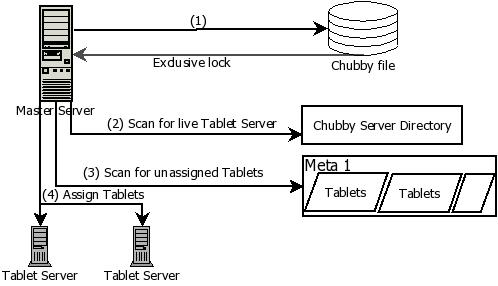
\includegraphics[width=5cm,   height=5cm]{. /figure/random. jpg}
	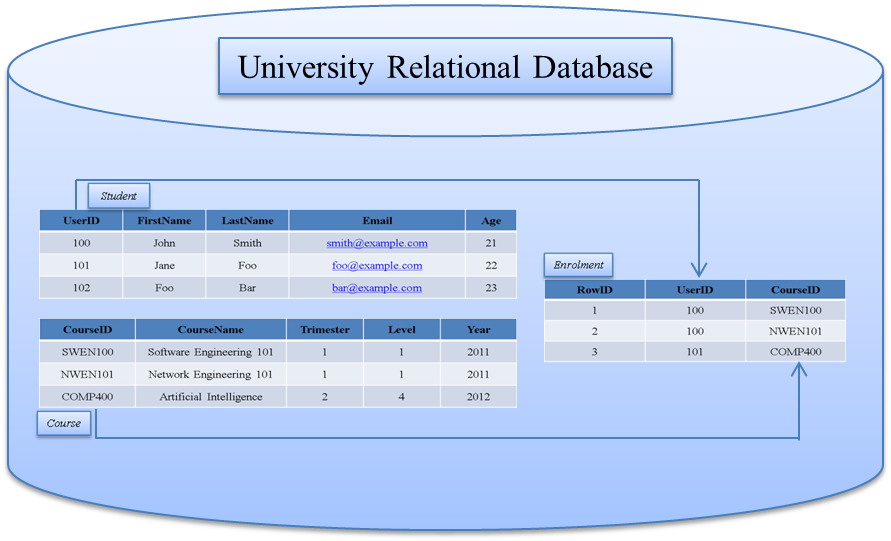
\includegraphics[width=.8\textwidth]{./figure/Example/Relational-DB.png}
	\caption{University example as a Relational database}\label{f:RDB}
\end{figure}

This shows how the University database example is deployed as a
\ac{RDB}.  When data in the University example is modelled using the
column-oriented key-value data model,   the way it is stored is different. 
Although key-value \acp{DBMS} are schema-less,   column-oriented key-value
\acp{DBMS} are not entirely schema-less and hold fewer information about the
constraints within the databases as metadata ,   as seen in Cassandra
(\todo{cite DataStax}).  This data model allows
applications to model the way data is organised in a traditional RDBMS whilst
bringing more flexibility by denormalising data and imposing no rigid structures
or schema requirements (\todo{cite DataStax}).  Therefore,   it allows
applications to add data in the way they want and change their schema (if
needed),   without adhering to a rigid
schema unlike the traditional \acp{RDBMS}.

The building blocks of column-oriented key-value databases are the columns,  
the Super Columns,   the Column Family and the Key Space.  Using the
University example,   these terminologies are explained below. 
Appropriate analogies are drawn with the \ac{RDB} University,   as
seen in Figure~\ref{f:RDB},   to better understand these column-oriented key-value
concepts.  Since the focus is on Cassandra's data model,   these concepts
are explained in the way Cassandra deploys them.  The example used
to describe the Cassandra data model adopts a simple and flexible schema that
allows some structure in the way data is stored. 

\begin{description}
\item[Columns:]  A column is the basic unit of data in this data model.  It is a
tuple containing a column name,   a value and a timestamp (Figure~\ref{f:column}). 

\begin{figure}[h]
	\centering
	%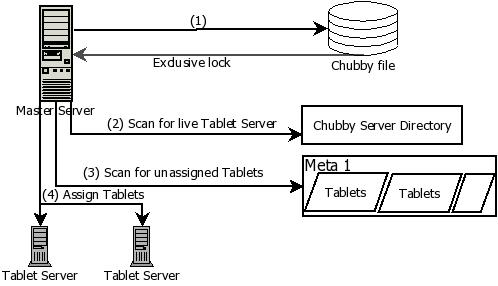
\includegraphics[width=5cm,   height=5cm]{. /figure/random. jpg}
	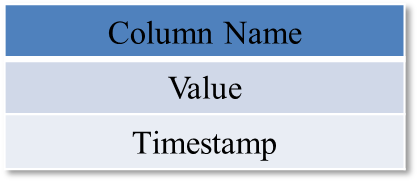
\includegraphics[width=.4\textwidth]{./figure/Example/Column.png}
	\caption{Random Pic}\label{f:column}
\end{figure}

The column names are labels  and it is mandatory that a column has a
name.  Column names and values are stored as Bytes Type,   Long Type,  
Ascii Type,   binary values Lexical UUID Type,   Time UUID Type or as UTF8
serialized strings (\todo{cite }).  Timstamps are used to store the time of the
latest update made to the column and are thus used for conflict resolutions.  The
timestamp values are commonly stored as microseconds,   but could be in any format
that the application chooses.  However,   timestamp formats have to be consistent
across the database so that is the same format across all columns. 

Cassandra allows indexes to be created on column names.  These are called
Secondary indexes and are of type \texttt{Keys} in Cassandra.  When such secondary indexes
are used,   efficient queries can be specified using equality predicates,   and
can be made on ranges of columns too.  The latter ones are called range queries. 

A column name can be considered analogous to a column
in a table in any traditional \ac{RDBMS}.  To illustrate this analogy,
Figures~\ref{f:column-FirstName} and~\ref{f:RDB-User} show the differences
between the representation of values in \texttt{Student} in Cassandra and in an
\ac{RDBMS}.
It can be seen from these figures that a column in the column-oriented key-value
data model is similar to a single value in a row of a relational table.  For
example,   the data '\texttt{John}' in the relational table \texttt{Student} can
be considered equivalent to a single column in Cassandra.

\begin{figure}[H]
	\newcommand{\W}{.4\textwidth}
	\centering
	%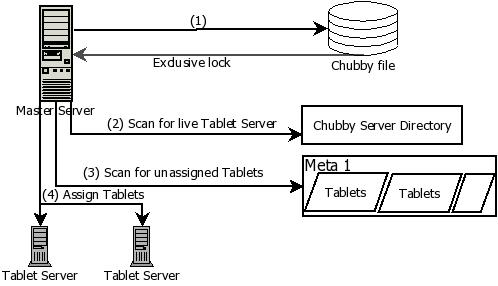
\includegraphics[width=5cm,   height=5cm]{. /figure/random. jpg}
	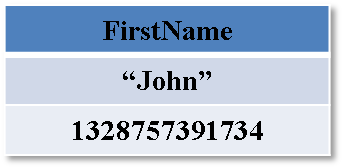
\includegraphics[width=\W]{./figure/Example/Column_FirstName.png}
	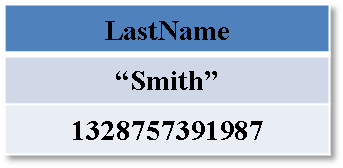
\includegraphics[width=\W]{./figure/Example/Column_LastName.png}
	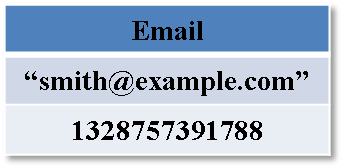
\includegraphics[width=\W]{./figure/Example/Column_Email.png}
	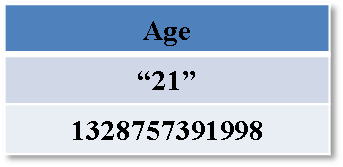
\includegraphics[width=\W]{./figure/Example/Column_Age.png}
	\caption{Columns in Cassandra}\label{f:column-FirstName}
\end{figure}

\begin{figure}[h]
	\centering
	%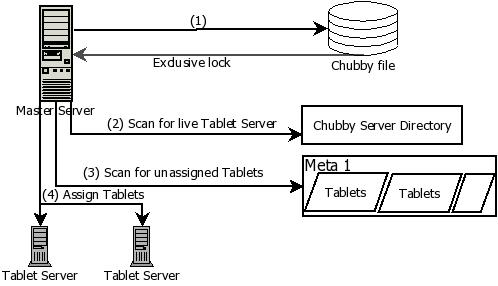
\includegraphics[width=5cm,   height=5cm]{. /figure/random. jpg}
	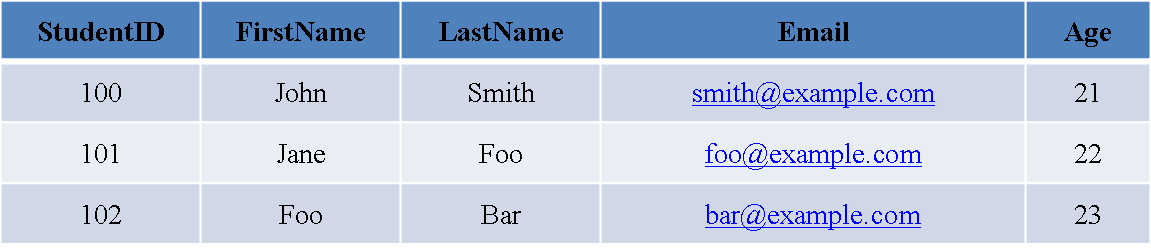
\includegraphics[width=.8\textwidth]{./figure/Example/RelationalTable_User.png}
	\caption{Relational Table - Student}\label{f:RDB-User}
\end{figure}

The JSON notation for  columns in Cassandra is shown in Figure~\ref{f:column-JSON}. 

\begin{figure}[H]
	\centering
	%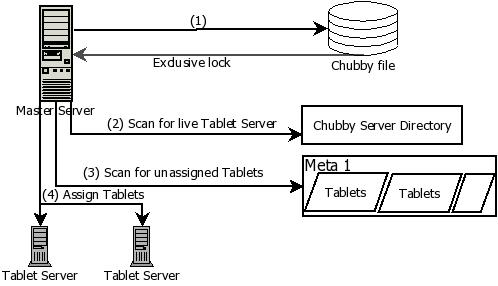
\includegraphics[width=5cm,   height=5cm]{. /figure/random. jpg}
	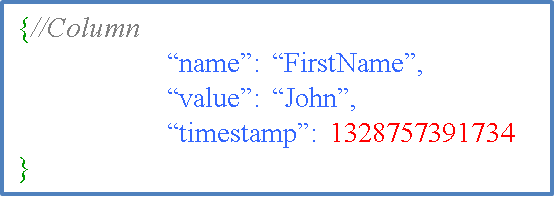
\includegraphics[width=.4\textwidth]{./figure/Example/Column_JSON.png}
	\caption{JSON notation for a column}\label{f:column-JSON}
\end{figure}
% 
% Alternatively,   applications can also use column names to store values.  This is
% possible since it is not required that columns always have values and
% since column names are byte arrays,   applications can store any kind of
% values in it. 

\item [SuperColumns:] A super column is a different kind of a column where the
values are an array of regular columns (Figure~\ref{f:supercolumn}).  It consists of a super
column name and an ordered map of columns.  The columns within the values of a
super column are grouped together using a common look-up value,   which is
commonly referred to as the \texttt{RowKey}.  In other words,   a super column is a
nested key-value pair of columns.  The outer key-value pair forms the super column while the inner
nested key-value pairs are the columns.  Unlike regular columns,   super columns do
not have timestamps for its key-value pairs.  

\begin{figure}[H]
	\centering
	%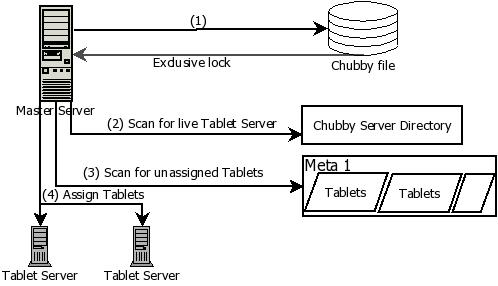
\includegraphics[width=5cm,   height=5cm]{. /figure/random. jpg}
	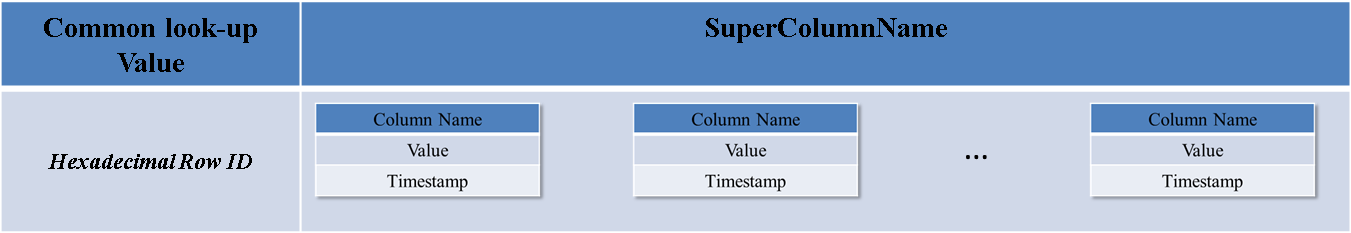
\includegraphics[width=.8\textwidth]{./figure/Example/SuperColumn.png}
	\caption{A Super Column }\label{f:supercolumn}
\end{figure}

A super column can be considered roughly similar to a whole record in a
relational table in an \ac{RDB}. For example,   the super column for a
student,   as seen in Figure~\ref{f:supercolumn-John},   is analogous to a single
record in the relational table \texttt{Student} (Figure~\ref{f:RDB-User}). 

\begin{figure}[H]
	\centering
	%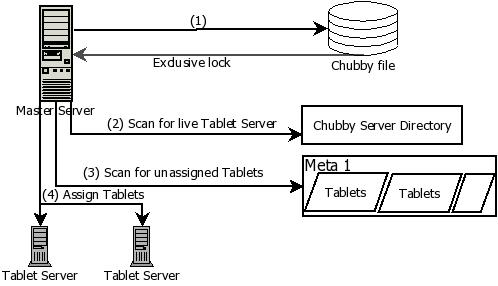
\includegraphics[width=5cm,   height=5cm]{. /figure/random. jpg}
	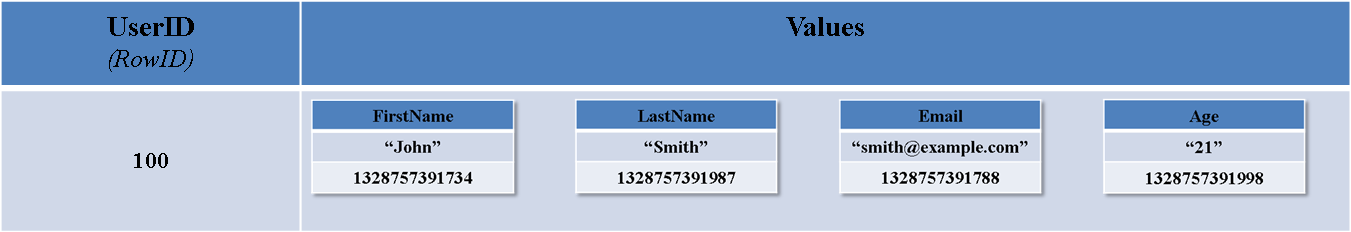
\includegraphics[width=.8\textwidth]{./figure/Example/SuperColumn_John.png}
	\caption{A Super Column for Student '\texttt{John}' in
	Cassandra}\label{f:supercolumn-John}
\end{figure}

The JSON notation for a super column is shown in Figure~\ref{f:supercolumn-JSON}. 

\begin{figure}[H]
	\centering
	%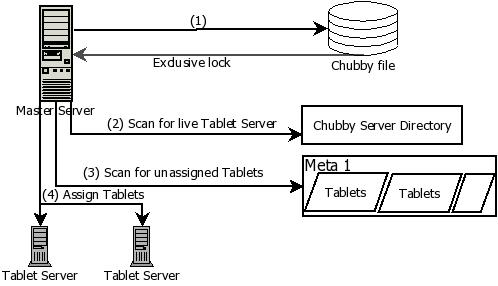
\includegraphics[width=5cm,   height=5cm]{. /figure/random. jpg}
	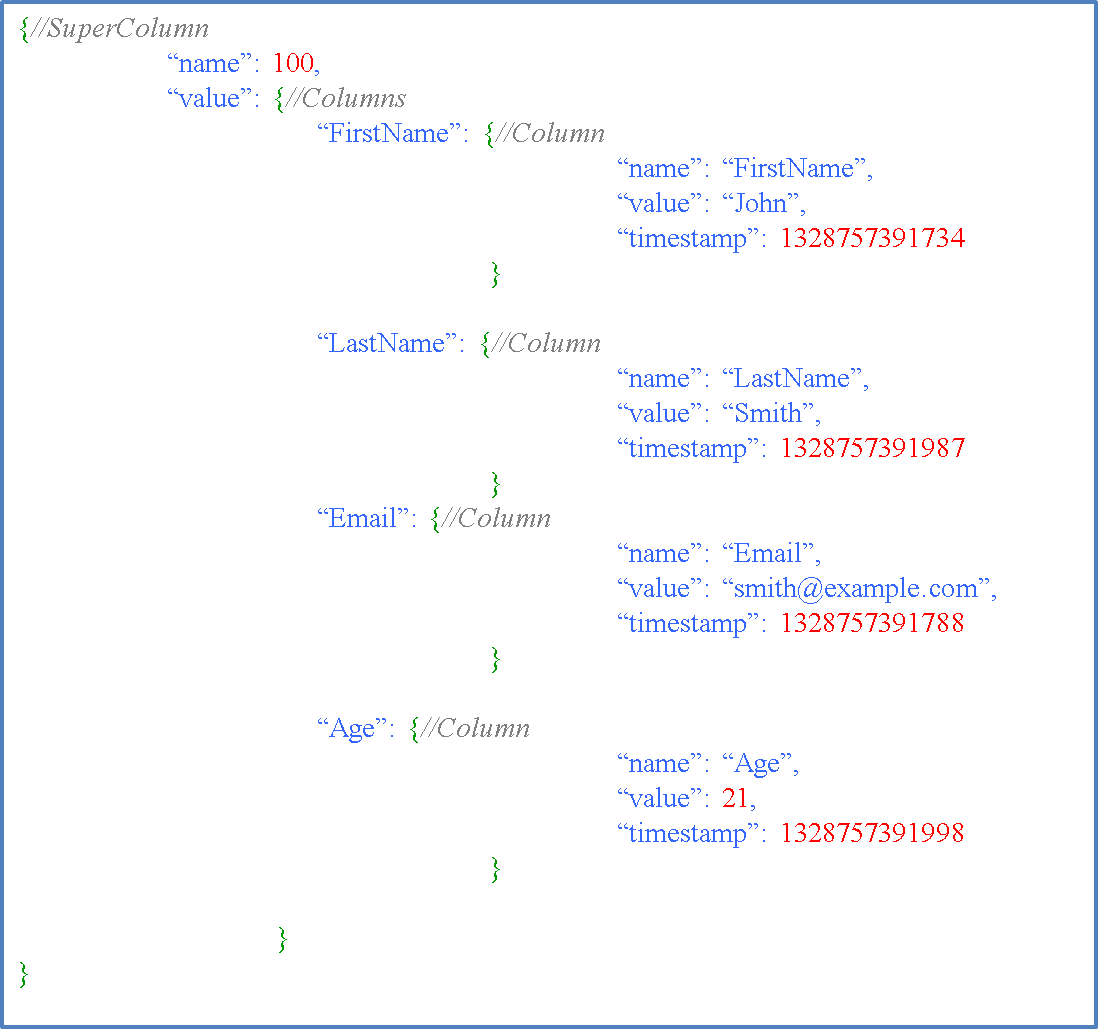
\includegraphics[width=.7\textwidth]{./figure/Example/JSON_SuperColumn_John.png}
	\caption{JSON notation for a super column}\label{f:supercolumn-JSON}
\end{figure}

\item [ColumnFamily:] A column family contains columns or super columns that are
grouped together using a unique row key.  It is a set of key-value
pairs,   where the key is the row key and the value is a map of column names
(Figure~\ref{f:columnfamily}).  The row key groups the columns together,   just as
in super columns. 

\begin{figure}[H]
	\centering
	%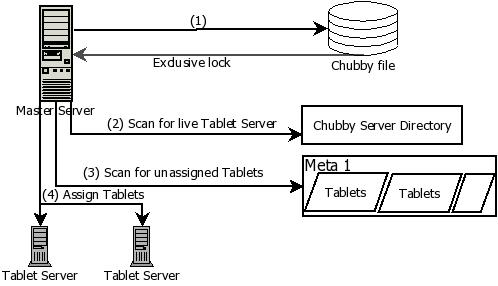
\includegraphics[width=5cm,   height=5cm]{. /figure/random. jpg}
	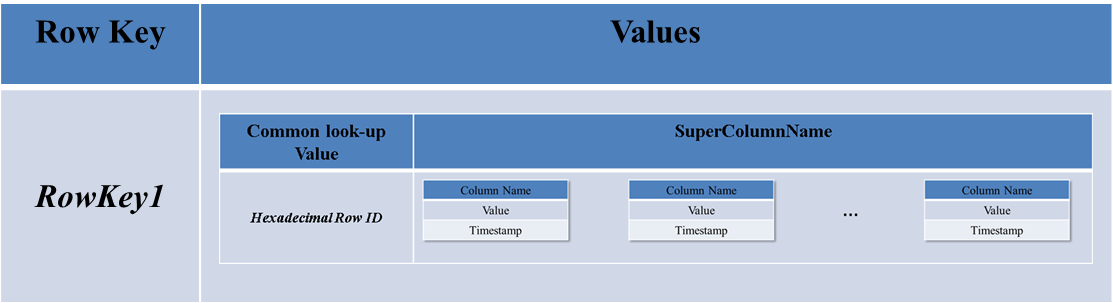
\includegraphics[width=.8\textwidth]{./figure/Example/ColumnFamily.png}
	\caption{Column Family in Cassandra}\label{f:columnfamily}
\end{figure}

Applications can define column families and metadata about the columns. 
It is commonly practised to have columns that are related or accessed
together to be grouped in the same column family.  Column families require that
some attributes are always defined,   like name,   column type and others.  It
also has optional attributes that can be defined if the application requires so.
 Some of the optional attributes are number of keys cached,   comments,   read
repairs,   column metadata among others.

Column families can have rows %to have relatively a definite number of columns. 
that are identified by their unique row keys.  This is similar to a table,   as
seen for table \texttt{Student} in Figure~\ref{f:RDB-User},   where every row in
the table has the same number of columns and primary keys are used to identify a
row.  An example of a column family is shown in Figure~\ref{f:columnfamilyUSER}.
Unlike relational tables in an \ac{RDB},   column families do not require all
the rows to define the same number of columns (\todo{cite Sarkissian}).

\begin{figure}[H]
	\centering
	%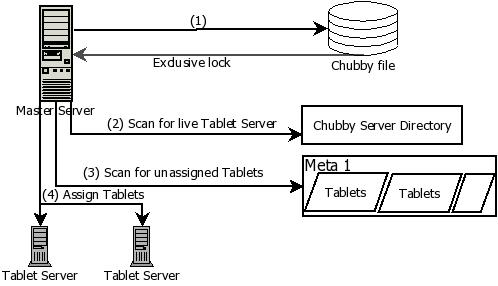
\includegraphics[width=5cm,   height=5cm]{. /figure/random. jpg}
	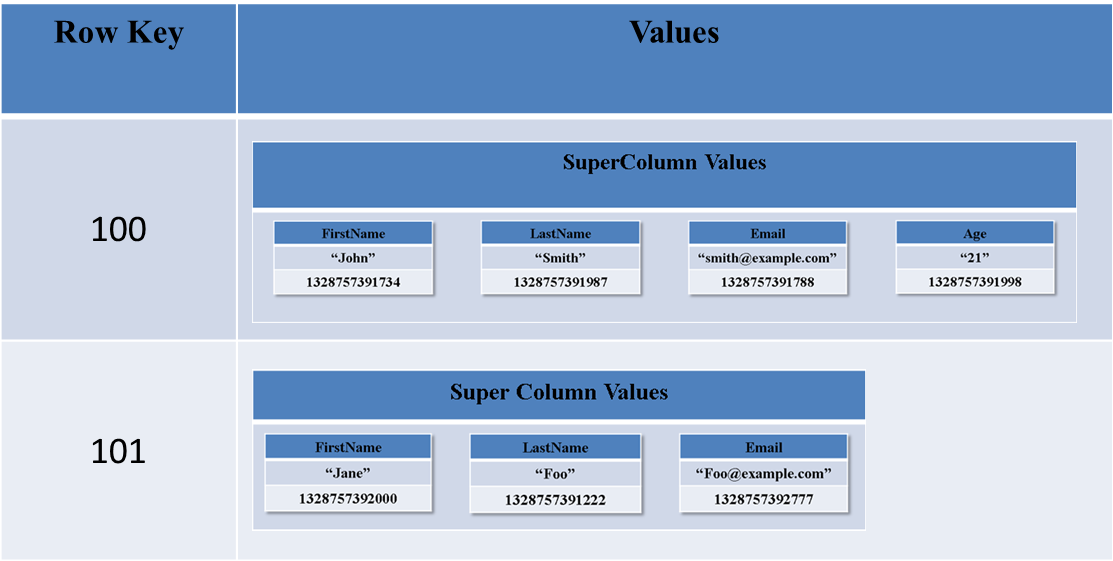
\includegraphics[width=.8\textwidth]{./figure/Example/ColumnFamily-User-DiffColumns.png}
	\caption{Column Family \texttt{User} in Cassandra}\label{f:columnfamilyUSER}
\end{figure}

The JSON notation for a single row of a column family in Cassandra is
shown in Figure~\ref{f:columnfamilyJSON} 

\begin{figure}[H]
	\centering
	%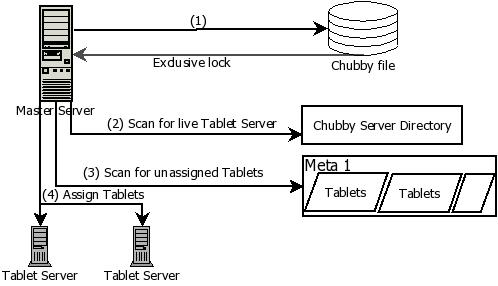
\includegraphics[width=5cm,   height=5cm]{. /figure/random. jpg}
	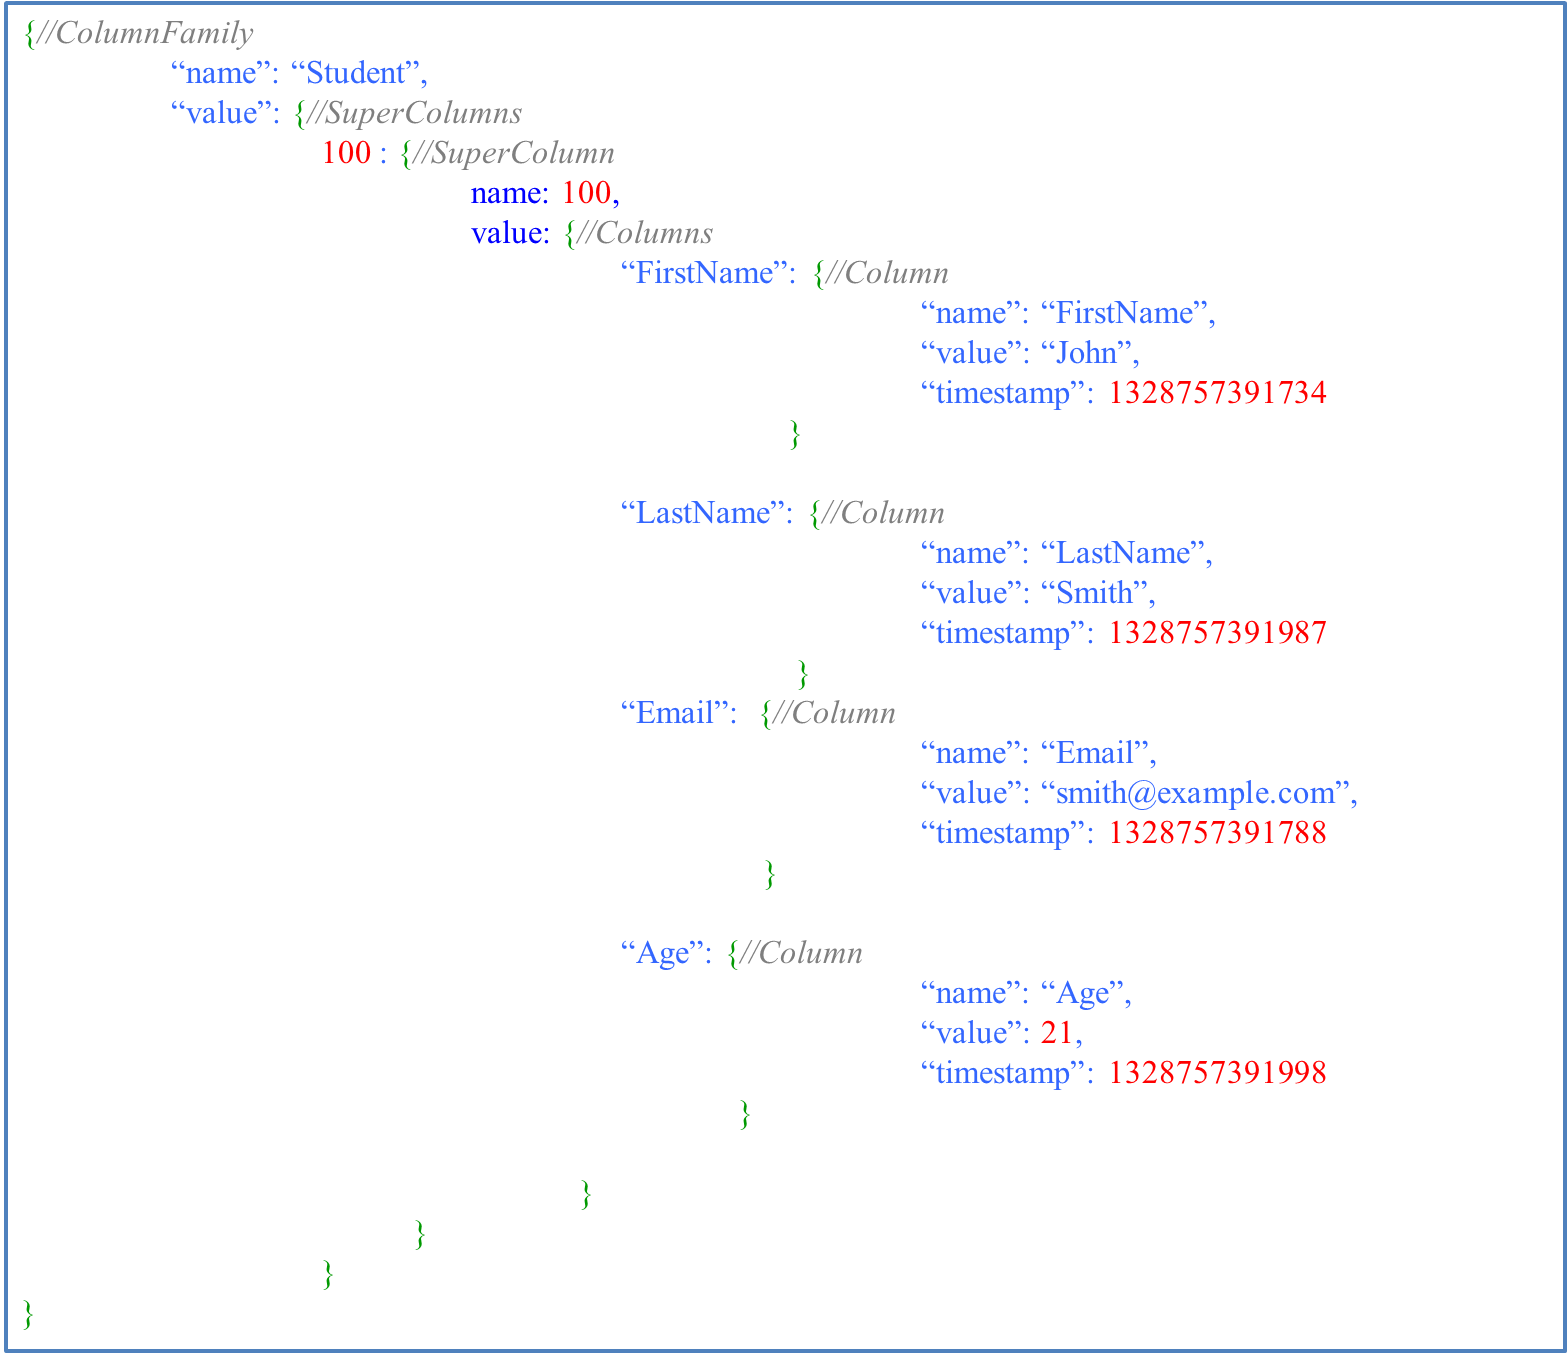
\includegraphics[width=.8\textwidth]{./figure/Example/JSON_ColumnFamily_1row.png}
	\caption{JSON notation for a column family in
	Cassandra}\label{f:columnfamilyJSON}
\end{figure}

\item [KeySpace:] A keyspace is a container to hold the data that the
application uses.  Keyspaces have one or more column families,   although it is not strictly
required that a keyspace should always have column families.  Any relationships
existing between column families in a keyspace are not preserved. 

A keyspace can be considered similar to a database in traditional relational
databases,   without any relationships.  An example of the keyspace
University is shown in Figure~\ref{f:keyspace}. 

Keyspaces require that some attributes are defined,   like a user defined name,  
replication strategy and others.  Some optional elements that can be defined are
the details of the column families in the keyspace and other options
for replication of data. 
\end{description}

%\newpage

\begin{figure}[H]
	\centering
	%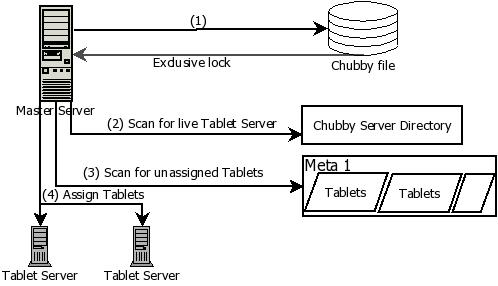
\includegraphics[width=5cm,   height=5cm]{. /figure/random. jpg}
	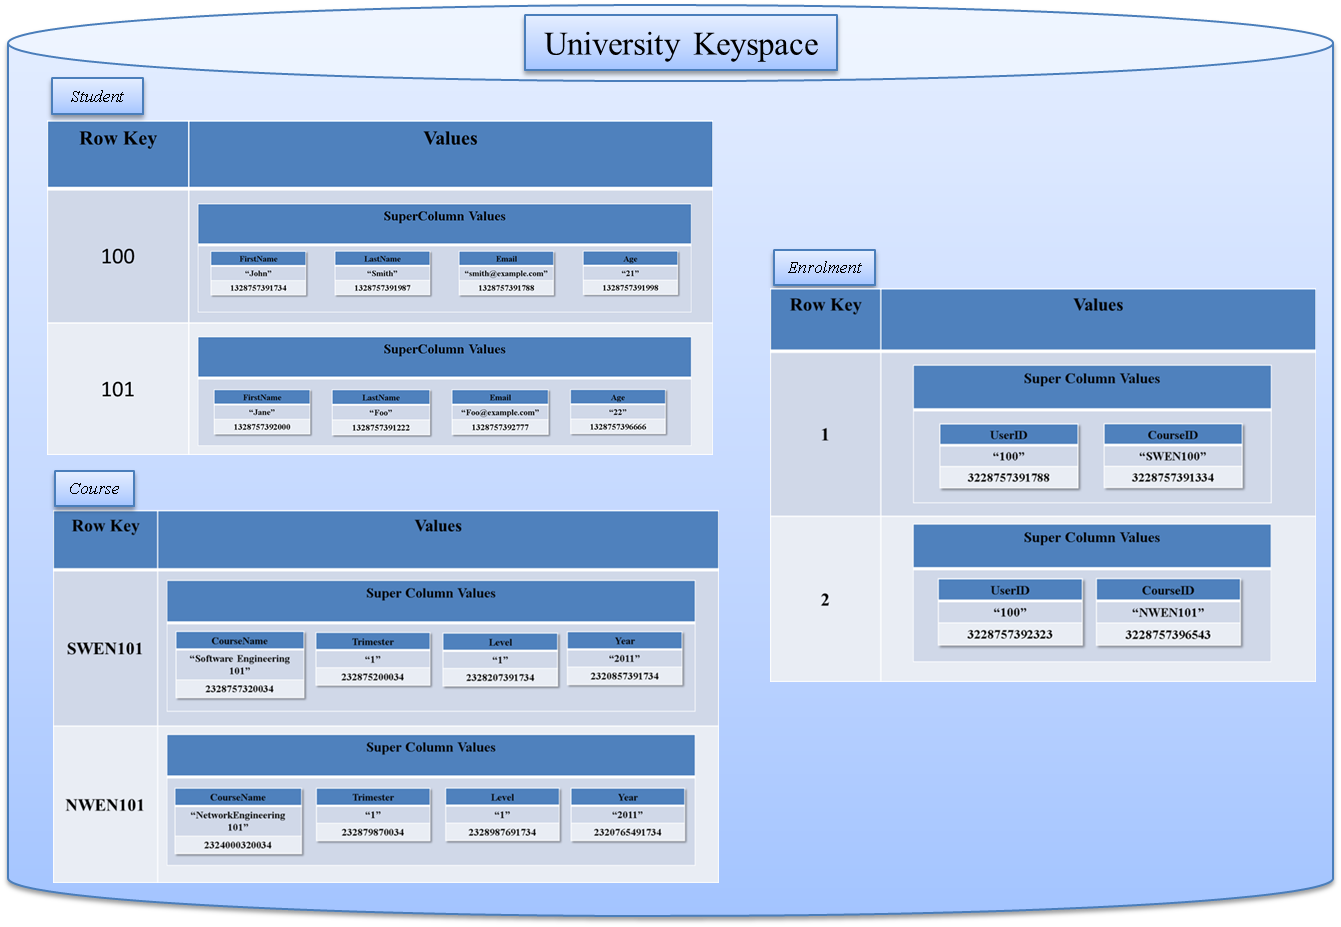
\includegraphics[width=.9\textwidth]{./figure/Example/KEYSPACE.png}
	\caption{A keyspace in
	Cassandra}\label{f:keyspace}
\end{figure}

As previously mentioned,  cloud \ac{NoSQL}
\acp{DBMS} are generally specialised to address specific problems like
partition-tolerance,  high availability among others and for this some
trade-off are made when these are developed.
Some of the challenges and problems present in such \acp{DBMS} are discussed in the following section.

\section{Challenges in Key-Value model}\label{s:challenges-key-value}
Fundamentally,   the key-value data model is different from the relational model
in many ways.  While the relational data model aims at giving data a structure,  
providing data integrity,   the key-value data model just
store data as \acp{blob} or string values and generally do not maintain
relationships between data.  In the column-oriented key-value model,   the
key-value association and the grouping of columns in column families can be
considered as the minimum relationship that is maintained.  

According to Bell and Brockhausen (1995),   data dependencies are the most
common types of semantic constraints in relational databases and these determine
the database design.  Data dependencies are the various relationships that may
exist between data entities in a database.  For example,   in the
University database,   a student can enrol into more than one course and this
means that there is a many-to-many relationship between \texttt{Student} and
\texttt{Course} since   one course can have many students enrolled in it.  

As seen in Section~\ref{s:key-value-data-model},   the \texttt{Enrolment} table 
contains the \texttt{StudentID} and the \texttt{CourseID} as foreign keys,  
thus showing the dependency or relationship between students and courses
(Figure~\ref{f:RDB}). 
In the \texttt{University} \ac{RDB} any attempt to delete a course
from the \texttt{Course} table,   is prevented by a constraint,   unless the
dependency itself is removed first.  In \acp{RDBMS} ,   this constraint is referential
integrity,   which ensures that references between data entities are valid,  
consistent and intact (\todo(cite Blaha,   n. d. )). 
Normalisation,   as well as modelling real world data and
relationships enforce such dependencies in the schema and this causes integrity
constraints like referential integrity constraints,   to be imposed on data
entities. 

If such constraints are not imposed,   there could arise many dangling
dependencies in the database.  For instance,   consider the case of foreign key
references between \texttt{Course} and \texttt{Enrolment} in the  University
database.  If a course is deleted from the \texttt{Course} table without removing
its dependencies in \texttt{Enrolment},   the latter would contain active references
to the deleted course.  Another example of a dangling reference occurs during
insertion of data,   where a new student is entered in the
\texttt{Enrolment} table,   with a \texttt{CourseID},   that does not
exist in the \texttt{Course} table (i. e. ,   wrong \texttt{CourseID}).  A dangling
reference occurs because this inserted student refers to a nonexistent course. 
Such problems cause inconsistent data to be stored in databases and violate data
integrity.  To ensure that users get consistent and valid information,  
applications would have to implement mechanisms to check or prevent dangling references.  But if
referential integrity constraints are applied as in an \ac{RDB},   operations
on data that  adversely affects referential integrity   would not be
permitted.

As previously mentioned,   \ac{NoSQL} database systems do not normalise data and
nor are any relationships maintained.  But relationships or dependencies
between data are common when real world data is stored in databases.  For example,   in the
real world,   a course could be taught by more than one lecturer or a student with
an Art major is restricted entry into Chemistry courses etc.  These relationships
and constraints have to be preserved upon storage in
cloud \ac{NoSQL} database systems too.  As mentioned in
Section~\ref{s:cloud-databases},   cloud databases,   whether relational or
\ac{NoSQL},   have to replicate data across several machines and need to be
scalable to match the needs of the users.  The replicated and distributed nature
makes maintaining data dependencies complex and unfeasible in terms of speed and
efficiency.  In cloud \ac{NoSQL} databases,   this effectively means that the
relationship between \texttt{Enrolment}, \texttt{Student} and \texttt{Course}
tables will not be strictly enforced and deleting a course in cloud \ac{NoSQL} databases is allowed because
of the absence of constraints.  As mentioned before,   this means that students
could still be enrolled in deleted courses,   since there are no constraints to
prevent such deletions or changes in cloud \ac{NoSQL} databases. 

Commonly,   developers impose such constraints and reference checks on \ac{NoSQL}
data at the application side.  Another way to implement such checks is to give
these constraints at the persistence layer of the application server.  Both these
ways would eventually have to handle all the processing and managing of these
constraint checks for all the widely spread data in \ac{NoSQL} databases. 
However,   this could mean immense workload on the application or the application
server,   especially if the data volume is large in the \ac{NoSQL} database or if it is
has many replicas that have to be checked as well for the constraints. 


This is a serious problem when data is interconnected and dependant on other
data entities as is commonly the case.  For example,   consider a banking
application that uses cloud \ac{NoSQL} \acp{DBMS} where its data is spread
across several nodes and is interconnected.  Any debit or credit
transactions made to a users account will have to be replicated across all the
nodes and correctly persisted.  Many constraints will exist for transfer of funds
between user accounts and such constraints need to be validated correctly.  If a
user has multiple accounts,   the relationship between the accounts have to be
maintained too.  When such constraints are not validated correctly,   it will lead
to incorrect account balances and wrong updates in the user accounts.  On the
other hand,   when such applications use an \ac{RDBMS},   referential integrity
constraints would be imposed to maintain the relationships between the
accounts and such constraints would be defined while tables are created and
their validation would be triggered whenever any operations are performed on the
data. 

Updates may not be correctly reflected across all the nodes of the database due
to  eventual consistency too,   which is discussed in Section~\ref{s:Cassandra}. 
However, in spite of eventual consistency,   data dependencies should be correctly handled and
recorded. 

Although such problems mostly affect most cloud \ac{NoSQL} \ac{DBMS} users,   it
could be different for different users.  For example,   a banking system as
mentioned above could be gravely affected because of dangling references while
in a simple game application such problems could be trivial. 

% Motivated by such problems of data dependencies,   this thesis studies the
% existing modelling of data dependencies in cloud \ac{NoSQL} database systems and
% aims to contribute by suggesting four solutions so that referential integrity
% is effectively maintained,   while also not limiting the benefits of not having
% a rigid schema in \ac{NoSQL} database systems.  Such a result would reduce the
% workload of the applications or the persistence layers of the application
% servers.  Additionally it would give users of \ac{NoSQL} database systems
% better consistency in data,   along with ensuring better data integrity even when
% it is widely replicated or spread on different data-centers. 



\section{Referential Integrity in Key-Value
Model}\label{s:referential-integrity}
Addressing the aforementioned challenges,   implies to introduce referential
integrity constraints in cloud \ac{NoSQL} database systems. 

Referential integrity is a fundamental property of data within databases,   which
ensures that data dependencies between tables are maintained correctly in the
database (\todo{cite oracle}).  These dependencies could be a part of the
business rule and need to be enforced for proper data integrity.  Users define
conditions or rules on the tables in a database so that data integrity is
ensured at all times.  These conditions are called integrity constraints and need
to be mandatorily satisfied at all times in order to ensure that users or
applications do not enter incorrect or inconsistent data into the databases. 

The Referential Integrity Constraint is just one amongst other constraints,   and
generally in \acp{RDBMS},   these constraints ensure that the value of foreign
keys in a table matches the values of primary keys in another table.  The table
containing the foreign key is the referencing table (or child table),  
while the table with the primary or unique key is the referenced table (or parent table). 
For example,   in the University database,   \texttt{Enrolment} is the
referencing table while \texttt{Student} and \texttt{Course} are the
referenced tables.  Foreign keys are also known as the referencing key and
the primary keys as the referenced keys. 

It has been defined by many researchers that referential integrity is enforced
by the combination of a primary (or unique) key and a foreign key,   and that
every foreign key has to match the primary key (\todo{cite}).  In the
University example,   every foreign key in the \texttt{Enrolment} table must match
one of the primary keys in the \texttt{Student} and \texttt{Course} tables. 
Hence,   if any foreign key refers to a non-existing primary key,   the
referential integrity constraint is violated.   For example,   if
'\texttt{StudID100}' is a foreign key for a student in the \texttt{Enrolment}
table,   but '\texttt{StudID100}' does not exist as a primary key in the \texttt{Student}
table,   then it is a violation of referential integrity. 
 
Referential integrity constraints also describe the data manipulation that is
allowed on the referenced values.  Some of the widely associated rules are:

\begin{itemize}
  \item \texttt{Restrict} or \texttt{No delete}: which prevents any update or
  deletion of data that has references. 
\item \texttt{Set to NULL}: which sets all foreign keys to NULL values,   on
updating or deleting the referenced key. 
\item \texttt{Set to Default}: which sets all the foreign
keys to a default value,   on updating or deleting the referenced key. 
\item \texttt{Cascade}: which updates or deletes all the
associated dependant values accordingly,   when the referenced data is updated or
deleted. 
\item \texttt{No Action}: which performs checks only at the end of a
statement and is similar to \texttt{Restrict}
\end{itemize}

Existing \acp{DBMS} may not always support all of the above rules.  Some \acp{DBMS} may
have the \texttt{Cascade} rule by default like Oracle,   while some may have the
\texttt{Restrict} rule by default.  

Generally,   in \acp{RDBMS} the database manager enforces a set of rules to
prevent nay data operation,   like insert,   update or delete,   to change data in
such a way that referential integrity is not violated as seen in
Figure~\ref{f:RI}. 

\begin{figure}[H]
	\centering
	%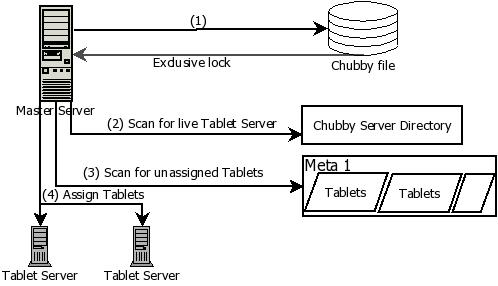
\includegraphics[width=5cm,   height=5cm]{. /figure/random. jpg}
	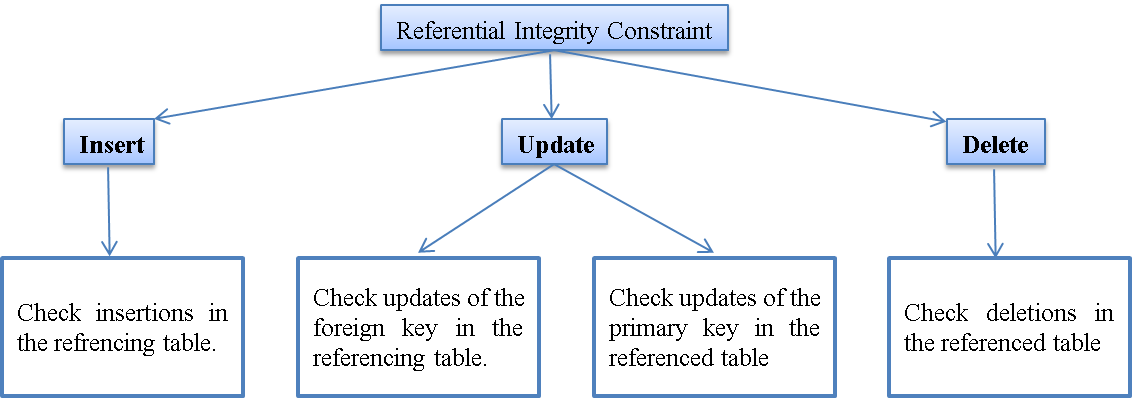
\includegraphics[width=.8\textwidth]{./figure/Example/RI-Figure.png}
	\caption{Referential Integrity Rules}\label{f:RI}
\end{figure}

These rules are explained below:

\begin{itemize}
  \item Insert rule: An insert operation triggers a referential integrity
validation when data is being inserted into a referencing table,   i. e. ,   the
child table.  In such an event,   prior to entering the values in the referencing
table,   it is checked if the foreign keys exist in the referenced table.  For
example,   in the University \ac{RDB},   when a row is inserted in the
\texttt{Enrolment} table with foreign key values for \texttt{StudentID} and
\texttt{CourseID},   a check is triggered to verify whether these foreign keys
exist in the \texttt{Course} and \texttt{Student} tables as primary keys.  If
the foreign keys do not exist in the referenced tables,   then the insert operation is not allowed. 

\item Update rule: When data is updated either in the referencing table or
the referenced table,   a referential integrity validation is needed.  When any
primary key is updated in the referenced table,  
then it is verified whether this key is a foreign key in any of the
referencing tables.  If a dependency is found to exist,   then the applicable
data manipulation rule is checked.  For instance,   if it is a \texttt{Cascade}
rule,   then the associated foreign keys in the referencing table are updated
prior to updating the key in the referenced table.  In the University \ac{RDB},  
if the primary key '\texttt{SWEN100}' for a course is updated to
'\texttt{SWEN101}',   then all the records in \texttt{Enrolment} that have
'\texttt{SWEN100}' as a foreign key have to be updated to '\texttt{SWEN101}',  
if it has a \texttt{Cascade} rule. 

When any foreign key is being updated in a referencing table,   then a referential
integrity validation has to be performed.  It is ensured that the new
updated value exists as a primary key in the referenced table.  For example,   in
the \texttt{Enrolment} table,   if \texttt{CourseID} in a row is updated to a new
value,   then it is verified that the new value is an existing primary key in the
\texttt{Course} table.  If the new value does not exist,   the
update is not allowed generally. 

\item Delete rule: A delete operation triggers a referential integrity
validation when data is deleted from the referenced table.  When data that is marked
for deletion is found to have dependencies in other referencing tables,   the
data manipulation rule applicable for this operation has to be checked.  This
means that if the rule allows \texttt{Cascade},   then the depending values in the
referencing table have to be removed prior to deleting values from the
referenced tables.  For example,   when a student record is deleted from the
\texttt{Student} table,   a check is performed to see if the '\texttt{StudentID}'
is a foreign key in any other table.  Therefore,   \texttt{Enrolment} would be
checked and when the '\texttt{StudentID}' is found as a foreign key,   the
appropriate action is performed depending on the data manipulation rule.  If it
is '\texttt{Cascade}',   the enrolment details for the '\texttt{StudentID}' are
removed from \texttt{Enrolment} and then the student record is deleted from
\texttt{Student}. 

\end{itemize}

Referential integrity constraints have been a relational feature in traditional
\acp{RDBMS} and is imposed due to the way the \acp{RDBMS} enforce normalisation. 
To improve the data dependency in cloud \ac{NoSQL} \acp{DBMS},   this
thesis proposes solutions that implement referential integrity constraints using
different approaches. These solutions implement and
validate referential integrity constraints based on these fundamental data manipulation and
referential integrity rules and are discussed in Chapter 3.

% These proposed solutions are deployed and analysed in Cassandra,  which is a
% column-oriented key-value \ac{DBMS}. To implement any solution it is necessary
% to understand the architecture and the key operations allowed in a \ac{DBMS}.
% For this purpose,  the architecture of Cassandra is discussed in the following section.



\section{Summary}



This chapter presented the background about the underlying concepts in cloud
computing and cloud databases.  It is clear that cloud computing is gaining
prevalence due to its many benefits like high data availability and cheap
storage etc.  With an increase in the number of users
migrating to cloud computing,   cloud data storage is gaining prominence as well,  
for easy and simple data storage.  This has paved the way for the existence
of many different data models and databases on the cloud.  Amongst the many data
models,   the key-value data model has been  most widely used  on the cloud
as it is more adapted to the cloud environment due to its support for
replication and scalability and other cloud related features (\todo{cite}). 



The next chapter describes the four solutions proposed to enforce referential
integrity constraints in cloud \ac{NoSQL} \acp{DBMS},   particularly in
Cassandra which is based on the column-oriented key-value data model. 






% \acresetall
% %ब
\chapter{Solutions for Referential Integrity Constraints in NoSQL
databases}
\label{c:solutions}

% As mentioned previously,  cloud column-oriented key-value \acp{DBMS} lack
% referential integrity constraints to maintain foreign key relationships,  as
% seen in traditional \acp{RDBMS},  due to its non-relational data model. 
% Moreover,  these cloud \acp{DBMS} do not normalise data nor maintain
% relationships.
Traditionally, referential
integrity constraints are imposed on data items of a database to maintain
foreign key relationships. These relationships are
 maintained by correctly identifying and preserving the data dependencies 
 existing between the data items.
% Traditionally, foreign key relationships are
% maintained by correctly identifying and preserving the data dependencies existing between data items in a database.
% These dependencies are maintained and  validated by imposing referential
% integrity constraints on data items. 
Most popular traditional \acp{RDBMS}
preserve such dependency information in their \texttt{System} tables or data
dictionaries.  These tables store the necessary information  which is required
to maintain valid dependencies. The information stored in such tables include table
names,  primary and foreign keys among others.
This can be seen in popular \acp{RDBMS} like  MS SQL Server,  PostgreSQL,
Oracle, and so on.  

For example,  in MS SQL Server 2000, \texttt{sysforeignkeys}
is a \texttt{System} table which stores the information of all 
foreign keys of every table in a database, and \texttt{sysreferences}
stores the mappings of  foreign keys to the referenced primary key columns
(\todo{\citep{sys:msdn}}).
Information in these \texttt{System} tables consist of  the
names of tables and its constraints,  unique identifiers of 
referenced and referencing columns,  among others. 
In PostgreSQL, such information is saved as views which contain the dependency
information of data items in a database.
The view \texttt{table\_constraints} contains the information for all the
constraints in every table owned by the current user. (\todo{\cite{}}). 
Similarly, Oracle uses a \texttt{SYSTEM} meta-database to hold such constraint
information.
 In general, \texttt{System} tables or views with information
about the existing dependencies  are looked up by these \acp{DBMS} whenever
referential integrity checks are triggered \citep{sys:msdn}.


The solutions presented in this chapter save the dependency information as
metadata. This metadata contains relevant  information about  foreign
key relationships in keyspaces \todo{J:and more stuff, right?}, and it is
accessed whenever an operation is performed on the data and referential
integrity needs to be validated. 


This chapter describes  four  solutions  that implement referential
integrity constraints in a cloud \ac{NoSQL} \ac{DBMS}.
Section~\ref{s:Metadata} describes the metadata used by the solutions 
 to store the depency information.
Section~\ref{s:API} describes the design and implementation of the experimental
API developed to integrate all the four
solutions. 
Section~\ref{s:sol1} describes  the first solution, which implements
referential integrity constraints by saving metadata along with the actual data.
Section~\ref{s:sol2} describes the second  solution where metadata is
saved as a top row. Section~\ref{s:sol3} describes the third   
solution which saves metadata separate from the actual data.   
Section~\ref{s:sol4}  describes the fourth solution which saves metadata in a separate cluster.
Finally, Section~\ref{s:solutions-summary} presents a brief summary of this
chapter. 

\section{Metadata}\label{s:Metadata}
Metadata in \acp{DBMS} provide information about the data stored. It may
contains details related to schemas, constraints,  primary and foreign keys, and
so on.   As previously mentioned,  most traditional \acp{RDBMS} maintain such
metadata within their \texttt{System}  tables or data dictionaries.  
In Apache Cassandra, the \ac{DBMS} of interest, metadata is stored in a 
keyspace named \texttt{System} and it contains information
about the cluster and its nodes along with information related to the
keyspaces, column families, and so on (\todo{cite BOOK}).
 Even when Cassandra has a  \texttt{System} keyspace to store metadata, it 
 is read-only and hence it cannot be modified to store additional metadata
 about referential integrity constraints. 
%  As
% previously mentioned ,  most traditional \acp{RDBMS}
% maintain such metadata within their \texttt{System} tables or data dictionaries.
% Such metadata is decoupled from the actual data and its operations,  so that
% retrieving the metadata is faster since it does not involve handling the actual
% data(\todo{cite Duval}). 
% It has been studied that the \ac{DaaS} is moving towards maintaining metadata in
% the cloud \acp{DBMS},  where commonly this metadata stores information about the
% nodes in a distributed cluster (\todo{cite Bin(2010)}).  For  maintaining the
% scalability required in such cloud \acp{DBMS}, metadata is often decoupled from
% the actual data so that accessing metadata does not cause a bottleneck in
% performance.  Cassandra maintains  metadata about the nodes in a
% cluster  in a separate keyspace named \texttt{System}, which stores the
% properties of every node, for example the node tokens,  the name of the
% cluster to which  nodes belongs to, information about the stored keyspaces and
% column families and so on(\todo{cite BOOK}). 
% As per the design of Cassandra,  the \texttt{System} keyspace cannot be modified
% and thus  the metadata for the   solutions cannot be incorporated in this
% \texttt{System} keyspace.  Hence,  for preserving the metadata in each 
% solution implements a  different strategy In other words, metadata is associated
% with actual data in different ways.  Associations can be classified as
% (\todo{cite Duval}):
Hence,  for preserving the metadata, each 
solution implements a  different strategy in which metadata is associated
with actual data. Solutions~1 and~2 use embedded metadata, that is, metadata
is created with the actual data; while solutions~3 and~4
associate metadata separately from the actual data.  Notice that, the structure
 of the metadata is kept the same across all the solutions even when  the way of
 storing and associating this metadata is different in each. 

The role of metadata in  the solutions is primarily to hold the necessary
 information required to maintain referential integrity. The metadata contains  
 information about primary keys,   foreign keys,  referenced and referencing
 column family details, constraints, and others.  The constraints considered in
 the solutions can be either \ac{PK} or \ac{FK} 
constraints. \ac{PK}
constraints specify which column is the primary key of a column family, while 
\ac{FK} constraints (or referential integrity constraints) determine the
foreign key relationship between two column families, that is, the
 column of a column family that  is dependent on the primary key  column of
 another column family.  Hence, for each column family with a primary key,  the
metadata  contains one \ac{PK} constraint  and  as
many \ac{FK} constraints as foreign key relationships. 
% Notice that, throughout
%  the solutions, the structure of metadata containing these constraints is
% consistent despite.  

The structure of the metadata is shown in
Figure~\ref{f:metadataInSolutions}.  This structure contains information about
a University keyspace example\todo{Where is the example defined?}. In this
 example, a simple schema is applied for the keyspace where  the details of the
 students are saved in  the \texttt{Student} column family and the course
 details in the \texttt{Course} column family. 
 The enrolment details of students are saved in the 
\texttt{Enrolment} column family by associating students to courses and
hence having foreign key relationships to both  column families. All the column
families have unique primary keys and their \ac{PK} constraints are saved in
the metadata as presented in Figure~\ref{f:metadataInSolutions}, while the
foreign key relationships between \texttt{Enrolment}, \texttt{Student} and
\texttt{Course} are saved as \ac{FK} constraints.  For instance, consider in
 Figure~\ref{f:metadataInSolutions} the \ac{PK} constraint \texttt{CONST100},
 for the \texttt{Student} column family, and the \ac{FK} constraint  
 \texttt{CONST400} for the foreign key relationship between
\texttt{Enrolment} and \texttt{Student}.

\begin{figure}[h]
	\centering
	
	\newcolumntype{C}{@{\hspace{2.5pt}}>{\scriptsize}c@{\hspace{2.5pt}}}
	\begin{tabular}{CCC CCC CC}
		\toprule
		\bfseries ConstraintName & \bfseries Keyspace & \bfseries ConstraintType &
		\bfseries ColumnFamily & \bfseries RKeyspace & \bfseries RConstraintName &
		\bfseries RColumn & \bfseries DeleteRule\\
		\midrule
		CONST100 & University & P & Student & University & & StudentId &\\
		\rc CONST200 & University & P & Course & University & & CourseId &\\
		CONST300 & University & P & Enrolment & University & & RowId &\\
% 		\hline
% 		\hline
		\rc CONST400 & University & F & Enrolment & University & CONST100 & StudentId
		& CASCADE\\
		CONST500 & University & F & Enrolment & University & CONST200 & CourseId &
		NODELETE\\
		\bottomrule
	\end{tabular}
	\caption{Metadata for the Solutions}\label{f:metadataInSolutions}
\end{figure}


Specifically, the structure of the metadata contains:

\begin{itemize}
  
  \item \texttt{ConstraintName:} is the name assigned for
  every constraint and it uniquely identifies an
  existing \ac{PK} or \ac{FK} constraint in the metadata. 
   For example,  \texttt{CONST100} and \texttt{CONST400} are the
  \texttt{ConstraintNames}.
  
  \item \texttt{Keyspace:}represents the name of the Keyspace the constraint
  belongs to. 
  
  \item \texttt{ConstraintType:} denotes the type of the constraint and the
  possible values are '\texttt{P}'.and '\texttt{F}'.
  The former referes to  a \ac{PK} constraint while the latter represents  a
   \ac{FK} constraint. 
   
  \item \texttt{ColumnFamily:} refers to the column family this constraint
  exists in. For example,  the \ac{PK} constraint
  \texttt{CONST100}  exists in column family \texttt{Student} and the column
  family of the \ac{FK} constraint \texttt{CONST400}
  is \texttt{Enrolment}.
  
  \item \texttt{RKeyspace:}is the name of the keyspace on which this constraint
  is applied.  In the example, constraints  are applied in  the keyspace
  \texttt{University}.
  
    
  \item \texttt{RConstraintName:} For a \ac{FK}
  constraint,  \texttt{RConstraintName} represents the name of the
  referenced \ac{PK} constraint . In other words, it indicates which primary key
  is referenced. In the example,  the \ac{FK} constraint \texttt{CONST400}
   references the \ac{PK} constraint \texttt{CONST100},  which means that
   \texttt{Enrolment} has a foreign key relationship with \texttt{Student}.
   Notice that in a \ac{PK} constraint  this field is left blank since it
   has no references to other keys.
  
  \item \texttt{RColumn:}  indicates the primary key column on which this
  constraint is applicable.  For \ac{PK} constraints,  this holds the name of
  the primary key column. For \ac{FK} constraints, this field denotes
  the referenced column.  This example shows that the \ac{PK} constraint
  \texttt{CONST100} is applied on the primary key column \texttt{StudentId} of
  \texttt{Student} column family . The \ac{FK} constraint \texttt{CONST400}
  shows that the referenced column is \texttt{StudentId},  indicating that
  \texttt{Enrolment} references  primary key column \texttt{StudentId} of
  \texttt{Student}.
  
  \item \texttt{DeleteRule:}stores the type of data manipulation rule applicable
  on this constraint. The possible values are  \texttt{Cascade} and
  \texttt{NoDelete}.  This field is not applicable  for \ac{PK} constraints
   since data manipulation rules are associated with constraints that hold
  dependency information like the \ac{FK} constraints.
  
\end{itemize}

Metadata in the solutions are accessed whenever referential integrity
validations are triggered to extract information about \ac{FK} constraints. 
Specific methods are designed in all the solutions to retrieve and process the
metadata in order to validate referential integrity.  These methods and all the
solutions are incorporated  into an experimental \ac{API}, which is
described in the following section.

\section{Experimental API}\label{s:API}

The experimental \ac{API} is designed generically in order to ensure
that it can be used by  applications to maintain dependencies within their
keyspaces irrespective of keyspace schemas or structures of column
families. However, applications using this \ac{API}  have to provide
 the metadata information relevant to the constraints of their keyspace as
 explained in the previous section. 
% Thus,  this \ac{API} is made adaptable to different keyspace schemas  that can
% be deployed in column-oriented key-value \acp{DBMS}.  

This \ac{API} validates the referential integrity based on the metadata provided
for the application and its column families.  It  provides  four solutions
with different approaches to meet different requirements. However, with 
 every one of these solutions,  the referential integrity constraint is
 implemented in Cassandra.

The  class diagram of the \ac{API} is presented seen in
 Figure~\ref{f:classDiagram} alongside with the example classes that belong to 
the University keyspace. The main components are the Entities, Entity Managers,
and Validation handlers, all of which are described in the next sections.  
 Notice that for the sake of clarity and brevity,  the class diagram only
 contains  the relevant  methods of the classes, favoring a simpler
explanation of the functioning of the \ac{API}.

\begin{figure}[h] 
	\centering
	%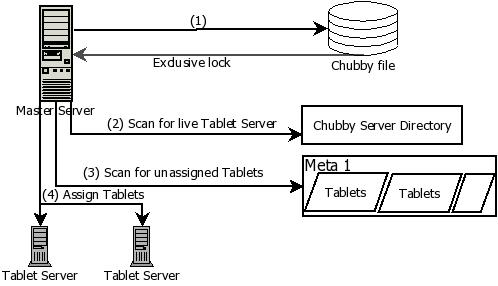
\includegraphics[width=5cm,   height=5cm]{. /figure/random. jpg}
	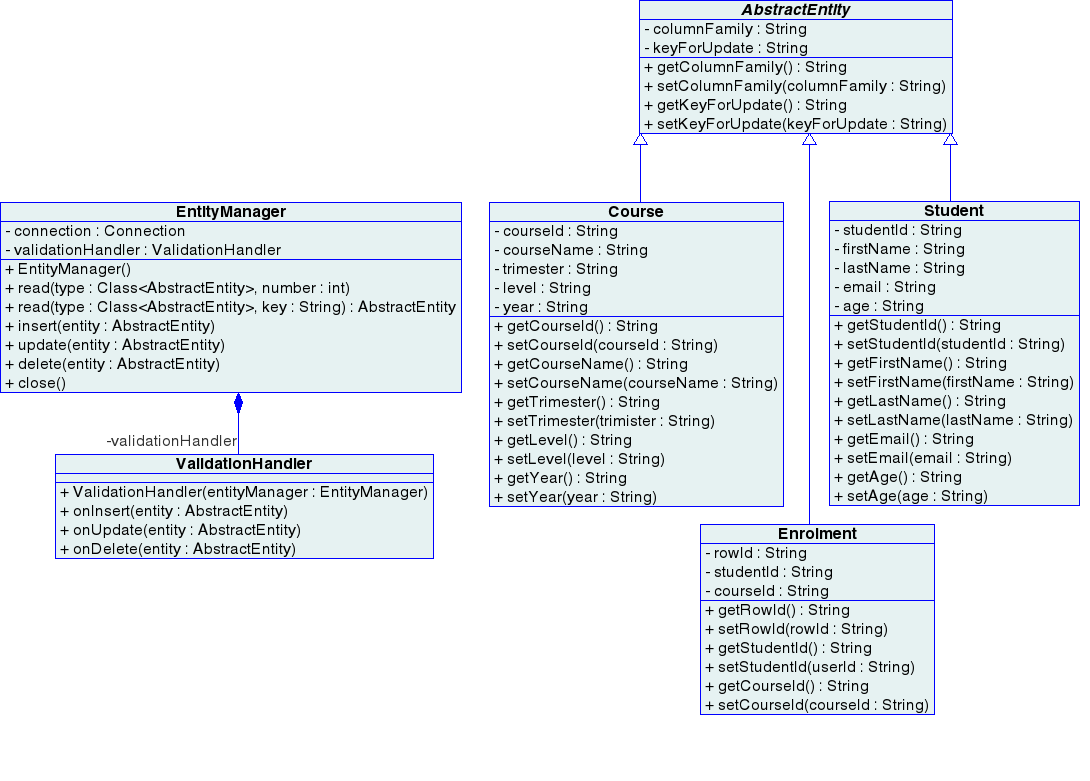
\includegraphics[width=\textwidth]{./figure/Solutions/FinalClassDiagram.png}
	\caption{Class Diagram for the \ac{API}}\label{f:classDiagram}
\end{figure}


	\subsection{Entities} 
	\todo{add attributes of AbstractEntity!!!}
	An entity class contains attributes (with respective getters and setters) that
	map columns within a specific column family. As such, the contents of a
	column family can be represented by a list of entity objects. All entities in
	the \ac{API} extend from the abstract class \texttt{AbstractEntity} which
	contains attributes (and respective getters and setters) to
	aid the \ac{API} towards their management. Particularly, the attributes
	that \texttt{AbstractEntity} contains  are \texttt{columnFamily} which
	determines the column family to which the entity maps, and 
	\texttt{keyForUpdate} which shall contain the new value in case the primary key
	of the entity is to be updated.
	
	For example,  considering the University keyspace example, \texttt{Enrolment} 
	is an entity class that  maps the \texttt{Enrolment}  column family and
	it contains the attributes \texttt{RowId}, \texttt{CourseId} and
	\texttt{StudentId} which represent the respective columns. As such, an instance
	of \texttt{Enrolment} contains the values of one super column. Likewise,
	\texttt{Student} and \texttt{Course} are entity classes which instances 
	map to their respective super columns in their column families.
% 	For all the solutions in this \ac{API},  entities of the user applications are
% 	designed to extend the abstract class called \texttt{AbstractEntity},  which has
% 	information about the  methods for accessing and defining  entities.  For
% 	every column family, applications derive a class from the
% 	\texttt{AbstractEntity} containing attributes.
	The \ac{CRUD} operations that can be performed on these entities   are
	handled by the \texttt{EntityManager},  which is described next.
		
	\subsection{EntityManager}

	The  \texttt{EntityManager} class implements  all
	the \ac{CRUD} operations to be performed on the entities. In order to perform
	these operations,  the \texttt{EntityManager} interacts with the respective
	keyspace the entity belongs. Moreover, it ensures to trigger the   referential
	integrity validation process whenever a \ac{CRUD} operation requires it. This
	is performed by creating a  \texttt{ValidationHandler} (explained in the next
	section) and passing the entity to be checked for constraint violations. 
	
	The \texttt{EntityManager}, before performing any operation, requires a
	connection to the keyspace. This connection is established using a third-party
	\ac{API} named Hector (freely available at \todo{www.hector.com}). Hector
	 encapsulates the driver-level interface provided by Cassandra (named Thrift) 
	 and simplifies the interaction with it. Regarding the \ac{CRUD} 
	 operations, Hector provides  a \texttt{Mutator} object which encapsulates the
	 necessary procedures to interact with the Cassandra cluster.    
	 
	 Notice that  the \texttt{EntityManager} is able to generically deal with any
	 entity that derives from \texttt{AbstractEntity}. It does so by using
	 reflection (a Java  feature) to detect the attributes of an object and
	 generically invoking the getters and setters of the entities. Thus, the
	 \texttt{EntityManager} is able to perform all \ac{CRUD} operations on
	 any entity. These operations are explained in detail next.  
	 
	 
	
% 	Hector is a high
% 	 level client that wraps the driver-level interface of Cassandra called Thrift.
% 	 Hector  provides some features that  Thrift does not, for example, 
% 	 fail-over mechanisms and connection pooling (\todo{cite book}).  
	 % 	 While there
% 	 are other wrappers for Thrift, Hector was  chosen as  it is one of the
% 	 earliest wrappers and  encapsulates the interaction with the Thrift \ac{API}
% 	 and makes it simpler to access a Cassandra cluster.	
	
	
	
	
		\subsubsection{Create}
		 The \texttt{create} (or \texttt{insert}) operation stores entities in the
		 respective column families. The \texttt{EntityManager} inserts these entities
		into the column families represented by the entity class.  
		For example,  all the student entities are inserted into the column family
		\texttt{Student} through the \texttt{EntityManager}. 
		
		The \texttt{EntityManager} passes the entity details which include entity key
		and column family information as parameters to the \texttt{addInsertion}
		method of the \texttt{Mutator}.  The \texttt{insert} operation triggers a
		 referential integrity validation whenever a child entity is  inserted in
		 order to ensure that its parent entities exist. The validation is performed
		 by the \texttt{onInsert} method of \texttt{ValidationHandler}, which is
		explained in Section~\ref{ss:VH}.
	
		\subsubsection{Read}
		The  \texttt{read} operation retrieves  entities from a keyspace given the
		entity class. This operation does not prompt any referential integrity validation since
 		entities are only read and their state is not changed, unlike in the other
		operations.
		
		\todo{talk about mutator CONSISTENCY}
		
		This \ac{API} provides two methods for retrieving entities. One retrieves a
		single entity given its class and the value of the respective primary key. The
		other retrieves a list of entities representing the contents of
		the column family.

		
		
		\subsubsection{Update}\label{ss:update}
		In an \texttt{update} operation the existing contents of an entity are merged
		with new contents.  In other words, the  values of their columns they
		represent are updated to new values and committed into the column families.  
		 The \texttt{EntityManager} provides two types of updates, one in which it
		 uses the primary key of the entity to update it, and the other one in
		 which uses the especial field \texttt{keyForUpdate} to update the primary as
		 well as the rest of the fields. 
		 
		 If the entity to be updated does not contain a change in its primary key, a
		 normal update takes place. Otherwise, referential integrity needs to be
		 ensured. In order to do so, the following steps are performed:
% 		 In order to do so, the \texttt{EntityManager} passes the entity
% 		 to the \texttt{ValidationHandler}  to check for referential integrity, 
% 		 retrieves the list of child entities that depend on its primary key, deletes
% 		 dependencies and the entity,  and update the dependencies Following this, the
% 		 steps that are performed are :
		\begin{enumerate}
		  \item Check with the \texttt{ValidationHandler} if the entity can be
		  updated.
		  \item Retrieve the list of child entities that depend on the previous
		  primary key of the entity to be updated.
		  \item Perform \texttt{delete} on the child entities from their column family
		  in Cassandra.
		  \item Perform a \texttt{delete} on the entity with the primary key from the
		  column family.
		  \item Perform an \texttt{insert} with the entity and its new primary key.
		  \item Update the foreign keys in the child dependencies to
		  the new value.
		  \item Perform an \texttt{insert} operation to reinsert the child entities
		  into their respective column families.
		\end{enumerate}
		
% 		In all the solutions,  an \texttt{Update} operation triggers a referential
% 		 integrity validation whenever any primary or foreign keys of any entities are
% 		updated.
% 		The validations are performed by the \texttt{onUpdate} method of the
% 		\texttt{ValidationHandler}.
		
		Notice that such procedure is used as a workaround of the restriction of
		Cassandra to change a primary key. Once a record has been
		inserted into the column family, the primary key cannot  be changed. This is
		known as a tombstone delete, which prevents aside from changing a primary
		key, deleting a primary key.
		
		\subsubsection{Delete}\label{ss:delete}
		In a  \texttt{Delete} operation, entities are removed from a column
		family. As mentioned before, due to the tombstone delete, the primary key
		will never cease to exist, but the values of the columns are emptied. 
		
		In all the solutions,  a \texttt{Delete} operation triggers a referential
		integrity validation every time a parent entity is deleted.  This validation
		is performed by the \texttt{onDelete} method of the
		\texttt{ValidationHandler}, which is explained in next section. 
		 
		 The 	\texttt{EntityManager} passes the entity information to the
		\texttt{delete} method of the \texttt{Mutator} object.
 		
%  		Before a parent entity is deleted, the \texttt{EntityManager} retrieves the
%  		child entities it depends upon  from he \texttt{ValidationHandler} if the
%  		 referential intergity is not violated. The \texttt{EntityManager} deletes
%  		the child entities prior to deleting the parent entity.
		
		\subsection{ValidationHandler}\label{ss:VH}
		The \texttt{ValidationHandler} is invoked by the \texttt{EntityManager} every time
		an operation triggers a
		referential integrity validation on any entity. 
		The \texttt{EntityManager} passes the entity and the connection details  to
		the \texttt{ValidationHandler} to perform the validation.
		
		The \texttt{ValidationHandler} contains the  logic for checking whether an
		 entity has any dependencies and verifies whether an \texttt{insert},
		 \texttt{update} or \texttt{delete} operation  violates the referential
		integrity or not.  To ensure that these operations maintain referential
		 integrity between entities, it applies the appropriate referential integrity
		 rules, as explained in Section~\ref{s:referential-integrity}. Thus, for an
		 \texttt{insert} operation the insert rule of referential integrity is
		 followed and similarly for \texttt{update} and \texttt{delete} operations
		 their respective rules are applied. As previously mentioned, a \texttt{read}
		 operation does not invoke any refreential integrity validation in this
		 \ac{API}. The referential integrity validation performed by
		 \texttt{ValidationHandler} for each of these operations is discussed next
		with pseudocodes.
		
		\begin{description}
		\item[onInsert]: 
		In an \texttt{insert} operation a referential
		integrity validation is triggered whenever a child entity is  inserted. 
		The \texttt{ValidationHandler} applies the referential integrity insert
		rule which checks whether  valid parent entities with
		primary keys matching the foreign keys of the child entities exist, else an
		exception is raised stating that the referential integrity has been violated.
		The implementation of the \texttt{insert} operation is consistent across all the
		solutions. 
		\todo{Insert Pseudocode}
		
		\item[onUpdate:] The validation for an \texttt{update} operation is different
		when primary keys and foreign keys are updated. 
		\begin{description}
		\item[Case A: Update Primary Key] When a  primary key of a
		parent entity is updated, the \texttt{ValidationHandler} performs the
		following checks.
		\renewcommand{\labelenumii}{\arabic{enumi}.\arabic{enumii}}
		\renewcommand{\labelenumiii}{\arabic{enumi}.\arabic{enumii}.\arabic{enumiii}}
		%\renewcommand{\labelenumiiii}{\arabic{enumi}.\arabic{enumii}.\arabic{enumiii}.\arabic{enumiiii}}
		\begin{enumerate}
		  \item if \ac{FK} constraints on primary key exist
		  	\begin{enumerate}		  	
		    \item if \texttt{DeleteRule} for the \ac{FK} constraint is
		    \texttt{Cascade}
		    	\begin{enumerate}
		    	  \item Pass any existing child entities to the \texttt{EntityManager} to
		    	  allow update of both parent and child entities.
				\end{enumerate}
			\item else if \texttt{DeleteRule}  is \texttt{NoDelete}
				\begin{enumerate}
				  \item if no child entities exist
				  		\begin{enumerate}
				  		  \item \texttt{EntityManager} performs update on  the primary key
				  		\end{enumerate}
				  \item else if child entities exist
				   		\begin{enumerate}
				    	\item Raise exception and rollback \texttt{update}. 
				    	\end{enumerate}
				\end{enumerate}
			\end{enumerate}
		  \item else if no \ac{FK} constraints are found 
		  		\begin{enumerate}
		  		  \item \texttt{EntityManager}
		  performs update on the primary key
				\end{enumerate}
		 \end{enumerate}
		 
		For example,  in the University keyspace,  when a
		new \texttt{StudentId} is provided for an existing  \texttt{Student}
		entity,  then \texttt{ValidationHandler}
		checks metadata and locates the \ac{FK} constraint \texttt{CONST400} as seen in
		Figure~\ref{f:metadataInSolutions}. Since the \texttt{DeleteRule} is
		\texttt{Cascade}, the \texttt{EntityManager} allows the \texttt{update}
		operation to take place as explained in the EntityManager section.
			
% 			For example, when the foreign key \texttt{StudentId} for one of the entities
% 		in \texttt{Enrolment} is given a new value,  then the \texttt{ValidationHandler} 
% 		identifies the parent entity class for its \ac{FK} constraint
% 		\texttt{CONST400} as \texttt{Student}.  If the new \texttt{StudentId} 
% 		exists as a primary key for any
% 		 of the  entities in \texttt{Student} entity class,  the \texttt{update} is
% 		 performed.
		 
		\item[Case B: Update Foreign Key] When a foreign key of a child entity is
		updated, the  \texttt{EntityManager} performs the same check on the
		metadata and locates its parent entities. It then follows these steps:
		\begin{enumerate}
		  \item Identify parent entity class from the \ac{FK} constraint
		  \item if new foreign keys exist as primary key in parent entity class
			\begin{enumerate}
				\item \texttt{EntityManager} updates  the foreign key
			\end{enumerate}
		  \item else 
			\begin{enumerate}
				\item Raise exception
			\end{enumerate}
		\end{enumerate}

	
		
		\end{description}
		The implementation of the \texttt{update} operation for both the cases is
		consistent for all solutions.
		
		\item[onDelete:] In a \texttt{delete} operation a referential
		integrity validation is triggered whenever an entity is deleted. The
		\texttt{ValidationHandler} applies the referential integrity delete rule
		and performs the following checks:
		\renewcommand{\labelenumii}{\arabic{enumi}.\arabic{enumii}}
		\renewcommand{\labelenumiii}{\arabic{enumi}.\arabic{enumii}.\arabic{enumiii}}
		
		\begin{enumerate}
		  \item Identify existing \ac{FK} constraints on the entity.
		  \item if \ac{FK} constraints exist,
		  		\begin{enumerate}
		  		  \item if \texttt{DeleteRule} is \texttt{Cascade}
		  		 		\begin{enumerate}
		  		 		   \item Pass any existing child entities to the \texttt{EntityManager}
		  		 		   to allow delete of child  and parent entities.
		  		 		\end{enumerate}
		  		  \item else if \texttt{DeleteRule}  is \texttt{NoDelete}
						\begin{enumerate}
						  \item if no child entities exist
						  		\begin{enumerate}
						  		  \item \texttt{EntityManager} deletes the entity.
						  		\end{enumerate}
						  \item else if child entities exist
						   		\begin{enumerate}
						    		\item Raise exception  
						    	\end{enumerate}
						\end{enumerate}
						
				  \item else if no \ac{FK} constraints are found 
				  		\begin{enumerate}
				  		  \item \texttt{EntityManager} deletes the entity
						\end{enumerate}
		  		\end{enumerate}
		\end{enumerate}	
		For example,  in the University keyspace,  if a 
		\texttt{Student} entity in \texttt{Student} column family is marked for
		deletion, the \texttt{EntityManager} locates the \ac{FK} constraint 
		\texttt{CONST400} referencing \texttt{Student}.
		Since the \texttt{DeleteRule} is \texttt{Cascade}, 
		the child entities are deleted from \texttt{Enrolment} prior to deleting the
		entity from its \texttt{Student} column family. 
		\end{description}
		
% 		
% 		Since metadata is stored differently in the solutions, the operation for
% 		retrieving the metadata in the  \texttt{ValidationHandler} is different for
% 		each solution in the \ac{API}. 
% 		 For example,  the \texttt{ValidationHandler}
% 		for Solution 1 and 2 involves parsing the metadata  since it is stored as a
% 		 \texttt{String} along with the actual data while in Solution 3 and 4 it is
% 		 saved as an entity class.
% 		
% 		The implementation,  connection settings and operations 
% 		are common for all the solutions in the \ac{API}.  
% 		The following sections describe the solutions,  the motivation for the
% 		solution's design and the way the solutions save metadata. 
		
	
\section{Solution 1:  Metadata with Special Characters}\label{s:sol1}

	
	The first solution saves
	metadata as the value in a key-value pair  in
	column-oriented key-value \acp{DBMS} .
	The solution proposes saving the dependency information of the entities as
	metadata and including it in the entity's value.  In this solution, the
	different parts of the metadata
	are separated by the special character '\texttt{,}'.
	To achieve this in a column-oriented key-value \ac{DBMS}, the metadata is saved
	as a part of each of the super column  in a column family.
	In every super column,  this metadata is separated from its columns
	 by storing the metadata surrounded with curly brackets. For example,  in the
	 University keyspace example,  the column family of \texttt{Student} saves
	 the metadata as a part of the value  for every  super
	 column in it (Figure~\ref{}).

%|ConstraintName:CONST200;KeySpace:UNIVERSITY;ConstraintType:P;TableName:harsha_thesis_api_solution2_entity_Course;RKeySpace:UNIVERSITY;RConstraintName:;RColumn:CourseId;DeleteRule:|;
% |ConstraintName:CONST600;KeySpace:UNIVERSITY;ConstraintType:F;TableName:harsha_thesis_api_solution2_entity_Enrolment;RKeySpace:UNIVERSITY;RConstraintName:CONST500;RColumn:CourseId;DeleteRule:NODELETE|;

	For this solution,  the different parts of the metadata is
	accessed by the \texttt{ValidationHandler}  to determine whether the entity has
	any dependencies. The different parts of the metadata is parsed by the
	\texttt{BaseEntity} and each constraint in the metadata is handled as a
	\texttt{String} and the special characters '\texttt{\{}',  '\texttt{, }' and
	'\texttt{\}}' become the delimiters for parsing the \texttt{String} and
	splitting it into tokens. Thus, each of these tokens
	would hold one of the parts of the constraint. For example, the metadata for
	\texttt{Student} entity will be parsed into tokens where one token will
	contain the value of \texttt{ConstraintName} \texttt{CONST100}, while another
	will contain the \texttt{Keyspace} value \texttt{UNIVERSITY} and likewise all the
	parts of the constraint will be tokenised. Thus, the \texttt{ValidationHandler} accesses the tokens to determine the various parts fo the metadata. For example, to determine the \texttt{DeleteRule} for a
	\ac{FK} constraint the \texttt{ValidationHandler} would read the respective token.

	The logic for the referential integrity validation by the
	\texttt{ValidationHandler} once the \texttt{String} metedata is parsed is the
	same as described in Section~\ref{ss:VH}.

	In this solution, the metadata is saved  when entities are inserted into the
	column family and thus the metadata is a part of each of the entity.  Since the
	metadata is present as the value in every super column,  accessing the metadata
	information for referential integrity validation is as simple as accessing the
	value itself,  requiring no additional actions or connection to the
	keyspace. Saving the metadata as embedded metadata in this solution is useful
	as entities are replicated across the distributed cluster, making metadata
	easily accessible by every node in the cluster, since it is a part of the
	entity.
	
	The \ac{API} parses the metadata of an entity by reading any of its 
	instances and need not load metadata from any external location.

	On the other hand,  the metadata for an entity would be the same for all its
	instances .  For example,  in the University example,  the metadata
	information for the \texttt{Student} entity is applicable to each of its
	instances,  indicating that each instance  should have a primary key called
	\texttt{StudentID}.
	Similarly,  all \texttt{Course} instances have the same \ac{PK} constraints
	applied on it.  When metadata is saved as a part of the  value,
	every instance of an entity will contain the constraint information
	in it's value.  Since the metadata information and constraints are same for all
	the instances of a single entity ,  this metadata is repeated every time an
	instance of the entity is inserted.  For example,  if
	\texttt{1000} \texttt{Student} instances are inserted,  the metadata for these
	\texttt{1000} instances are saved \texttt{1000} times too, along with these
	instances.  But the metadata is exactly same for all the
	instances \todo{(Figure~\ref{})}.


	The distributed nature of cloud \ac{NoSQL} \acp{DBMS} also means that the
	metadata is not only repeated several times within the same column family,  but
	also across the nodes in the cluster, thus increasing the redundancy of
	the metadata.  But such a redundancy and consumption
	of space to store the metadata is not a potential issue
	in cloud column-oriented key-value \acp{DBMS}, since storage on the cloud is
	inexpensive and  does not affect the economic benefits.

	Such a storage mechanism is not expected to affect the efficiency of the
	cluster negatively as the metadata information is not large in size and is
	easily replicated along with the actual data and does not exert any extra
	resources in the cluster.  The performance of this solution is analysed  in
	Chapter~\ref{}.

	Much research has been done in the area of  metadata management in distributed
	environments,  where emphasis is laid on the synchronous updates of metadata
	storage as well as its efficient storage and access mechanisms(\todo{cite more}
	Hackl et al.  2010).
	In Hackl et al.  (2010),  metadata management is discussed in the context of
	huge file systems, where metadata is stored separately in a suitable \ac{DBMS}
	so that such file systems can be managed and administered efficiently without
	slowing them down.  To analyse which type of \ac{DBMS} was more suitable for such a
	metadata storage,  they conducted various experiments and concluded that
	key-value \acp{DBMS} were more efficient in terms of speed,  memory and resource
	consumption when compared to popular \acp{RDBMS}.  As a part of their
	experiments, they adopted an interesting approach to store metadata in a
	key-value \ac{DBMS} ,  namely Tokyo Cabinet,  a popular \ac{NoSQL} \ac{DBMS}
	that stores records as simple key-value pairs in data files. Unlike Cassandra,
	tokyoCabinet does not involve data types or columns
	and so on (\todo{cite}).  In their approach,  metadata about the file system
	used in their experiment is inserted as a value which is associated with a unique key and the
	different parts of the metadata are separated by semicolons (Hackl et al.  2010).
	
\section{Solution 2:  Metadata as Top Row}\label{s:sol2}



\section{Solution 3:  Metadata Tables}\label{s:sol3}



\section{Solution 4:  Metadata Clusters}\label{s:sol4}

\section{Summary}\label{s:solutions-summary}
Mention limitaitons
%  \section{Limitations}\label{s:lim}
% Transaction
% cascade on one level of nesting
% unique or composite keys
% school network  -->  experimental design





% 
% \acresetall
% \chapter{Experimental Design}
\todo{Check number of enrolments, introduce all metadata, and retrieve 
details of cassandra cluster from my computer}

\todo{summary of chapter structure}


\section{Benchmark keyspace}
In order to asses the performance of Cassandra when the four solutions are
executed, the experimental \ac{API} is implemented by loading
 entitites that belong to a University keyspace. The University keyspace is
designed for the experiments to store the details of students and courses
belonging to a university along with the enrolment details of the students.The
class diagram for the University keyspace is shown in
Figure~\ref{fexp:ClassDiagram}. The entities are saved as the following column
families in Cassandra.

	\begin{itemize}
	  \item \texttt{Student} to store the student attributes which are its primary
	  key \texttt{StudentId}, \texttt{FirstName}, \texttt{LastName},
	  \texttt{Email} and \texttt{Age}
	  \item \texttt{Course} to store course information where the attributes are
	  its primary key \texttt{CourseId}, \texttt{CourseName}, \texttt{Trimester},
	  \texttt{Level} and \texttt{Year}
	  \item \texttt{Enrolment} to preserve the relationship between students and the
	  courses they enrol into. The attributes for \texttt{Enrolment} are its
	  primary key \texttt{RowId}, \texttt{StudentId} and \texttt{CourseId}
	\end{itemize}
	


	\begin{figure}[h] \centering
		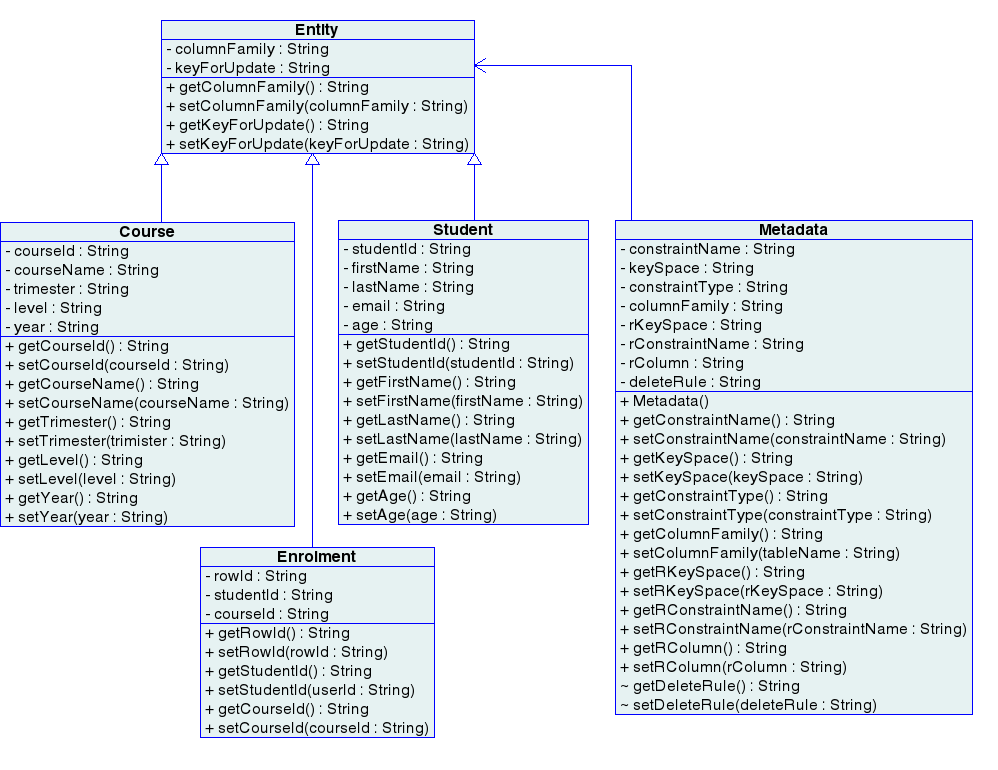
\includegraphics[width=1\textwidth]{./figure/Solutions/classdiagram-experimental.png}
		\caption{Class Diagram for University}\label{fexp:ClassDiagram}
	\end{figure} 

The constraints for the keyspace is stored in the \texttt{Metadata} entity.
These constraints are the \ac{PK} and \ac{FK} constraints applicable on each of
the column families in this keyspace. The list of constraints are the same for
all the solutions  and are shown in Table~\ref{texp:ListConstraints}.



\begin{table}[h] \label{texp:ListConstraints}
\centering
\caption{Metadata}	
	\newcolumntype{C}{@{\hspace{2.5pt}}>{\scriptsize}c@{\hspace{2.5pt}}}
	\begin{tabular}{CCC CCC CC}
		\toprule
		\bfseries ConstraintName & \bfseries Keyspace & \bfseries ConstraintType &
		\bfseries ColumnFamily & \bfseries RKeyspace & \bfseries RConstraintName &
		\bfseries RColumn & \bfseries DeleteRule\\
		\midrule
		CONST100 & University & P & Student & University & & StudentId &\\
		\rc CONST200 & University & P & Course & University & & CourseId &\\
		CONST300 & University & P & Enrolment & University & & RowId &\\
% 		\hline
% 		\hline
		\rc CONST400 & University & R & Enrolment & University & CONST100 & StudentId
		& CASCADE\\
		CONST500 & University & R & Enrolment & University & CONST200 & CourseId &
		NODELETE\\
		\rc CONST600 & University & F & Course & University & CONST500 & CourseId &
		NODELETE\\
		CONST700 & University & F & Student & University & CONST400 & StudentId &
		CASCADE\\
		\bottomrule
	\end{tabular}
\end{table}

The \texttt{ValidationHandler} in each solutions checks these constraints to
validate referential integrity within this keyspace. The entities are loaded
generically by the \texttt{EntityManager} for ecah solution. In the experiment
the number of entities inserted for each column family are shown in
Table~\ref{texp:EntityList}.
	
	\begin{table} \label{texp:EntityList}
	\centering
	\newcolumntype{C} {@{\hspace{2.5pt}}>{\scriptsize}c@{\hspace{2.5pt}}}
		\begin{tabular}{CC}
			
			\toprule
			\bfseries ColumnFamily & \bfseries No. of Entities \\
			\midrule
			Student & 1000 \\
			\rc Course & 1000 \\
			Enrolment & 10000  \\
	% 		\hline
	% 		\hline
			
			\bottomrule
		\end{tabular}
	\end{table}


\section{Cassandra cluster}

The environment to deploy cassandra is  an homogeneous cluster conformed by 10
nodes. That is, all 10 nodes have the same characteristics in software and
hardware. These nodes emulate a cloud environment in which each node runs
Cassandra. The characteristics of these nodes are:

\begin{itemize}
  \item Hardware
  \item Software
\end{itemize}




\section{Experimental setup}\label{s:exp:setup}


 The experimentation consists
on performing 100 runs where artificial data is randomly created, updated and
deleted from column famlies in a Cassandra cluster.
On each run, the time required for each operation is recorded in order to assess
the performance of each solution as well as the throughput in terms of
operations per unit of time. Notice that each operation on the artificial data 
is performed in a batch, and entities from each column family are randomly
sorted before any operation takes place. Random sorting is performed in order to
prevent the results to be biased from possible optimization made by Cassandra in
terms of indexes or other criteria.
		
The artificial data is made up of 1000 students, 1000 courses, and 10000
enrolments which are the result of assigning 10 different courses to each
student. Courses are assigned by dividing the number of courses
into 100 groups of 10 courses each, and assigning a group for each student.
Notice that such an assignment involves that X students have the same courses
assigned. The quantity of records to be inserted for each entity was chosen
considering an overall reasonable time for completing the experimentation of all
solutions.
		
The format of the artificial data created is as follows. Student has a
unit-increasing studentId, which is merged into the fields firstName and
lastName as "First Name (studentId)" and "Last Name (studentId)", and trimester
and level are random numbers. Course has a   unit-increasing courseId which is
appended to the prefix "COMP", it also has a composed course name as in
the student (merging id and field). Enrolment contains a unit-increasing rowId, and the
respective foreign keys of student and course.
		
The order of the operations performed on the data is as follows. \textbf{Create}
inserts all the students, courses and enrolments. \textbf{Update} performs
changes on the primary keys of students and courses, and on the foreign keys
of enrolment (the one relative to courses, especifically). Finally,
\textbf{Delete} removes all the students, courses and enrolments.  Notice that
the primary keys in every column family  are different in each run (create,
update, delete) in order to avoid  introducing biases to the results as product
of the tombstone delete paradigm  that Cassandra utilizes. That is, since
Cassandra does not completely  remove the primary keys of the inserted entities
(tombstone delete), reinsertion  using the same primary key might yield faster
times as the key already exists. After  each run, all column families (student,
course, and enrolment) are emptied and  ready for the next run.  The details  of
the \ac{CRUD} operations are explained further in the next sections.
		

	
\subsection{Create} The create operation inserts all the students, courses and
enrolments in that precise order due to the nature of the referential integrity
constraints presented in Section~\ref{s:ed:ri}. The time required to insert all
of the entities in their respective column families  is recorded. In the Student
and Course column families, the insertion does not trigger any constraint
validation as these entities do not contain foreign keys. Contrarily, the
insertion of enrolments triggers foreign key validation checks on both
\texttt{Student} and \texttt{Course} column families.
		
\subsection{Update} The update operation is performed after the creation of all
entities.
First, an attempt to update the primary key of each course is made. This
triggers constraint validations that result in exceptions thrown as the
\texttt{DeleteRule} of entity \texttt{Course} is \texttt{NODELETE}. Hence, the
times recorded for updating the Course column family represent the time required
to identify a constraint violation and throw the respective exceptions.
					
Next, the \texttt{Enrolment} column family is updated. In this case, the
courseId for each enrolment is changed to a different one ensuring that the
distribution of courses and students remains the same. The update on the
enrolment column family triggers foreign key validation checks to ensure that
the course to which every enrolment is being updated actually exists.
					
Finally, the primary key for each student is updated to a new integer value that
has never existed in the column family. This operation triggers a cascaded
update on the \texttt{Enrolment} column family by respectively updating the
student foreign key in its existing enrolments.
		
\subsection{Delete} The deletion of entities occurs first on the Enrolment
column family, where all of its records are deleted without requiring referential
integrity checks as this is a child entity. The times are recorded for such
operation and then all of the entities are reinserted with the same primary keys
in order to assess the cascaded delete of students next.
				
Secondly, all of the students are deleted from their respective column family.
Given the cascaded delete rule of these entities, the validation handler ensures
to delete first all of the child entities before deleting an student. Hence, the
times recorded for this operation measure the time required for performing a
cascaded delete on the student depedencies in enrolment. Notice that the
dependencies exist at this point as they will have been reinserted in the
previous step.
				
Finally, all of the courses are deleted. Despite the courses having a \texttt{NO
DELETE} rule, notice that at this point the enrolment column family is empty, so
courses can be deleted as there are no child dependencies. Thus, the times
recorded for this operation measure the constraint and referential integrity
checks as well as the delete operation of the respective entity. After this last
operation, all column families are emptied but all the primary keys still exist
due to tombstone. However, the whole keyspace is ready for the next batch of
operations as the primary keys of all column families will be different.
	
	



\section{Performance Indicators}
Performance of database systems is commonly measured in terms of the
\textit{Response time} and \textit{Throughput}(\todo{cite Demurjian,
Berkely,serverside,}).
Response time refers to the time  a database system takes to process an
operation and produce results to the end user . Measuring response time for a
database operation is similar to a black-box evaluation because it is measured 
without considering the internal functioning  of the database system. According
to (\todo{cite Demurjian}) such an evaluation is ideal for a complete database
system to measure its performance and to give the users details about its 
efficiency and speed in performing operations. In this thesis, response time and
throughput are the measures used to gauge the performance of Cassandra
while referential integrity validation is implemented using the \ac{API}.

Response time for each of the  operations that trigger such a validation from
all the solutions are measured during the experiments.
This included the time involved to access and retrieve metadata for the entities
and also the time for validating referential integrity by the
\texttt{ValidationHandler}. The response time of Cassandra when such validations
are not in place is also measured and considered as a baseline with which to
analyse the solutions. Such a comparison determines the degree of change in
speed of Cassandra when such overheads are introduced and gives users useful
information about how each solution affects the performance of the database
system.

The second performance measure used is \textit{Throughput} which is another
classical and commonly used measure of database performance (\todo{cite
BerkleyDB}). Throughput measures the number of operations processed by the
database system in a unit of time. In the experiments the throughput for all the
operations triggering referential integrity validation across all solutions is
measured as operations per second. A single operation stands for each time an
entity is inserted or updated or deleted.Note that only the operations that
introduce the referential integrity validation in Cassandra is measured and thus
\texttt{read} operations are not measured in terms of response time or
throughput.
% For example, inserting 1000 students means that 1000 \texttt{insert}
% operations are processed by Cassandra.

The popular TPC benchmarks are not considered for the performance of this
experiment mainly because TPC benchmarks are centred around transactions and
OLTP workloads. The principal metrics for these benchmarks are the
transaction rate, query per hour, cost indicators of a system, among
others~\citep{TPC}.
Such indicators are suitable for \ac{DBMS} with ACID properties. Hence, for
assessing Cassandra which is a system that does not support SQL queries or
provide ACID proerties, it is essential to measure it in terms of what is
critical to application  using Cassandra. In this experiment it is critical to
measure the difference in time for an operation to complete in Cassandra when
referential integrity validation is activated or not activated.


% These operations which trigger referential integrity validation for an entity
% namely the \texttt{insert}, \texttt{update}, \texttt{delete} operations are
% were measured in terms of the throughput in the experiments. Throughout
% commonly referes to the number of operations performed

% It has to be noted that the operations are prone to  external factors like
% network latency, bandwidth, network routing, network workload among others
% which typically affect a network consisting of several machines and users.
% This is because the Cassandra cluster used in the experiments is deployed over
% a network that is used by many users concurrently thus exposing the operations
% to such factors. Identifying such factors and analysing them is beyond the
% scope of this thesis and the analysis is strictly in terms of how the metadata
% storage and referential integrity validation affects Cassandra's performance.
It is a general practise for applications to incorporate code within
applications to log the timestamps for transactions in traditional
\acp{DBMS}~\citep{IBMPerformance}.
In the experiments, response time and throughput were measured by logging the
time involved to comeplete each operation in all the solutions..
The real time was recorded before and after a validation is triggred by an
operation. When all the iterations are completed for each entity, the time
measurements are written to an output log file.

In order to determine the response time and throughput, the output log files are
are analysed using R. (\todo{explain how it is imported to R and graphs
produced--SOS Juan!})



Notice that external variables such as network latency, simultaneous processes
in the operating systems of each node, and other variables are not considered
for the analysis of results. Even when they are present, it is expected that
results will not be biased by them. Nonetheless, the experiments will be
performed at night time over a weekend as this is the time where the cluster is
less used, thus reducing the presence of such variables and hence their impact
by biasing the results \todo{or something like that :P}

\section{Summary}
	This chapter has presented the experimental design to evaluate the performance
	of each of the solutions and the api itself using as an example of application
	the toy problem used across this thesis. The experimental design involves
	assessing the performance of the CRUD operations on the different solutions
	proposed for referential integrity. The analysis of results is to be based on
	response time and throughput, two performance indicators that serve as
	guidelines for assessing the tradeoffs between the different solutions
	proposed.
	
	
	The next chapter presents the results and their discussions of the
	experimental design presented in this chapter
 








% \acresetall
% \section{Cassandra} \label{s:Cassandra}

Cassandra is a distributed data storage system initially developed by Facebook
(\todo{cite BOOK}) for satisfying the needs of large web applications, where
scalability and response time to user requests are critical. It's development is
now undertaken by Apache (Gunda, 2010) and is being used by many large web
applications and large organisations like Facebook, Twitter, Cisco, Digg, Reddit
etc (\todo{cite BOOK}). 

Cassandra is based on the column-oriented key value data model and stores data
in tables that have columns, super column family rows, row keys etc.
These have been explained in Section~\ref{s:key-value-data-model}

Cassandra is run as a single Java process run on a machine and is specifically
designed to work efficiently across different machines and across multiple data
centers, even data centers that are geographically distributed. The details of
the distributed nature is abstracted from  the user and the it appears to the
user that everything is stored on a single machine. This distributed nature
makes Cassandra better utilised when it is run on multiple machines in a cluster
(\todo{Perham, 2010a, BOOK}).

A cluster can be considered as the outermost structure in the data model
of Cassandra. All the machines operating together on which a Cassandra database
relies for holding its data  forms a cluster or ring of nodes
(Figure~\ref{f:cluster}).In such a cluster, all the machines or nodes are
connected to each other and each node is aware of all their peers in the
cluster.

\begin{figure}[h]
	\centering
	%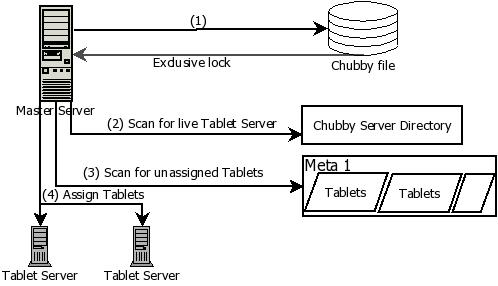
\includegraphics[width=5cm,   height=5cm]{. /figure/random. jpg}
	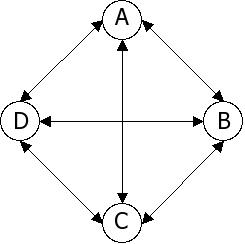
\includegraphics[width=.3\textwidth]{./figure/Solutions/Cassandra-cluster.png}
	\caption{A cluster of nodes in Cassandra}\label{f:cluster}
\end{figure}

Distributed system are prone to conflicts as many users could be issuing
requests on data items from any of the nodes. Any distributed system should
carefully consider conflict resolution and adopt design approaches which would
resolve such conflicts efficiently. Conflicts arise either at read or write operations.
The design approach should either make the system resolve such conflicts either
during one of these operations, deciding the system be either readable at all
times or writable. Cassandra optimises its performance by adopting the design
approach of resolving conflicts during read operations, making Cassandra always
writable.

All nodes in a Cassandra cluster applies the same architectural features
fundamental to Cassandra like bootstrapping, load balancing, replicating and partitioning data,
failure detection mechanisms etc. Some of the key architectural concepts are
explained in the following sub-section.



\subsection{Architecture} \label{ss:Cassandra-architecture}

Cassandra adopts a lot of its architectural concepts from other popular
distributed key-value data storage systems on the cloud, like Google's Bigtable
and Amazon's Dynamo. Overtime these adopted concepts evolved and developed new
features , some of which became specific to Cassandra's architecture. These
architectural concepts gave Cassandra its popular features like elastic
scalability, fault tolerance, high availability and high performance Cassandra's
architecture involves many sophisticated and complex theoretical as well as
mathematical concepts, some of which are discussed below. Discussing every
concept is beyond the scope of this research.

% The nodes in a cluster communicate with each other using the P2P communication
% protocol, Gossip. This protocol involves many complex mathematical models and
% help in significantly reducing the time taken to propagate requests from node to
% node (Raja, 2010).This protocol broadcasts any membership changes to all the
% nodes and allows nodes to reconcile such changes with its peer nodes.
% Using Gossip, nodes thus update their routing information about other nodes
% periodically. This also allows nodes to perform load balancing operations, i.e.,
% some workload is given to other nodes, when a node fails or has a high workload.



\begin{description}
\item[Peer-Peer Distribution Model:] Within a Cassandra cluster, all the nodes
are considered equal or identical in sharing responsibilities and
performing operations, in other words, all nodes are configured as peers and no
single node is a master or slave.  This is unlike traditional\acp{DBMS} that
are distributed, where nodes are configured such that they have different
responsibilities and roles. For example, some or one of the nodes is a master
and others are slaves.
Such a centralised configuration improves reading data, as data can be read from
any of the slave nodes, but write requests are always sent to the master node. This model
thus puts a lot of additional load on the master and also is prone to failure if
the single master node is offline. 

The peer-peer model in Cassandra is decentralized and  provides high data
availability since failure of some of the nodes does not affect the service of
the cluster, as other nodes can carry out the same operation or role. Similarly
this model makes new node additions to the cluster easy. Since nodes are
similar, no specific role has to be assigned to the new nodes, they just have to
be added to the cluster. Addition of nodes invokes the bootstrapping process,
which is explained later.

In a Cassandra cluster nodes use the peer-peer communication protocol called
Gossip for relaying information within the ring. Nodes sent state information at
regular time intervals using the gossiper so that other nodes in the ring can
know their status.

This is essential for failure detection in Cassandra. A gossip session is
initiated with a random node within the cluster during regular intervals where the initiator node  sends a
\texttt{sync} message to another node. If  the recipient node is active it would
return an \texttt{ack} message to the gossiper or the initiator. The initiator
then sends a second \texttt{ack} message to acknowledge the transmission and the
gossip session is completed. If the recipient node does not send an \texttt{ack}
message it is marked as dead and this information is logged.

When a node is found to be offline, after a gossip session, Cassandra implements
the \textit{hinted handoff} feature, to ensure that the operations that were
sent to the failed node are not lost (Figure~\ref{f:hinted handoff}). If a write request
was sent to the failed node, the node that now receives it would create a small
hint message with the information about the write request. This recipient node would use gossip
sessions to check the status of the failed node so that it can give the hint to
the failed node once it is alive again. A hinted handoff acknowledgement is
considered a successful write operation if the consistency level set by the
user, discussed under Eventual Consistency, is low., otherwise it is not
considered as successful and these hinted writes will not be readable. The hinted
handoff feature can be disabled in Cassandra if needed, depending on the suitability of the application using Cassandra.
\begin{figure}[h] 
	\centering
	%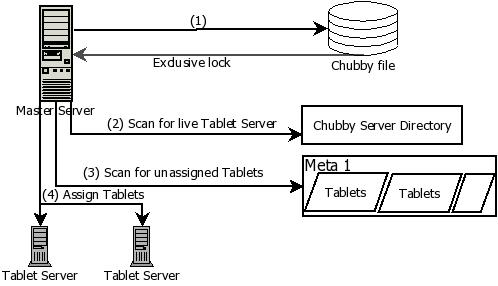
\includegraphics[width=5cm,   height=5cm]{. /figure/random. jpg}
	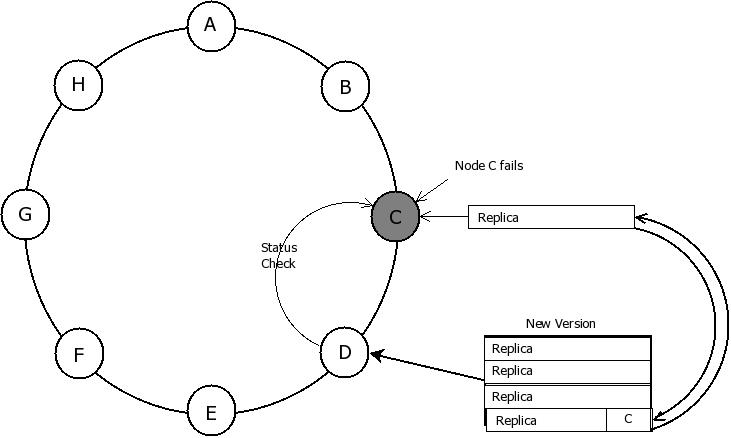
\includegraphics[width=.6\textwidth]{./figure/Solutions/Hinted-handoff.png}
	\caption{Hinted handoff in Cassandra}\label{f:hinted handoff}
\end{figure}

\item[Bootstrapping:] When a node starts for the first time, it checks its
configuration files to retrieve the location information of some of the
initial contact nodes or seed nodes.  It then chooses a random token, which is a
random value, for its position in the cluster and this token information of the
new node is gossiped to the other nodes in the cluster. This enables nodes to
have the routing information of all the peers in a cluster to send requests.
This is illustrated in Figure~\ref{f:bootstrap}, where \texttt{H} is a new node
joining the cluster after checking its configuration files and getting a token to join
the cluster. Its state information is then gossiped through the cluster. Node
\texttt{F} splits its ranges and send it to \texttt{H}, making \texttt{H}
responsible for the keys of that range.

\newpage

\begin{figure}[H]
	\centering
	%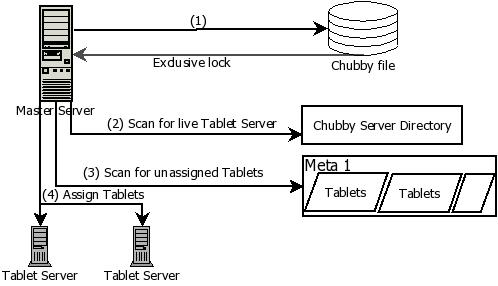
\includegraphics[width=5cm,   height=5cm]{. /figure/random. jpg}
	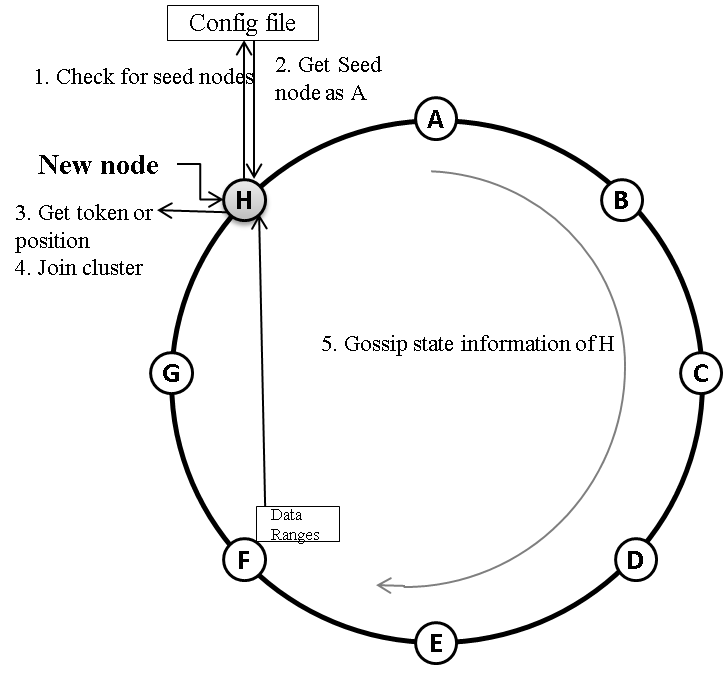
\includegraphics[width=.6\textwidth]{./figure/Solutions/Bootstrapping.png}
	\caption{Bootstrapping in Cassandra}\label{f:bootstrap}
\end{figure}

The token assigned to a new node would help balance the load of an overloaded
node, as some of the operations are transferred to the new node after all nodes
in the cluster know of its existence.  The new node thus is assigned a range
which belonged to another node. The bootstrapping algorithm renders Cassandra
the architectural feature of elastic scalability where adding new nodes is
simple and does not affect other nodes or operations in the cluster. This also helps in load balancing and ensuring that
the cluster has no bottlenecks of overloaded nodes clogging the cluster. To achieve
elastic scalability data has to be dynamically partitioned between the nodes,
which is explained next.

\item[Partitioning Data:] For  elastic scalability and efficient load balancing
Cassandra adopts the consistent hashing used by Amazon's Dynamo to partition
data over the nodes.(\todo{DeCandia et al.(2007)}). In consistent hashing, after
a node is assigned a place in a cluster, data objects that are identifiable by
their keys, are assigned to the node. Each data object's key is hashed and the
data object is sent
to the node that is larger than this hashed value (Figure~\ref{f:consistent
hashing}). This node is called the coordinator node for those keys stored on it.

\begin{figure}[h]
	\centering
	%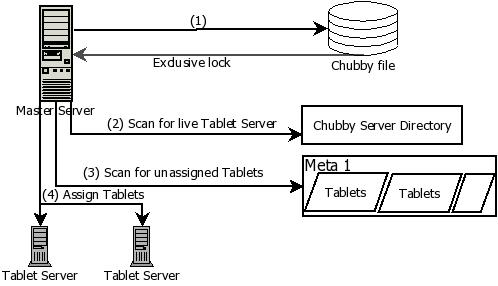
\includegraphics[width=5cm,   height=5cm]{. /figure/random. jpg}
	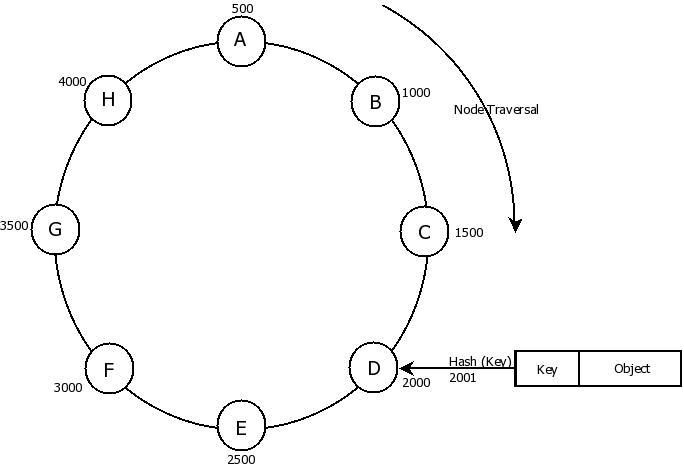
\includegraphics[width=.6\textwidth]{./figure/Solutions/Consistent-hashing-Cassandra.png}
	\caption{Consistent hashing in Cassandra}\label{f:consistent hashing}
\end{figure}

Partitioning data helps in load balancing as well as scalability of a cluster to
distribute workload to new nodes without affecting the performance of the
entire cluster. Additionally, in Cassandra better performing nodes are assigned
multiple points in the ring, making them virtual nodes and these nodes are assigned
  workloads from failed nodes or overloaded nodes. 

  \item  [Replication strategy]: For data to be always available to
  the users at all times, irrespective of failures, Cassandra uses a
  replication strategy. This involves replicating every object
  across several nodes by replicating a data item to N number of hosts, where N
  is the number of replicas that the user specifies. After consistent
  hashing, data items are assigned their coordinator nodes and these  nodes
  replicate the assigned objects (DeCandia et al., 2007). After saving the data
  items on locally, the coordinator nodes replicates the data items to N-1
  hosts. A preference list contains routing information about all the
  coordinator nodes that are responsible for storing a key (Figure~\ref{f:
  preference-list})which makes every node in the ring aware of which nodes are
  responsible for a key.
 
\begin{figure}[h]
	\centering
	%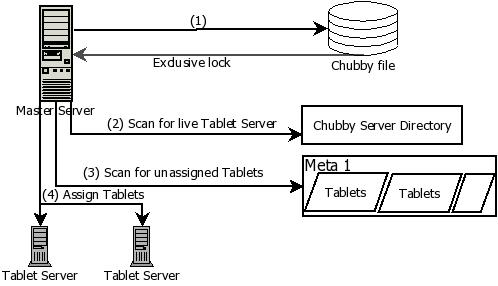
\includegraphics[width=5cm,   height=5cm]{. /figure/random. jpg}
	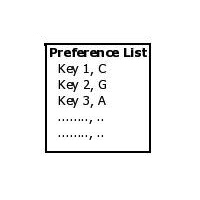
\includegraphics[width=.4\textwidth]{./figure/Solutions/Preference-list.png}
	\caption{A preference list example}\label{f: preference-list}
\end{figure}

Such a replication strategy makes Cassandra highly available as data items are
available from any node in the cluster and node failures do not
affect  data availability. All the nodes would know what ranges of key a
peer node is responsible for from the preference list and this helps in routing
requests to the correct nodes. 

Users can set the level of replication they would prefer, by setting the
replication factor to the number of nodes the users would like to use for
replication. In other words, replication factor tells the cluster how many
copies to save of a single data item. Setting the replication factor to a large
number would help in higher consistency of data items, but replicating data
items to a large number of nodes, each time there is an operation on it,  can
adversely affect the performance.

  \item [Eventual Consistency]:Consistency refers to the ideal scenario where
  all users read the same value of a data item, even when concurrent update
  operations are done on the data item.As mentioned previously, Cassandra opts
  for '\texttt{A}' and '\texttt{P}' of the CAP theorem and allows users to
  determine the level of consistency they would prefer by letting the users set
  the consistency level, which would tell the cluster how many
  replicas should acknowledge operations done on them, for the replicas to be
  considered consistent and up to date. Low consistency levels are considered
  better for performance as higher consistency levels involve more time
  since nodes have to wait to receive acknowledgements from more replicas.
  Letting the users decide the consistency level and replication factor means
  the amount of consistency is ascertained by the users. 

  To ensure the consistency between the nodes that the user sets in the
  consistency level, Cassandra uses the eventual consistency model, which is
  different from the commonly used strict consistency model in traditional
  \acp{DBMS} .
  Strict consistency models ensure that a read operation always returns the most
  update values. This is practical only in situations where the system using
  such a model is dependant on a single machine, where the operations are
  performed sequentially. But in distributed systems, where more machines are
  used, this leads to various conflicts when more than one user is involved. For
  distributed systems a weaker form of consistency, called eventual consistency
  is considered better (\todo{cite BOOK and marked papers}).
  
   Eventual consistency is where every replica agrees to the most recent value
   after a certain point in time and allows updates to be propagated to all the
   replicas asynchronously (Figure~\ref{f: eventual consistency}) (Henry, 2008). Thus, all replicas
   would be consistent eventually after a certain period of time, generally a small number of
   milliseconds \todo{cite book}.
   This requires that the replicas update the values in an order. Eventual
   consistency is useful when a distributed system has to scale greatly.
   If $N$ is the number of nodes containing replicas or the
  replication factor, $W$ is the number of replicas that should
  acknowledge a write operation and $R$ is the number of replicas
  that have to be contacted for a read operation (or the consistency level),
  then eventual consistency can be summarized as:%\\*
  
  \begin{equation}
  	W + R <= N \nonumber  
  \end{equation}
  
  This means that the consistency is not strict as the number of nodes to be
  contacted for a write or read operation is lesser than the number of nodes
  that hold the replicas.
  
  Cassandra performs \textit{read repairs} to make replicas of data consistent
  with the latest versions. Data inconsistencies are determined after checking
  the timestamps of the replicas by the node.  When during a read operation a
  node finds out that the replicas it received from a node  was not consistent with
  replicas on newer nodes, a read repair is performed on the node with the
  outdated replicas. This means that the older
  nodes are sent a write operation with the latest data. 
  
  \begin{figure}[H]
\centering
	% 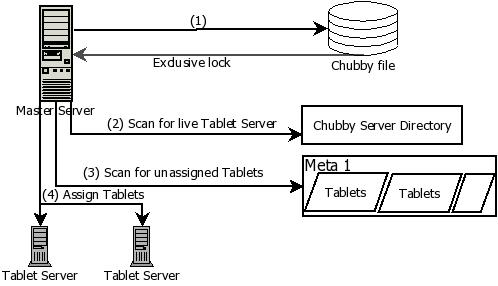
\includegraphics[width=5cm,   height=5cm]{. /figure/random. jpg}
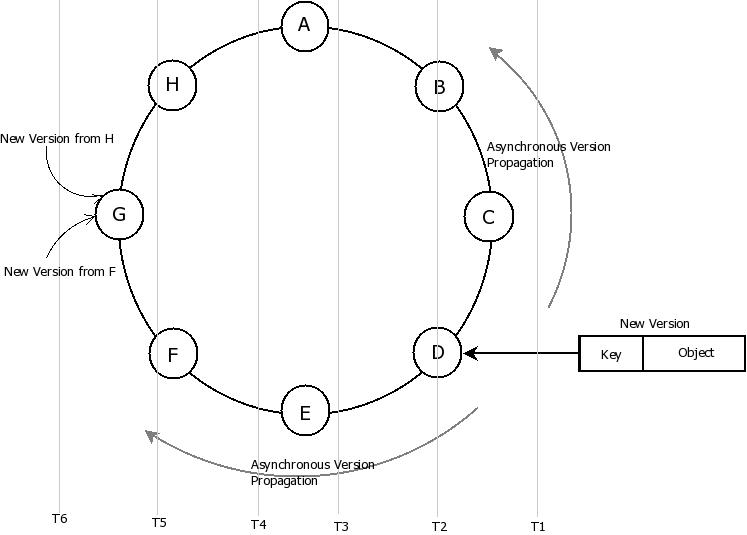
\includegraphics[width=.7\textwidth]{./figure/Solutions/Eventual-consistency-Cassandra.png}
	\caption{Eventual Consistency in Cassandra}\label{f: eventual consistency}
\end{figure}
   This time delay in updating all replicas could translate to latency in a
   large cluster of
  Cassandra nodes, where consistency level and replication factor is high. 
  
% 	  \begin{center}
% 	  \textbf{\texttt{\emph{W} + \emph{R}} \textless = \texttt{\emph{N}}}
% 	  \end{center}
  
  In Cassandra, users have two options while deciding the consistency level:
  single read and the quorum read. In a single read, the first data or replica
  that a node receives from another node is returned as a response to user's
  read request (Figure~\ref{f:singleread}). In a  quorum read, the node that
  receives a read request collects   replicas of data from majority of the available nodes in
  the cluster and returns the most updated data to the user (Figure~\ref{f:quorumread}).
  Quorum reads are slower when compared to single reads, but these prevent stale
  data to be returned.
  
    
  		 \begin{figure}[H]
			\centering
			% 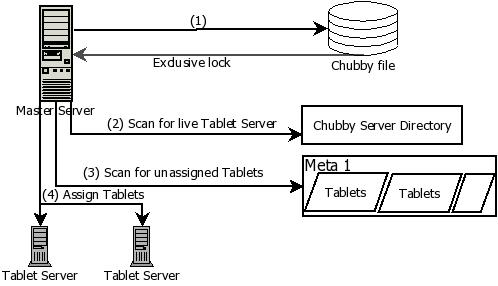
\includegraphics[width=5cm,   height=5cm]{. /figure/random. jpg}
			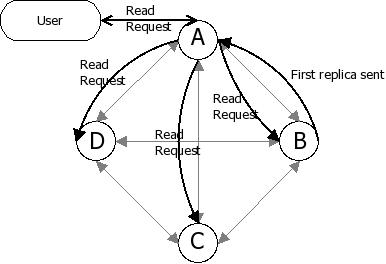
\includegraphics[width=.5\textwidth]{./figure/Solutions/Single-Read-Cassandra.png}
		
			\caption{Single Read in Cassandra}\label{f:singleread}
		\end{figure}
 
		 \begin{figure}[H]
			\centering
			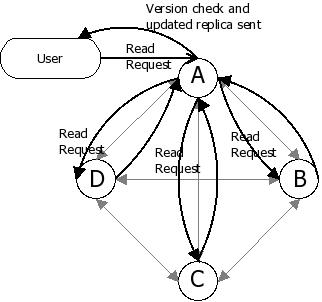
\includegraphics[width=.4\textwidth]{./figure/Solutions/Quorum-read-Cassandra.png}
		
			\caption{Quorum Read in Cassandra}\label{f:quorumread}
		\end{figure}


  
  \item [\ac{SEDA}:] \ac{SEDA} is a concurrency model designed for concurrent
  Internet services, which allows a single operation starting within a single
  thread to let the thread pass the operations to other threads. The work is
  divided into stages, where a stage comprises of an incoming queue, event
  handler and an associated thread pool. This thread pool decides which stages
  to be executed. This is unlike conventional applications where operations are
  run in a single thread. Such a concurrency model helps Cassandra enjoy great
  increase in performance as a stage can be
  controlled by different thread pools that also help in managing the available
  resources like disk space, network bandwidth for the stage to complete the
  work. Work that is divided into stages are mostly the operations like read,
  gossip, load balancing and the like.
  
\end{description}
\subsection{ Write and Read operations}
When users wish to write data into Cassandra tables, they send a write request
to a random node in the cluster (Figure~\ref{f:writeRead}). This node acts as the proxy
and writes the data to the whole cluster, thus efficiently replicating the data.
A user can set the number of nodes that should have the
replicated data copied on it and these replicas are saved on to nodes in the
same data centre and on other nodes in the other data centres. These nodes would act
as proxies when they receive requests from users (Perham, 2010a). This way even
if nodes fail, data is recoverable from other nodes.
		

Similarly, when a user makes a read request to a node, the node acts as a proxy
node and forwards the request to all the other nodes in the cluster
(Figure~\ref{f:singleread}).
As mentioned before, the level of consistency is specified by the user, i.e.,
single or quorum read. Nodes return data to the user after checking the versions
of the replicas and send the latest replica to the user and perform read repairs
on other nodes in the cluster (Perham, 2010b).
The technical details of how to read and write into Cassandra is discussed in
the following chapter.

\begin{figure}[H]
			\centering
			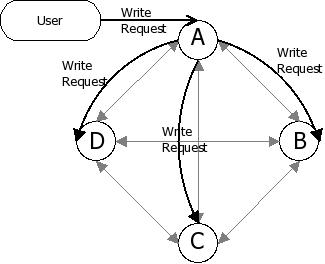
\includegraphics[width=.45\textwidth]{./figure/Solutions/Write-Request-Cassandra.png}
						\caption{A write and read operation in Cassandra}\label{f:writeRead}
		\end{figure}




% \acresetall
% %ब
\chapter{Proposed Solutions} \label{c:solutions}

% This chapter describes the four  solutions proposed to implement referential
% integrity constraints in a cloud \ac{NoSQL} database system.
% Section~\ref{} describes some typical ways of storing  data
% dependency information in \acp{DBMS}. Section~\ref{s:metadata} desribes how
% metadata is used for maintaining referential integrity in the proposed
% solutions. Section\ref{s:api} describes the design of the API devloped to
% implement these constraints.
Section~\ref{s:baseline} presents a baseline of
the \ac{API} without any referential integrity constraints
.


\section{Introduction}

As mentioned in the previous chapters, cloud \ac{NoSQL} database systems lack
referential integrity constraints that are imposed in traditional \acp{RDBMS} to
maintain data integrity. In \acp{DBMS}, data integrity is maintained by
correctly preserving the data dependencies existing between data entities within
a database.

Most popular traditional \acp{DBMS} do so by saving such dependency information
in their \texttt{SYSTEM} tables. This can be seen in porpular \acp{DBMS} like
Oracle, PostgreSQL, MS SQL Server etc. For example, in MS SQL Server 2000, there
exists \texttt{System} tables for every database that store various details of
constraints existing within the database. The \texttt{System} table
\texttt{sysforeignkeys} stores the information for all the foreign keys existing
in the tables in a database, like the objectIDs of the table with the constraint,
IDs of the referenced and referencing columns etc. This table is looked up
whenever referential integrity checks are triggered. \citep{sys:msdn}.
Similarly, in PostgreSQL, such information is saved as views which contain the
object dependency information for a database. The view
\texttt{table\_constraints} contains the information for all the constraints in
a table belonging to the current user.% \cite{}.
The information about the constraints within a database or a table that is
stored in such tables is the metadata information. Metadata is explained in
 Section~\ref{s:cloud-databases}

To understand how a cloud \ac{NoSQL} database system works and to deploy
the proposed solutions, the cloud \ac{NoSQL} database system Cassandra
is explored. The details of \texttt{Cassandra} is explained in
Section~\ref{s:cassandra}.

%


As mentioned before, these proposed solutions involve using metadata in
different ways to impose referential integrity constraints in Cassandra. The
following section describes metadata briefly. This


\section{Metadata}\label{s:metadata}
DBSs today tend to be large with respect to size or in terms of their
distribution across a network. Large-scale DBSs as well as large distributed
DBSs tend to also store and maintain metadata. Metadata generally is described
as ``Data about data''. Most of the literature talks about application
information, location information, directory hierarchy or access permissions as
the metadata that would be associated with the real data (Lin Xia et al. 2009;
Duval et al. 2002; Huang Bin \& Peng Yuxing 2010; Hackl et al. 2010; Jan-Jan Wu
et al. 2010). But in addressing the current problem of RI in NoSQL DBSs,
thepotential solutions consider storing information about dependencies or
relationships between the data entities as metadata. This metdata could then be
stored as a table(s).

In (Hackl et al. 2010) metedata management is discussed where emphasis is laid
on the synchornous updates of metadata storage. While this paper focuses on
metedata management, an interesting approach is adopted in a key-value DBS as a
part of their experiment. Metedata is managed in TokyoCabinet by inserting the
metadata in the value field, separated with semicolons (Hackl et al. 2010)

For creating metadata tables like the one shown above, it would be necessary to
derive the dependency information from the ER designs of the database. The
dependencies could then be inserted into the metadata tables using the
MetaDriver low-level API, which is described below.
 would be a reserved keyword or identifier to distinguish the
tables as metadata tables from other tables or ColumnFamilies. Since these
metadata tables could be stored on different server nodes as a part of the MDS
cluster, it might be necessary to give the metadata tables a unique name too.
For this purpose such metadata tables could have the names of their respective
databases prefixed to the '' keyword, like 'StudentMDCONSTRAINT'
as shown in Figure 6. For example, if the metadata table is designed for a
hospital DBS, it could be named as '', which would help
the MetaDriver API identify it as the metadata table belonging to the Hospital
DBS. Such a unique identifier is needed due to the distributed nature of the MDS
cluster. (Please note: The protocols needed for such an MDS cluster would be
discussed in following reports.) When an application using a NoSQL database
interacts with the database to perform any operation on the data like inserting
or updating or deleting data etc., the application normally talks to the
database engine or database driver. In NoSQL databases, this is commonly done by
the APIs the NoSQL DBMS provides, for example Thrift in Cassandra, JDO in Google
AppEngine etc. The proposed solution is an API, called MetaDriver, would be a
layer on top of such APIs. This is shown in Figure 7.

In the proposed solution, the value could include metadata about what table or
what foreign value the value of a key-value pair would refer to. Here, the
foregn value is similar to the foreign keys in RDBMSs, except that the foreign
value is not the unique primary key

In the case of NoSQL DBSs, this could mean that every replicated copy holds the
same metedata information in the value field. So values that refer to other
values in different tables could be maintained.

\section{The API and Database Schema/Model}\label{s:api}

To perform data operations like insert, update, delete, retrieve data
etc.,Cassandra provides an \acp{API} to its users. The Thrift API can support
many programming languages, making it easy for most applications to store data in
Cassandra (Gunda, 2010). For the proposed solutions, Hector, an \acp{API}
designed to work above the Thrift \acp{API} is implemented.--(\todo{Hector
details})-- This helped develop the solutions faster due to its simplicity and
efficiency in communication with Thrift \ac{API}.

The proposed solutions are writted in Java and run on a cluster
of nodes within the university's computer network. During the development a
cluster of 5 nodes were used and for testing this was increased to
(\todo{node\#}).

Pseudocodes give an informal and a high-level description of an algorithm
without using variable declarations, function calls or complicated data flows
and replaces these with simple English sentences (Wikipedia 2011). Since the
current purpose is simply to understand the key principles and steps involved in
the proposed solution, pseudocodes are the best way to describe all this without
using any conventional programming syntax. For the sake of simplicity, in the
following pseudocodes any kind of database operation is termed as request and
the metadata table is assumed to be similar to 'StudentMDCONSTRAINT' in Figure
6

The API inserts data into the column families from CSV files. The Students and
Courses details are inserted without performing any insertion checks. On the
other hand, the Enrolment column family would have referenced columns from other
column families. So it was required that checks be made prior to insertion, to
ensure that the referenced values were actually existing in the referenced
column families. For example, when the following row is to be inserted into
Enrolment some checks would have to be made to ensure data consistency and
integrity

Generally, the referential integrity constraint needs to hold whenever any data
operation is performed on the data. Referential Integrity (RI) checks are
performed each time an update operation is invoked on any entity like Student or
Course or Enrolment. As previously mentioned, the dependency information for all
entities is saved as metadata and for each solution this metadata is saved in a
different way. But for all the solutions, the RI checks for an update operation
are similar.
In an update operation there are two different types of RI checks performed,
depending on the entity that is being updated. Update RI checks for a parent
entity are different from the update RI checks for a child entity. Also, the
update operations are different depending on the 'DeleteRule'.
A parent entity contains the key that is referenced by another entity, i.e.,
child entity. Therefore, the child entity is the one with the referencing key or
the foreign key. For example, the entities Student and Course are parent
entities, while Enrolment is a child entity.Whether data is being inserted,
updated or deleted, referential integrity has to be adhered to. The actions and
the checks to be performed for each of such operations are described below.

\subsection{Insert}
  %An insert operation would trigger a referential integrity
%   validation when data is being inserted into a referencing table, i.e., the child table. In
% such an event, prior to entering the values in the referencing table, it is
% checked if the referencing keys exist in the referenced table. For example, when
% the enrolment details of a student are being inserted into the Enrolment table,
% a check is triggered to verify whether the StudentID exists in the Student
% table. Similarly, it is also verified that the CourseID exists in the Course
% table. If the referencing keys do not exist in the referenced tables, then the
% insert operation is not allowed.
Prior to inserting this row, insertion checks would be made to ensure
that the SID exists in the Student Column family of the keyspace University. This piece
of information can be retrieved from the second part of the metadata
information. This is applicable to all solutions, as metadata information is
consistent across all solutions. Similarly, the Course column family would have
to be checked to ensure that SWEN100 exists. If these checks are not
implemented, then it is possible that any wrong information can be inserted and
the referential integrity constraint be violated. For example, SWEN100 may not
actually exist in Course, but without any checks it could be inserted into the
database.

Such insertion checks are introduced into all the solutions within the API.

 \subsection{Update}
 %When data is being updated either in the referencing
 % table or
% the referenced table, a referential integrity validation is needed. When any
% referenced key (primary or unique) is being updated in the referenced table,
% then it has to be verified whether this key is a foreign key in any of the
% referencing tables. If a dependency is found to exist, then the applicable
% referential integrity rule is checked. So if it is a Cascade, then the
% associated foreign keys in the referencing table are updated prior to updating
% the key in the referenced table. If the rule is "Set to NULL" or "Set to
% default" then the associated foreign keys in the referencing table are set to
% NULL or default values. A Restrict would prevent the update action in the
% referenced table.
%
% When any foreign key is being updated in a referencing table, then a referential
% integrity validation has to be performed. It has to be ensured that the new
% updated value exists as a key in the referenced table. For example, in the
% Enrolment table, if the course details of a student (i.e. foreign key CourseID)
% are being updated to a new value, then it has to be verified that the new value
% is an existing key in the Course table. Otherwise, if the new value does not
% exist, then the update is not allowed generally.

When an update is made to a value in a column family, checks have to
be made ensuring that these changes or updates do not violate referential
integrity. Update actions would overwrite data and if such actions overwrite
values that have dependencies on them, it could lead to poor integrity. The API
would first check if the value that is being updated exists in the metadata
information as a Primary key or as a foreign key. If it is a part of the
metadata information, implying that a constraint exists on this value, then the
update would be prevented from execution and an exception would be raised.
A different kind of Update is the Upsert, where the values would be inserted if
the values to be updated do not exist already. Here, the API would check if
there are any foreign keys being inserted and would check to see if they exist
in the mentioned keyspace prior to executing the Upsert operation.
\begin{description}
\item [Updating a parent entity:] When a parent entity is being updated, its
metadata information is checked to find out its 'DeleteRule'. 'DeleteRule' for an entity
could be 'NODELETE' or 'CASCADE' and is applicable for both delete and update
operations. If the 'DeleteRule' is 'NODELETE', then the update of the entity is
not allowed. For example, in the current API, Course entities have a 'NODELETE'
rule in their metadata while the Student entities have a 'CASCADE' rule. Hence,
when a request is made to update a Course, it is not allowed by the API and an
exception is thrown. Despite this, a further check is made to see if the entity
has any child dependencies existing or not. In this dependency check, if the
entity is found to have no dependencies, the update is allowed.  For example, if
a Course entity is found to have no students enrolled for it in Enrolment, the
update operation is allowed and the Course is updated with the new value.

If the 'DeleteRule' is 'CASCADE', then the metadata is checked to identify the
referencing column families. The existence of the record marked for update in
these referencing column families is verified. If existing, the child records
are updated with the new value. Then the values in the parent entity are updated
with the new value. For example, if an update operation is invoked in the
Student column family, to change 'StudentID' '111' to '222', and its
'DeleteRule' is 'CASCADE', then the referencing column family, Enrolment is
identified using the metadata. In Enrolment, all the existing values for the
foreign key '111' are replaced with '222'. Then the 'StudentID' in Student
column family is updated to the new value '222'. Hence, the child records are
updated prior to updating the parent record in the referenced column families.

\item [Updating a child entity:] When a child entity is updated, it is first
verified whether the new update value exists in the referenced parent entity. If it
exists, the foreign keys in the child entities are updated with the new value;
else an exception is thrown as the new value does not exist in the parent
entity. For example, in the child entity Enrolment, if an update operation to
change the 'CourseID' 'SWEN100' to 'COMP100' of 'StudentID' '111' is issued,
then it is first checked if the new value 'COMP100' exists in Course column
family. The Course column family is identified as the parent or referenced
column family by looking up the metadata information for Enrolment. If 'COMP100'
is found to exist as a key in Course, then the foreign keys in Enrolment are
updated with this new value else an exception is raised and the update operation
is aborted.
Similar to the delete operation, the update RI check is performed by the
ValidationHandler method in the application (Figure 1). If no dependencies are
found, the entity is updated. Unlike the delete operation, for update the
ValidationHandler checks for the 'ConstraintType' 'F' which indicates a foreign
key in the child entity.
\end {description}
Hence Update operation updates the column families with the new values only if
the referential integrity is maintained consistently across both the referenced
and referencing column families.


 \subsection{Delete} %A delete operation would trigger a referential
 % integrity
% validation when data is being deleted from the referenced table. When data that is marked
% for deletion is found to have dependencies in other referencing tables, the
% referential integrity rule applicable for this operation has to be checked. If
% the rule allows Cascade, then the depending values in the referencing table have
% to be removed prior to deleting values from the referenced tables. If it is a
% "Set to default" or "Set to NULL" rule, then the referencing foreign keys would
% be set to NULL or default values in the referencing table. A Restrict would
% prevent data from being deleted if it is found to have dependencies in other
% tables. For example, while deleting a student record form the Student table, a
% check is performed to see if the StudentID is a foreign key in any other table.
% In this example, the Enrolment table would be checked and when the StudentID is
% found as a foreign key, the appropriate action is performed depending on the
% rule. If it is Cascade, the enrolment details of the StudentID are removed from
% the Enrolment table and then the Student record is deleted from the Student
% table.

Referential Integrity (RI) checks are performed each time a delete
operation is invoked on any entity like Student or Course or Enrolment. While
saving these entities, their dependency information is also saved as metadata.
For each solution, this metadata information is saved in a different way. For
example, in Solution 1, metadata is saved as a part of the value separated by
special characters, in Solution 2 it is saved as a top row, in Solution 3 it is
saved as a separate column family and in the final solution it is saved on a
cluster of nodes dedicated for saving metadata column families. Despite the
different ways of saving metadata, the delete checks for RI are mostly
consistent across the solutions.
When an entity is being deleted, its metadata information is checked to find out
the DeleteRule of the entity. DeleteRule for an entity could be NODELETE or
CASCADE. If the DeleteRule is NODELETE, then the deletion of the entity is not
allowed. For example, in the current API, Course entities have a NODELETE rule
in their metadata while the Student entities have a CASCADE rule. Hence, when a
request is made to delete a Course, it is not allowed by the API and an
exception is thrown. But despite this rule, a further check is made to see if
the entity has any dependencies existing or not. In this dependency check, if
the entity is found to have no dependencies on it, a delete is then allowed.
For example, if a Course entity is found to have no students enrolled for it in
the Enrolment column family, the delete operation is allowed and the Course is
deleted.
This check is performed by the ValidationHandler method in the application as
seen in Figure 1 . The ValidationHandler is invoked whenever a Delete, Update or
an Insert operation is invoked on any entity. The ValidationHandler checks for
any dependencies for the entity even when the DeleteRule  is NODELETE . If no
dependencies are found, the entity is deleted.

Figure 1: Pseudocode for RI checks for NODELETE Previously, upon finding a
NODELETE rule, any further checks for dependencies were not performed and the
entity was strictly not allowed to be deleted. As a result, a Course entity that
had no students enrolled was prevented from being deleted.
By making the delete rule less rigid by accommodating deletes of entities with
no dependencies, it allows the API to maintain proper data integrity and adhere
to RI rules.



\section{Baseline:  }\label{s:baseline}


\section{Solution 1:  Metadata with Special Characters}\label{s:sol1}

In RDBMSs, referential integrity constraints are enforced at the creation of
tables (or updated later using ALTER TABLE). In the above example, imposing the
referential integrity constraint for the Enrolment table (Figure 3) would be
using "FOREIGN KEY CourseID REFERENCES Course (CourseID)". This would indicate
that the CourseID of Enrolment table is dependant on the CourseID primary key of
the Course table.
The first proposed solution involves saving the dependency information as a part
of the value separated by a semicolon. Trying to achieve this in Bigtable means
that the supercolumnfamily of 'Enrolment' would need to save the dependency
information as a part of the value itself for every key-value pair. In this
example, this would mean saving the dependency information as
";SuperColumnFamily (Course:CourseID) REFERENCES ColumnFamily
Course(CourseID)".This is illustrated in Figure 6. This would mean that the
CourseID values of all Course SuperColumns are dependant on the key-value pair
of CourseID (Figure 7) which belongs to the ColumnFamily of Course.

In (Hackl et al. 2010) metadata management in distributed environments is
discussed where emphasis is laid on the synchornous updates of metadata storage.
While this paper focuses on metadata management, an interesting approach is
adopted in a key-value DBS as a part of their experiment. Metadata is managed in
TokyoCabinet, a NoSQL DBS, by inserting the metadata in the value field,
separated by a special character like a semicolon (Hackl et al. 2010).To
illustrate this solution, as well as the rest of the proposed solutions, in this
report an example of university department keyspace would be used. This keyspace
would have a Student column family, a Course column family and an Enrolment
column family that contains data about all the students and the courses that
they are enrolled in. In such a keyspace, the metadata for the value field of
the Student is shown below.

A student could be enrolled in a number of courses and if any student is
enrolled into a course that is not in the course column family it would be a
dangling reference or violation of referential integrity. This would lead to
inconsistent and invalid data and would lead to poor data integrity.
In the case of NoSQL DBSs, this could mean that every replicated copy holds the
same metadata information in the value field. So values that refer to other
values in different tables could be maintained.

In the revised Solution 1, this metadata information was made more precise and
detailed. It now would hold the information about the keyspace the constraints
belong to, the field that is the Primary key and also gives information about
where it would have dependencies in. So a Student column family would now look
like

This metadata information starts and ends with special characters, the curly
brackets. The metadata information is separated by semi-colons. The first part
of this metadata information, "University,P,Students,University,,SID", gives the
following information:
\begin{itemize}
\item Keyspace:this constraint belongs to: University
\item Type of constraint:Unique Key or Primary Key denoted by 'P'
\item Column Family: The Column family this constraint belongs to: Students
\item Keyspace: The keyspace this column family exists in: University
\item Referenced Column Family: If this was a Referential Intergrity another
value indicating the foreign column family is provided. But here, because it is a Primary key constraint, it
is left blank.
\item Unique Key: The column which is the unique key: SID
\end{itemize}

Therefore, this first part of the
metadata provides information about the primary key for the column family.
The second part of the metadata information,separated by the semi-colon,
University,R,Enrolment,University,SID,cascade, gives the following information:

\begin {itemize}
\item Keyspace:this constraint belongs to: University
\item Type of constraint:Referential Integrity constraint denoted by 'R'
\item The foreign Column family this
constraint would be a foreign key in: Enrolment
\item The keyspace this column family exists in: University
\item The column that would be the referenced key in the foreign Column family:
SID
\item The type of delete rule that would be applied on this constraint:
cascade
\end{itemize}
This second part of the metadata provides the details of any of the columns in a
column family that is a foreign key elsewhere.

These changes to the metadata information involved more parsing of the metadata
information in the API, but on the other hand it provided consistency across all
the solutions, by keeping the format of the metadata information consistent
throughout the solutions. The metadata also provided more information about the
constraints and were clearer.


\section{Solution 2:  Metadata as Top Row}\label{s:sol2}
Similar to solution 1, solution 2 proposes to have the metadata information
saved within the column family. Instead of separating it using special
characters, this solution proposes to include the metadata as a top row in every
column family. This is illustrated below:

Like solution 1, every replicated copy of the column family carries the metadata
along with it on ever node.
The proposed API for implementing these solutions would check the top row prior
to any delete operation. So if a course is being deleted, the top row of Course
column family would be checked to see if any other column family depends on it
or not. Then the appropriate action is performed.


\section{Solution 3:  Metadata Tables}\label{s:sol3}
The metadata table would be modelled around the 'System' tables in Oracle or
other popular DBMSs, where all the constraint information is stored. The
metadata table in this solution would record and save the constraint information
of all the column families in a keyspace. Here, the metadata table would show
all the existing dependencies in a column family and would belong to the same
keyspace as the column families.
Even if a keyspace has multiple column families, all information about the
dependencies of various values in the column families would be stored in this
metadata table.
This metadata table would be queried whenever any delete operation is issued.
Here, if any Student value is being deleted it would be checked if the Student
Primary Key (SID) values exists in any of the 'RColumn' column of the metadata
table. If it does exist, then the action to be performed is determined from the
'DeleteRule' column.

\section{Solution 4:  Metadata Clusters}\label{s:sol4}
But simply providing thereferenced table/value, as seen in figure does not
ensure the correctness or consistency of thedependency. Though this solution
appeals in simplicity it has its own restrictions. Each time a value is
accessed, whether for updating the value or deleting it, a check has to be
performed for any dependant values. When a foreign value is updated or deleted
every value, in a key-value pair, depending ont his foreign value would have to
be idetified and correctly updated. This is due to the decentralised way in
which the metadata is spread in this proposed solution. All the tables would have to
be queried and the values that would be affected by this change in foreign value
would have to be individually updated.  Having to access access every record to
check its metadata and then to change it would turn costly if the database is a
large one,i.e., either in terms of large scale data or in terms of the way the
database is spread/replicated on several nodes or both large scale data and wide
distribution and rpelication. This would be very time consuming, especially
since data on the cloud does not have geographic boundaries either.
Instead, having metedata separately stored decoupled from real data would be
preferrable. This would mean that every record or key-value pair need not be
accessed to learn about their metadata. This is seen generally in most
distributed systems today, where metadata server clusters are deployed to store
metadata (Lin Xia et al. 2009). Metadata server is a software that helps in
performing administrative and management services of metadata (IBM Corporation
2003). These metedata servers are often clusters in large distributed
environments for better scalability and efficient access/availability of
metadata. Such a cluster could have a master metadata server and subordinate
meteedata servers, with each server running on a different node.These servers
also provide clients who access the meetdata with locking facilities, policies
etc. too(IBM Corporation 2003). An illustration of such a metedata cluster,
where metedata is stored on different nodes is given in

Some researchers (Huang Bin \& Peng Yuxing 2010) also claim that DaaS is
beginning to adopt this architecture of separating the metadata from the real
data. MDS clusters can be used as a solution to resolve the current problem of
enforcing RI in NoSQL DBSs. Metadata in this solution would be held in tables
that hold the dependency information of the values in any key-value pair in
NoSQL  DBSs.  An example of a metadata table is shown in

Generally, in most distributed systems today, MDS clusters are deployed to store
metadata (Lin Xia et al. 2009). MDS is a software that helps in performing
administrative and management services of metadata (IBM Corporation 2003). For
better scalability and efficient access/availability of metadata, MDS are often
separate clusters in large distributed environments. Such a cluster could have
a master MDS and subordinate MDSs, with each server running on a different node.
MDS clusters can be used as a solution to resolve the current problem of
enforcing referential integrity in NoSQL DBSs too. Similar to Solution 3,
metadata in this solution would be held in separate column families. But instead
of saving the metadata tables as a column family of the keyspace, the metadata
table would be saved in a separate cluster. The API would then talk to the MDS
cluster as well as the Cassandra cluster before every delete operation.
This would mean that the metadata storage is decentralised again and separate
from the database cluster. It is assumed that this would lead to better
performance as the MDS would not be as widely replicated as the Cassandra
cluster and incurs less computational costs.


This metedata table would show all the existing dependencies in a database.
Evene if a database has multiple tables, all information about the dependencies
of various values in the tables would be stored in this metedata table. Each
entry in this metedata table could have a unique key. This is explained later.

\section{Analysis of results}\label{s:summary}

\begin{figure}
	\centering
	%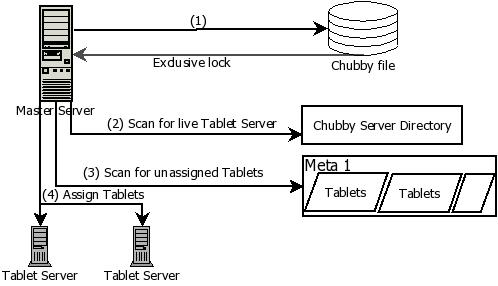
\includegraphics[width=5cm, height=5cm]{./figure/random.jpg}
	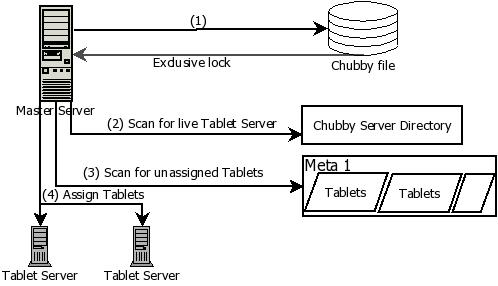
\includegraphics[width=.5\textwidth]{./figure/random.jpg}
	\caption{Random Pic}\label{f:random-pic}
\end{figure}


\begin{figure}

\begin{verbatim}
{
    "firstName": "John"
    "lastName" : "Smith",
    "age" : 25
}
\end{verbatim}
\caption{JSON}
\end{figure}


%
\acresetall
%ब 
\chapter{Results and Discussions}
% The results and discussion for each solution considers the time taken for
% operations to complete on each of the entities  as described in the University
% example adopted for the experiments.

% Performance of database systems is commonly measured in terms of the
% \textit{Response time} and \textit{Throughput}(\todo{cite Demurjian, Berkely}).
% Response time refers to the time  a database system takes to process an
% operation and produce results to the end user . Measuring response time for a
% database operation is similar to a black-box evaluation because it is measured 
% without considering the internal functioning  of the database system. According
% to (\todo{cite Demurjian}) such an evaluation is ideal for a complete database
% system to measure its performance and to give the users details about its 
% efficiency and speed in performing operations. In this thesis, response time and
% throughput are the measures used to gauge the performance of Cassandra
% while referential integrity validation is implemented using the \ac{API}.
% 
% Response time for each of the  operations that trigger such a validation from
% all the solutions are measured during the experiments. This included the
% time involved to access and retrieve metadata for the entities and also the time for
% validating referential integrity by the \texttt{ValidationHandler}. The response
% time of Cassandra when such validations are not in place is also measured and considered as a
% baseline with which to analyse the solutions. Such a comparison  determines the degree of
% change in speed of Cassandra when such overheads are introduced and gives 
% users useful information about how each solution affects the performance of
% the database system.
% 
% The second performance measure used is \textit{Throughput} which
% is another classical and commonly used measure of database performance
% (\todo{cite BerkleyDB}).
% Throughput measures the number of operations processed by the database system in a unit of
% time. In the experiments the throughput for all the operations
% triggering referential integrity validation across all solutions is measured
% as operations per second.
% A single operation stands for each time an entity is inserted or updated or
% deleted. 
% % For example, inserting 1000 students means that 1000 \texttt{insert}
% % operations are processed by Cassandra. 
% Note that only the operations that
% introduce the referential integrity validation in Cassandra is measured and thus
% \texttt{read} operations are not measured in terms of response time or
% throughput.
% % These operations
% % which trigger referential
% % integrity validation for an entity
% % namely the \texttt{insert}, \texttt{update}, \texttt{delete} operations are
% % were measured in terms of the throughput in the experiments. Throughout commonly
% % referes to the number of operations performed
% 
% It has to be noted that the operations are prone to  external factors like
% network latency, bandwidth, network routing, network workload among others which
% typically affect a network consisting of several machines and users. This is
% because the Cassandra cluster used in the experiments is deployed over a
% network that is used by many users concurrently thus exposing the operations to
% such factors. Identifying such factors and analysing them is beyond the scope of
% this thesis and the analysis is strictly in terms of how the metadata storage
% and referential integrity validation affects Cassandra's performance.

 The results from the experiments were used to
analyse the performance of the four solutions with respect to  response
time and throughput and this is discussed in the following sections.
Section~\ref{sr:baseline} presents the results for the baseline experiment where 
% no referential validation checks are implemented
% and t
the operations performed on the entities are just as it would be performed in
Cassandra. Section~\ref{sr:insert} analyses the results of all the solutions
for the \texttt{insert} operation. Section~\ref{sr:update} presents the analysis
for the \texttt{update} operation for all the solutions. Section~\ref{sr:delete}
discusses the results of the solutions for the \texttt{delete} operation. 


\section{Baseline}\label{sr:baseline}
The performance of Cassandra when referential
integrity validation is introduced using any of the solutions is compared with a
a base experiment where the operations on the entities do not trigger any
such validations. Such a baseline is useful to determine the
performance of the database system when validations are imposed using the
\ac{API} and to analyse the performance of the solutions.
% baseline experiment has no referential integrity validation introduced and
In the baseline experiment, the operations on the entities represent how
data is inserted into Cassandra without referential integrity validations. The
results in terms of response time for the baseline experiment is presented as
a bar-plot in Figure~\ref{fr:Solution0-barplot}. The analysis of
the performance of each operation on an entity is discussed as follows.
% The results are analysed in the
% following 

% The factors measured were the time involved to complete each operation for every
% entity, where the operations considered were the ones that invoked referential
% integrity validation, namely, \texttt{insert}, \texttt{update} and
% \texttt{delete}. These were measured for the entities in the University example,
% namely \texttt{Student}, \texttt{Course} and \texttt{Enrolment}.
% The results are plotted as a histogram in Figure~\ref{}
	
\begin{figure}[h] \centering
\includegraphics[width=.8\textwidth]{./figure/result/Solution0-barplot.png}
		\caption{Baseline}\label{fr:Solution0-barplot}
	\end{figure}
	
% Present results.
% 	The potential reasons for the variance of time for the completion of each
% 	operations on the different entities are summarised next.
	\begin{description}
	\item[Insert] The results from the baseline experiment show that the time for
	inserting entities into the \texttt{Student} and \texttt{Course} column families 
	are similar. This is because the number of entities inserted into these
	column families are exactly the same.
% 	\texttt{1000} instances of \texttt{Student} and \texttt{Course} are inserted
% 	into the respective column families in the baseline experiment. 
	The time taken
	to insert the \texttt{Enrolment} entities into the \texttt{Enrolment} column family
	is higher by approximately \texttt{4} seconds. This is because
	\texttt{Enrolment} has more entities than the other column families, to be
	specific it has \texttt{10,000} instances which is 10 times more entities than
	\texttt{Student} and \texttt{Course}.
% 	Hence, the \texttt{insert} operation takes more time to insert entities into \texttt{Enrolment} column family, especially considering its
% 	replication across \texttt{10} nodes, which would add to the time in
% 	completing the operation.
	
	\item[Update] The time for updating the primary keys in \texttt{Student} and
	\texttt{Course} are comparable to each other. Although the number of entities
	updated are the same, the small difference is owing to external variables
	(e.g. network latency, high network traffic). Similar to the \texttt{insert}
	operation, updating the \texttt{Enrolment} entities takes significantly more
	time, which is again due to the higher number of entities held within this
	column family. 
	
	The  response time of the \texttt{update} operation on
	\texttt{Enrolment} is higher when compared to the response  time of
	\texttt{insert} operation on the same. This is mainly due to the additional
	computational resources consumed to ensure the existence of an entity before
	updating it to new values.
	
	\item[Delete] The time involved for completion of the \texttt{delete} operation
	on all the entities from \texttt{Student} and \texttt{Course} column families
	are similar to each other owing to the same number of entities. The time
	involved for the \texttt{delete} operation to delete all the entities in
	\texttt{Enrolment} is higher just as in other operations. This is again due to
	the larger number of entities present in \texttt{Enrolment}.
	
	Performance of the \texttt{delete} operation is similar to the\texttt{insert}
	operation in terms of time taken for completion and the processes involved. This
	means that unlike \texttt{update} both \texttt{delete} and \texttt{insert} do
	not involve additional operations and simply adds or removes entities from the
	column families. It should also be noted that external factors affect the
	performance of the operations.
	
	\end{description} 

	
	
% 	Explain Insert. Why student and course similar. Why enrolment much higher.
% 	

	In general, all the operations take more time to complete on the
	\texttt{Enrolment} column family due to its larger number of entities 
	when compared to \texttt{Student} and \texttt{Course} column families. The
	\texttt{update} operation consumes more time due to the additional search
	involved to locate the previous state of the entity prior to updating it to new
	values. Notice that the time involved to complete \texttt{insert} and
	\texttt{delete} entities form all the three column families are similar.
	
	The following sections analyse the performance of each solution  in
	terms of how its referential integrity validation in each of the
	\texttt{insert}, \texttt{update} and \texttt{delete} operation and its
	metadata storage affect the performance.
	
\section{Insert}\label{sr:insert}
An \texttt{insert} operation triggers a referential integrity validation
whenever a child entity containing foreign keys is inserted where the
\texttt{ValidationHandler} validates that the foreign keys exist as primary keys in the parent
entities. 
% This dependency information is retrieved from the metadata saved in
% each solutions. 
In the experiments, the time taken to insert all the
entities are recorded thus also measuring the time involved for validating
referential integrity for each entity. Across all the solutions in the
experiments, the \texttt{insert} operation triggers such a validation when the
\texttt{Enrolment} entities are inserted since it is a child entity containing
foreign keys of \texttt{Student} and \texttt{Course} entities.
%  As mentioned in
% Section~\ref{s:exp:setup} the number of entities inserted into the
% \texttt{Enrolment} column family is the same for all solutions and the baseline
% experiment.
% Despite the same number of entities and similar validation performed, 
The response time and throughout of the \texttt{insert} operation in all the
solutions and the baseline experiment are plotted in
Figure~\ref{fr:insert-result}.
% 	\begin{figure}[H] \centering
% 	\includegraphics[width=.8\textwidth]{./figure/result/op-insert-barplot.png}
% 		\caption{}\label{fr:response-insert}
% 	\end{figure}
	
	
	
	
	
	
	
	
The results of all the solutions as seen in Figure~\ref{fr:insert-result} with
respect to response time  is discussed as follows based on the different
entities on which the \texttt{insert} operation is applied.
\subsection{Response Time}
\begin{itemize}
  \item The results show that the response time of all
  the solutions to insert entities into \texttt{Student} and \texttt{Course}
  column families is similar and always lesser than 5 seconds. This is because
  no referential integrity validation is invoked when parent entities are
  inserted as these do not contain any foreign keys. Note that the metadata for
  any entity is accessed and checked by the \texttt{ValidationHandler}
  to determine if it has dependencies or not. It is during this
  check that it is determined if an entity is a parent or child. 
  So across all solutions even when parent entities \texttt{Student} and
  \texttt{Course} are inserted their metadata is accessed.
  
  Solutions~1, 2  and 4 have approximately similar response times since the metadata 
  access for these solutions are easier as metadata is a part of the entity and 
  no additional connection to a metadata column family is required. Solution~3
  takes slightly longer than the rest of the solutions and this is because of the way
  the metadata is accessed for the entities in this solution. 
% irrespective of whether an entity is a parent or child the
% \texttt{ValidationHandler} performs the same check the metedata of the entity
% for all the solutions. It is when this check is made it is clear if the entity
% is a parent or child. 
  In this solution accessing the metadata for every 
  \texttt{Student} and \texttt{Course} entity causes the slower
  response time since a different \texttt{Metadata} column family has to be
  accessed using the connection object. This is because metadata is not cached
  for re-use in this solution. Unlike this, Solution~4 caches  metadata for
  entities and re-uses it thus saving time by not having to access a separate
  column family for each entity insertion.
  
  When compared to the baseline experiment the insertion of parent entities
  in all the solutions, except Solution~3, take similar response times despite
  the initial metadata access. Solution~3 takes only a few seconds
  longer to complete the operation when compared to the baseline.
  


  \item The response time involved for inserting the \texttt{Enrolment}
  entities differs across solutions. Since these entities have existing \ac{FK}
  constraints in their metadata indicating they are dependent on a parent
  entity, referential integrity validations are triggered. The results in
  Figure~\ref{fr:insert-result} show that Solutions~1 and 4 take approximately 15 seconds to
  insert  \texttt{Enrolment}entities and take the least time when compared
  to the other solutions.  Solution~2 takes lesser than 35 seconds while
  Solution~3 takes longer than the rest of the solutions 
  This is mainly due to the way metadata is accessed and read from  a different
  \texttt{Metadata} column family in this solution. In the rest of the solutions the 
  metadata is either a part of the entity, making the access easier or it is
  cached as in Solution~4 thus requiring no extra connections to a column family. 
  
  As seen in the baseline experiment inserting \texttt{Enrolment} entities  has
  a higher response time in the solutions. But the response time for this
  operation on \texttt{Enrolment} is higher in the solutions when compared to
  the baseline experiment. This means that referential integrity validation in
  each solution increases the response time slightly, depending on the way the
  metadata is accessed for the entities in the solutions. Moreover, the entities
  inserted into the \texttt{Enrolment} column family is ten times more than the
  other column families.
% The validation involves accessing the columns of the  column family in this
% solution to get each value of the constraint.
\end{itemize}

Generally, the response time for inserting child entities is higher across the
solutions when compared to the response time for inserting parent entities. In
the baseline experiment this was solely because of the larger number of entities
in the child entity class, while in the solutions it was due to the referential
validation triggered while inserting child entities and also the larger number
of entities. Inserting parent entities is similar in the baseline
experiment and the solutions despite the metadata access present in the
solutions. This is so because no additional validations are triggered in the
solutions. 


\subsection{Throughput}

To summarise this operation, the results show that Solutions~1 and 4 perform
similarly with respect to inserting child and parent entities and are faster
 than the rest of the solutions while Solution~3 is the slowest for both the
 cases. the different response times for the solutions are owing to the
 different styles of metadata storage as explained previously.

%  It can be that the response time  
%  On the other hand, Solution~4 caches the metadata information for entities and
%  does not need to connect to the metadata column family each time any operaion
%  is triggered on an entity. Solutions~1 and 2 take approximately the same time
%  and the metadata access for these solutions are easier as it comes as a part of
%  the entity and no additional connetion to the metadata is required. 
%  
% 
% On the other hand the time consumed to insert \texttt{Enrolment} entities varies
% across the solutions since there is referential integrity validation where
% metadata constraints are read and validated.

		
% Performing the \texttt{insert} operation for the 10000 entities in
% \texttt{Enrolment} is thus more time consuming for all the solutions when
% compared to inserting entities into other column families and this is similar to
% the baseline experiment where inserting \texttt{Enrolment} entities was more
% time consuming.
% However in the solutions, the time taken to insert entities into
% \texttt{Enrolment} is higher when compared to the same in the baseline tests and
% this is  due to the referential validation that is triggered while inserting
% child entities in the solutions. 
\newpage

\newcommand{\Width}{.8\textwidth}
	\begin{figure}[H] \label{fr:insert-result}
		\centering
		\subfigure[Response Time]{
			\includegraphics[width=\Width]{./figure/result/op-insert-barplot.png}
% 			\caption{Response Time for \texttt{insert}}\label{fr:response-insert}
		}
		\subfigure[throughput]{
			\includegraphics[width=\Width]{./figure/result/th-insert-barplot.png}
% 			\caption{Throughput}\label{fr:through-insert}
		} 
	\caption{Response time and Throughput of \texttt{insert} operation}
	\end{figure}

\section{Update}\label{sr:update}
In all the solutions, the \texttt{update} operation triggers a referential
integrity validation whenever an entity is updated with new values. 
% Moreover,
% data manipulation rules are also applied which specifies whether the \texttt{update} is a
% \texttt{Cascade} or \texttt{NoDelete}. 
The \texttt{ValidationHandler} in all the
solutions perform these validations and accesses metadata and its various parts
to determine whether referential integrity is violated or not. This is
unlike the baseline experiment where  no referential integrity
validations  are performed and entities are updated without
checking its correctness or validity. 

In all the solutions the time taken to update the primary keys in
\texttt{Student} and \texttt{Course} column families and the time taken to
update the foreign key \texttt{CourseId} in \texttt{Enrolment} is measured
in terms of response time and throughput. The
results are presented in Figure~\ref{fr:update-result} and the performance of
the solutions in an \texttt{update} is discussed next.

	\begin{figure}[h] \label{fr:update-result}
		\centering
		\subfigure[Response Time]{
			\includegraphics[width=\Width]{./figure/result/op-update-barplot.png}
% 			\caption{Response Time for \texttt{insert}}\label{fr:response-insert}
		}
		\subfigure[Throughput]{
			\includegraphics[width=\Width]{./figure/result/th-update-barplot.png}
% 			\caption{Throughput}\label{fr:through-insert}
		} 
	\caption{Response time and Throughput of \texttt{insert} operation}
	\end{figure}
	
	\subsection{Response Time}
	The response time of the solutions based on the results fro the experiments are
	analysed and is categorised on the different cases applicable in the
	\texttt{update} operation. The different cases are a cascaded
	and \texttt{NoDelete} \texttt{update} operations on primary keys and 
	the foreign key updates in child entities.
	
	
	\begin{itemize}
	  \item The \texttt{update} operation on \texttt{Student} entities is
	  cascaded since the \texttt{DeleteRule} for \texttt{Student} is
	  \texttt{Cascade} . Note that for the cascaded \texttt{update} operation
	  the dependent values in \texttt{Enrolment} is also updated, 
	  which incurs additional time for this operation to complete.
% 	  Updating \texttt{Student} entities involve cascading
% 	  the changes within the child entity \texttt{Enrolment}.
% 	%  while updating \texttt{Course} throws an
	% exception since \texttt{course} entities have a \texttt{NoDelete} manipulation
	% rule in its metadata, thus preventing the \texttt{update}. 
	The results in Figure~\ref{fr:update-result} show that all the solutions have
	different response times for updating \texttt{Student} entities.
	Solution~2 takes the least time to perform the updates when compared to the
	other solutions while Solution~1 takes approximately 10 seconds more than
	Solution~2.(\todo{check update of Sol2}) Solution~3 has the highest response
	time of 100 seconds and this is because for each \texttt{update} operation
	on \texttt{Student} entities, the metadata column family in this solution is
	accessed and the metadata is processed each time by the
	\texttt{ValidationHandler} to validate referential integrity. Solution~4 is
	faster than Solution~3 mainly because it caches the metadata for the entity
	class and uses the cached metadata for all the entities of the entity class.
	This helps in saving time as \texttt{ValidationHandler} does not have to access
	a separate column family for each operation.  
	% slightly more than 25 seconds to
	% perform a cascaded \texttt{update} for \texttt{Student} entities.
	But Solution~4 takes longer than Solutions~1 and 2 because despite the cached
	metadata it has to initially fetch the metadata from an external location unlike
	the latter solutions. 
	% olution~2 takes slightly more than 20 seconds and takes
	% lesser time than other solutions, while Solution~3 takes the most time of more than 60 seconds. 
	All the solutions takes more time to insert \texttt{Student} entities when compared to
	the baseline due to the referential integrity validation and the cascaded
	operations, which additionally accesses \texttt{Enrolment} to complete the
	\texttt{update} operation. The difference in response time when referential
	integrity validation is in place and when it is not in the baseline experiment
	ranges from more than 20 seconds to above 100 seconds.
	
	  \item Updating \texttt{Course} entities involves identifying the metadata
	constraints and raising an exception due to the \texttt{NoDelete} rule applicable for every
	\texttt{Course} entity. From the
	results in Figures~\ref{fr:update-result} it can inferred that both Solutions~1 and 4 take
	the least time amongst all solutions to insert \texttt{Course} entities. These
	solutions take least time since for the former the metadata is easily accessed
	being a part of the entity thus not requiring additional accessing time.
	Solution~4 access the entity metadata from the cached metadata maintained in
	this solution, making it faster to fetch the metadata for all entities of a
	particular entity class. 
% 	where Solution~1 takes less than 5 seconds and
% 	Solution~4 close to it.
	Solution~2 is not far behind form these solutions and
	takes slightly more than 5 seconds. This is because in Solution~2 the metadata
	is accessed for each entity after searching for the top row incurring some
	additional time every time an entity is updated. Solution~3 takes nearly twice
	the amount of time than the rest of the solutions for this operation. Just as
	in updating \texttt{Student} entities this is due to the separate access
	required to the \texttt{Metadata} column family and identifying the appropriate constraints for an entity class in it. 
	
	When compared to the baseline, updating \texttt{Course} takes more time in all
	solutions since  validations are triggered and  exceptions are raised unlike
	the baseline. The only difference between this operation in the solutions and the
	baseline experiment is the time involved in accessing the metadata and
	determining the \texttt{DeleteRule} and handling the exceptions.
	
	\item When \texttt{Enrolment} entities are  updated the changes are applied
	only within the
	\texttt{Enrolment} column family although \texttt{Student} and
	\texttt{Course} column families are accessed to ensure the new
	foreign keys exist. The results in Figure~\ref{fr:update-result} show that
	Solutions~1 and 4 almost take almost the same time. This is similar to the
	\texttt{update} on \texttt{course} entities and is because of the way the
	metadata is accessed and used by the \texttt{ValidationHandler}. 
	Solution~2 takes slightly more than Solutions~1 and 4 because of the way it
	has to search for the top row to identify the entities metadata each time.
	As seen in previous cases, Solution~3 takes the highest time and this is owing
	to the separate access to \texttt{Metadata}. column family.
	
	When compared to the baseline experiment, the solutions are slower because
	parent column families are accessed always  to check the existence of the new
	values in every validation by the \texttt{ValidationHandler}. 
	\end{itemize}
	
Generally, in all the solutions updating the \texttt{Course} entities take the
least time when compared to updating \texttt{Student} or \texttt{Course}
entities. This is because although \texttt{update} on \texttt{Course} entities trigger
validation, the entities are not updated and neither are any cascade operations
performed.
The time involved in updating \texttt{Students} is higher than updating the
\texttt{Enrolment} entities due to the cascading operations  and
the changes made in child column families.
Moreover for \texttt{update} on \texttt{Enrolment} the validation is limited to
accessing the parent entities to ensure the existence of the foreign keys.
The \texttt{update} on \texttt{Enrolment} takes more time than \texttt{update}
on \texttt{Course} since updating \texttt{Enrolment} involves changing the
values and accessing the parent entity classes for
validation unlike \texttt{update} on
\texttt{Course} where
validation takes place but no other column families are accessed nor are values
changed. 

	%		Take to Summary of Solutions
% 													Overall, it is clear that Solution~3 takes more time  to update all the
% 													different entities, while Solutions~1 takes the least time to update all the entities.
% 													Some cases of the \texttt{update} operations are similar in speed in both
% 													Solutions~1 and 4. Solution~2 is slower than Solutions~1 and 4 but faster than
% 													Solution~4.


% It is interesting to note that in 	Solution~2 the time for updating the
% \texttt{Enrolment} entities is more than updating \texttt{Student} entities
% unlike all the solutions. This is mainly because an \texttt{update} involves an
% \texttt{insert} and \texttt{delete} operation. It can be seen that this
% \texttt{update} on \texttt{Enrolment} is similar to the time taken to
% \texttt{insert} the \texttt{Enrolment} entities in this solution. The difference
% in the way metadata is stored and retrieved is also another cause for this
% anomaly and is further explained in Section~\ref{}.


\section{Delete}\label{sr:delete}
In all the solutions, the \texttt{delete} operation triggers a referential
integrity validation whenever a parent entity is deleted. Just as in an
\texttt{update}, a cascaded 
\texttt{delete} requires that dependent entities are removed from
\texttt{Enrolment}.
In all the solutions the time taken to delete the entities  are recorded and
experiments are designed to test every case of the \texttt{delete} operation.
This means that both cascaded deletes of \texttt{Student} entities and deletions
of
\texttt{Course} entities with no dependencies are tested. The results of the
experiment is presented in Figure~\ref{fr:delete-result}The performance of the
solutions in these different cases involved is discussed next.

	\begin{figure}[h] \label{fr:delete-result}
		\centering
		\subfigure[Response Time]{
			\includegraphics[width=\Width]{./figure/result/op-delete-barplot.png}
% 			\caption{Response Time for \texttt{insert}}\label{fr:response-insert}
		}
		\subfigure[Throughput]{
			\includegraphics[width=\Width]{./figure/result/th-delete-barplot.png}
% 			\caption{Throughput}\label{fr:through-insert}
		} 
	\caption{Response time and Throughput of \texttt{delete} operation}
	\end{figure}

\begin{itemize}
  \item Deleting \texttt{Student} entities involved  deleting  the \texttt{Enrolment} 
  entities that had dependent foreign keys. Similar to the \texttt{update}
  operation, this meant some additional time to complete the operation.
%   This cascaded delete was determined
%   from the \texttt{DeleteRule} of the \ac{PK} constraint of \texttt{Student}
%   entities.
% this operation involved deleting \texttt{enrolment} entities that had the
%   \texttt{StudentId} of the \texttt{Student} entity marked for deltion as a
%   foreign key. 
%   In this case, the time measured involved the cascaded delete of
%   entities from \texttt{Enrolment} and then the deletion of the \texttt{Student}
%   entity from the \texttt{Student} column family. 
  From Figure~\ref{fr:delete-result}, it can be
  summarised that Solution~1 took the least amount of time with less than 10
  seconds and Solution~3 took more than 20 seconds to complete the cascaded
  deletion.When compared to the baseline, all the solutions take considerably
  longer to perform the \texttt{delete} on \texttt{Student} entities. This is
  because of the referential integrity validation and the cascaded operations.
  Like \texttt{update} this operation also accesses another column family to
  complete the operation.
  
  \item Deleting the \texttt{Course} entities also invoked referential
  integrity validation and despite its \texttt{NoDelete} rule, \texttt{Course}
  entities that had no current dependencies in \texttt{Enrolment} were deleted
  and the time measured. The results show that Solutions~1 and 4 take
  approximately 2 seconds while Solutions~2 and 3 take slightly less than 5
  seconds.When compared to the baseline this operation generally takes slightly
  longer. This is because prior to the deletion of the entities all solutions
  perform the validation and checks the metadata. The operation then deletes the
  entities when no child dependencies exist.
  
  \item Deleting \texttt{Enrolment} invokes no validation although the metadata
  is checked for the entity. Solutions~1 and 4 take slightly more than 5
  seconds to complete this operation while Solution~2 takes more than 10
  seconds. Solution~3 takes more than 20 seconds to complete the operation and
  is the longest when compared to the other solutions. When compared to the
  baseline, the solutions take longer to complete despite having no referential
  integrity constraints. This is because when the \texttt{delete} operation is
  invoked on \texttt{Enrolment} it is treated as any other entity and its
  metadata is accessed and \texttt{ValidationHandler} determines if any
  \ac{FK} constraints exist for it.
  
\end{itemize}

In general, deleting \texttt{Student} entities take the longest time in all the
solutions unlike the baseline. The time is higher due to the validation and the
cascaded operation which accesses another column family in the cluster. The
\texttt{delete} on \texttt{Enrolment} is lower than \texttt{delete} on
\texttt{Students} because \texttt{Enrolment} has no dependencies and the
validation involves checking whether it has any child dependent on it. Apart
form this metadata checking, the entities are deleted just as in the baseline.
The operation is shortest when \texttt{Course} entities are deleted and is
because similar to deleting \texttt{Enrolment} validation is performed and the
delete takes place. It takes lesser time than deleting \texttt{students} because
data in other column families are not accessed or changed. Although similar to
\texttt{delete} on \texttt{Enrolment}, \texttt{Course} takes lesser time due to
its lesser number of entities when compared to \texttt{Enrolment} entities which
is 10 times more.



% \newcommand{\Width}{.5\textwidth}
% 	Explain update. Student and course are similar, small difference to external
% 	variables (e.g. network latency). Same, enrolment is higher. Blame update
% 	higher times than insert due to additional computational resources spent
% 	ensuring the previous existence of the record before changing new values.
% 	
% 	Delete. Similar to insert. It does not require changing values, but just
% 	removing. However, notice that in average the differences between insert and
% 	delete are rather small, and both with respect to update are a bit bigger.

\begin{figure}
	\centering
	\subfigure[Solution1]{
	\includegraphics[width=\Width]{./figure/result/barplot-Solution1.png}
	}\subfigure[Solution2]{
	\includegraphics[width=\Width]{./figure/result/barplot-Solution2.png}
	}\\
	\subfigure[Solution3]{
	\includegraphics[width=\Width]{./figure/result/barplot-Solution3.png}
	}\subfigure[Solution4]{
	\includegraphics[width=\Width]{./figure/result/barplot-Solution4.png}
	}\\
	\subfigure[Baseline]{
	\includegraphics[width=\Width]{./figure/result/barplot-Solution0.png}
	}
\end{figure}


\renewcommand{\Width}{.6\textwidth}
\begin{figure}
	\centering
	\subfigure[User]{
	\includegraphics[width=\Width]{./figure/result/barplot-insert_student.png}
	}
	\subfigure[Course]{
	\includegraphics[width=\Width]{./figure/result/barplot-insert_student.png}
	}
	\subfigure[Enrolment]{
	\includegraphics[width=\Width]{./figure/result/barplot-insert_enrolment.png}
	}
	\caption{Insert}
\end{figure}


\begin{figure}
	\centering
	\subfigure[User]{
	\includegraphics[width=\Width]{./figure/result/barplot-update_student.png}
	}
	\subfigure[Course]{
	\includegraphics[width=\Width]{./figure/result/barplot-update_student.png}
	}
	\subfigure[Enrolment]{
	\includegraphics[width=\Width]{./figure/result/barplot-update_enrolment.png}
	}
	\caption{Update}
\end{figure}


\begin{figure}
	\centering
	\subfigure[User]{
	\includegraphics[width=\Width]{./figure/result/barplot-delete_student.png}
	}
	\subfigure[Course]{
	\includegraphics[width=\Width]{./figure/result/barplot-delete_student.png}
	} 
	\subfigure[Enrolment]{
	\includegraphics[width=\Width]{./figure/result/barplot-delete_enrolment.png}
	}
	\caption{Delete}
\end{figure}



\newcommand{\B}[1]{\colorbox{light-gray}{#1}} %
\begin{table} 
\centering
\caption{Average time and Standard Deviation}
\begin{tabular}{ccc cccc}
\toprule
&&Solution0 & Solution1 & Solution2 & Solution3 & Solution4\\
% && $\bar{x} \; (\sigma)$ & $\bar{x} \sigma$ & $\bar{x} \sigma$ & $\bar{x}\sigma$\\
\midrule
\multirow{3}{*}{insert} & u & 0.624 (0.138) & \B{ 0.614 (0.029)} & 1.140 (0.057)
& 3.444 (0.070) & 0.586 (0.039)\\
 & c & 0.630 (0.069) & 0.621 (0.027) & 1.181 (0.087) & 3.447 (0.096) & 0.584 (0.030)\\
 & e & 5.708 (0.310) & 16.883 (0.278) & 34.220 (1.399) & 55.359 (0.351) & 15.340 (0.276)\\
\midrule
\multirow{3}{*}{update} & u & 1.254 (0.051) & 32.312 (1.207) & 25.046 (0.986) & 113.579 (1.495) & 48.000 (1.537)\\
 & c & 1.376 (0.099) & 7.559 (0.297) & 10.885 (0.384) & 19.279 (0.252) & 7.580 (0.288)\\
 & e & 7.237 (0.425) & 18.228 (0.276) & 35.673 (1.402) & 56.762 (0.420) & 16.694 (0.386)\\
\midrule
\multirow{3}{*}{delete} & u & 0.592 (0.022) & 10.798 (0.409) & 18.952 (0.600) & 42.544 (0.619) & 35.919 (0.576)\\
 & c & 0.627 (0.023) & 3.602 (0.092) & 4.828 (0.118) & 6.745 (0.120) & 3.324 (0.079)\\
 & e & 5.847 (0.294) & 5.904 (0.359) & 12.282 (0.650) & 35.070 (0.472) & 5.879 (0.240)\\
\bottomrule
\end{tabular}

 \centering
\caption{Ratio}\label{t:}
\begin{tabular}{ccccccc}
\toprule
&&Solution0 & Solution1 & Solution2 & Solution3 & Solution4\\
\midrule
\multirow{3}{*}{insert} & u & 0.624 & 0.984 & 1.826 & 5.520 & 0.938\\
 & c & 0.630 & 0.985 & 1.874 & 5.471 & 0.927\\
 & e & 5.708 & 2.958 & 5.996 & 9.699 & 2.688\\
\midrule
\multirow{3}{*}{update} & u & 1.254 & 25.761 & 19.968 & 90.553 & 38.269\\
 & c & 1.376 & 5.492 & 7.908 & 14.006 & 5.507\\
 & e & 7.237 & 2.519 & 4.929 & 7.843 & 2.307\\
\midrule
\multirow{3}{*}{delete} & u & 0.592 & 18.243 & 32.019 & 71.877 & 60.685\\
 & c & 0.627 & 5.744 & 7.700 & 10.758 & 5.302\\
 & e & 5.847 & 1.010 & 2.101 & 5.998 & 1.005\\
\bottomrule
\end{tabular}
\end{table}

\section{Analysis of results}





% \acresetall 
% \chapter{Conclusions and Future Work}

	\blindtext
 

%%%%%%%%%%%%%%%%%%%%%%%%%%%%%%%%%%%%%%%%%%%%%%%%%%%%%%%
\backmatter
%%%%%%%%%%%%%%%%%%%%%%%%%%%%%%%%%%%%%%%%%%%%%%%%%%%%%%%

% \appendix

% 
% \bibliographystyle{abbrvnat}
% \bibliography{system-tables}
\end{document}
